% !TEX encoding = UTF-8 Unicode
\documentclass{beamer}

\usepackage{amsmath}
\usepackage{color}
\usepackage[outdir=./]{epstopdf}
\usepackage{gensymb}
\usepackage{graphicx}
\graphicspath{{../../figures/}}
\usepackage{hyperref}
\usepackage{textcomp}
\usetheme{Warsaw}

\newcommand{\btVFill}{\vskip0pt plus 1filll}

\title[Data analysis of recordings of slow earthquakes]{Data analysis of recordings of slow earthquakes: Tectonic tremor, low-frequency earthquakes and slow slip events}
\author{Ariane Ducellier}
\institute{University of Washington}
\date{General Exam - October 25th 2019}

\begin{document}

	\begin{frame}
		\titlepage
	\end{frame}

	%----------------------------------------------------------------------------------------------------------------------------------
	% Introduction
	%----------------------------------------------------------------------------------------------------------------------------------

	\section{Introduction}

	\begin{frame}
		\frametitle{Introduction}
		\tableofcontents[currentsection,hideothersubsections]
	\end{frame}

	\begin{frame}
		\frametitle{Slow earthquakes}
		\begin{center}
			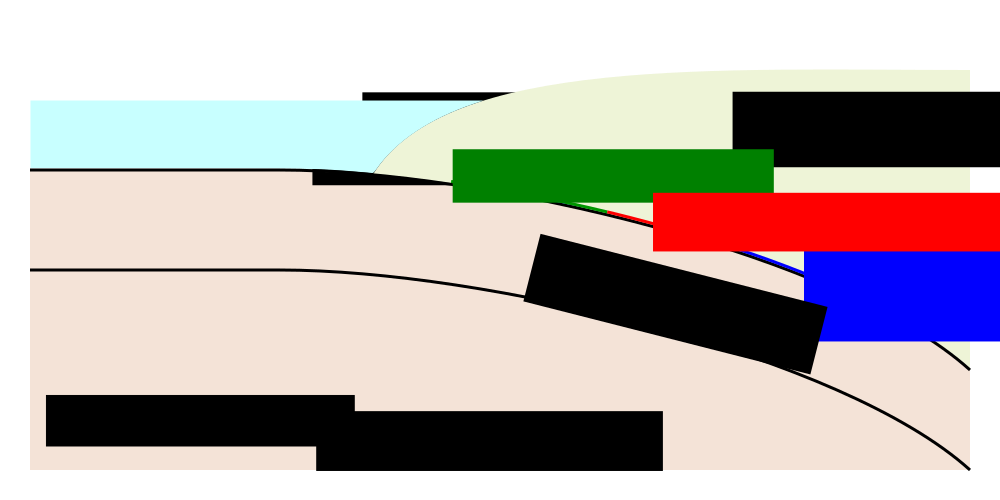
\includegraphics[trim={0cm 0cm 0cm 0cm}, clip, width=11cm]{subductionzone/subduction_0.eps}
		\end{center}
	\end{frame}

	%----------------------------------------------------------------------------------------------------------------------------------
	% Slow slip
	%----------------------------------------------------------------------------------------------------------------------------------

	\subsection{Sow slip}

	\begin{frame}
		\frametitle{Slow slip}
		\begin{center}
			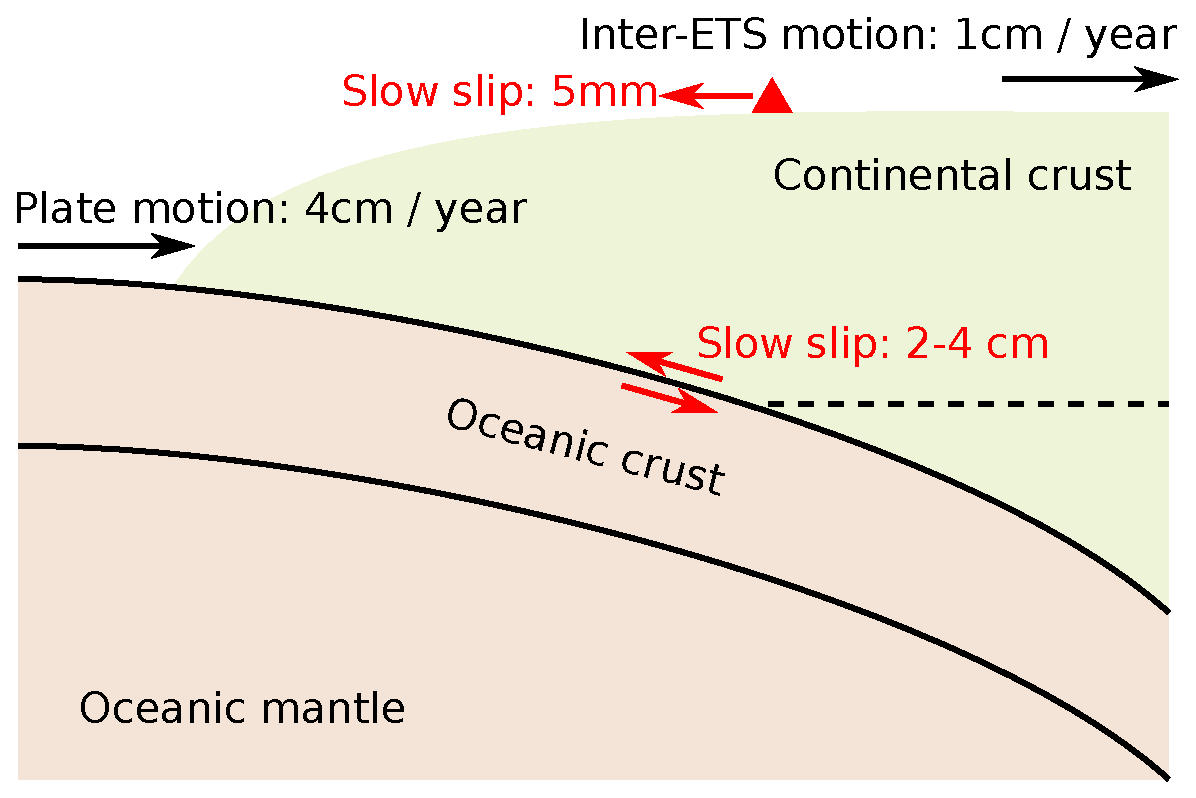
\includegraphics[trim={0cm 0cm 0cm 0cm}, clip, width=9cm]{ETS/slow_slip.eps}
		\end{center}
	\end{frame}

	\begin{frame}
		\frametitle{Slow slip}
		\begin{center}
			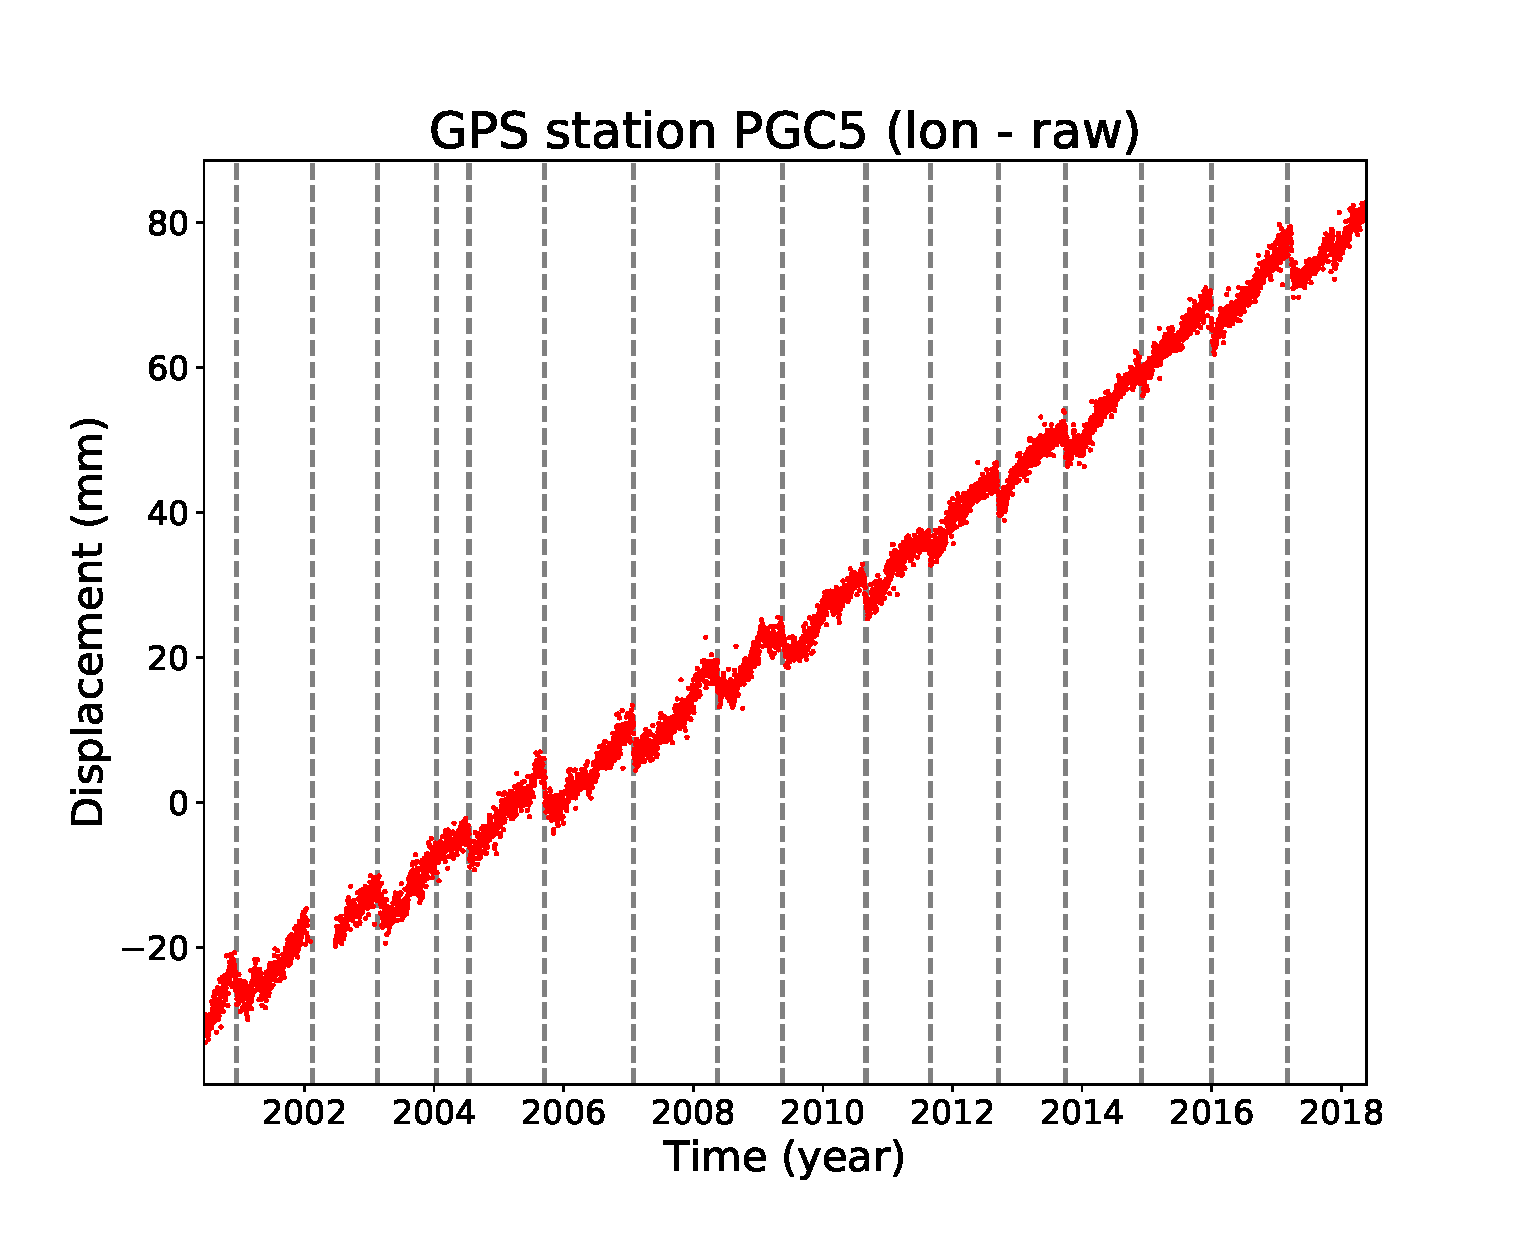
\includegraphics[trim={0cm 0cm 0cm 0cm}, clip, width=10cm]{slowslip/slow_slip_GPS.eps}
		\end{center}
	\end{frame}

	%----------------------------------------------------------------------------------------------------------------------------------
	% Tectonic tremor
	%----------------------------------------------------------------------------------------------------------------------------------

	\subsection{Tectonic tremor}

	\begin{frame}
		\frametitle{Tectonic tremor}
		\begin{itemize}
			\item Long (several seconds to many minutes)
			\item Low amplitude
			\item Emergent onsets
			\item Absence of clear impulsive phases
		\end{itemize}
	\end{frame}

	\begin{frame}
		\frametitle{Tectonic tremor}
		\begin{center}
			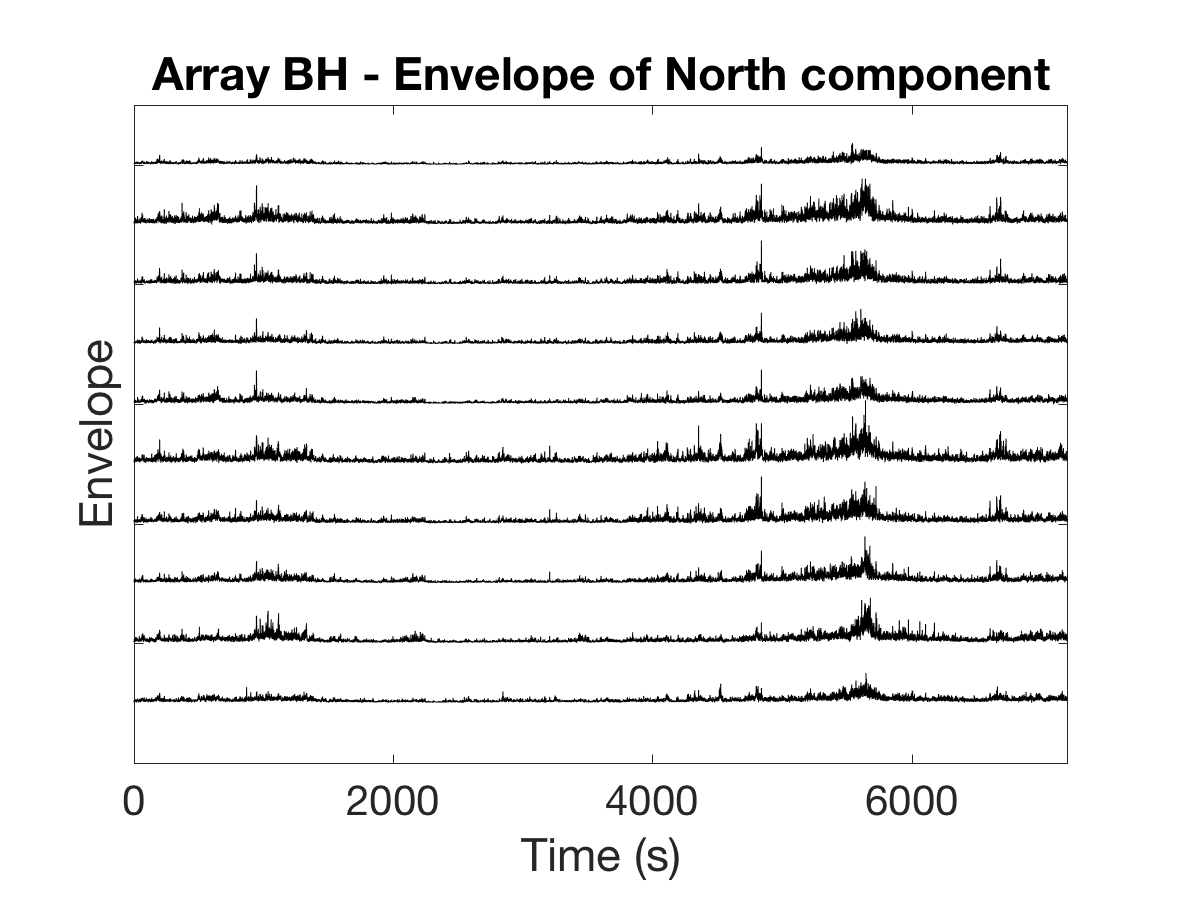
\includegraphics[trim={0cm 0cm 0cm 0cm}, clip, width=9cm]{ETS/tremor.eps}
		\end{center}
	\end{frame}

	%----------------------------------------------------------------------------------------------------------------------------------
	% Low-frequency earthquakes (LFE)
	%----------------------------------------------------------------------------------------------------------------------------------

	\subsection{Low-frequency earthquakes (LFE)}

	\begin{frame}
		\frametitle{Low-frequency earthquakes (LFE)}
		\begin{itemize}
			\item Small magnitude earthquakes (M $\sim$ 1)
			\item Frequency content (1-10 Hz) lower than for ordinary earthquakes (up to 20 Hz)
			\item Source located on the plate boundary,
			\item Focal mechanism: Shear slip on a low-angle thrust fault dipping in the same direction as the plate interface
		\end{itemize}
	\end{frame}

	\begin{frame}
		\frametitle{Low-frequency earthquakes (LFEs)}
		\begin{center}
			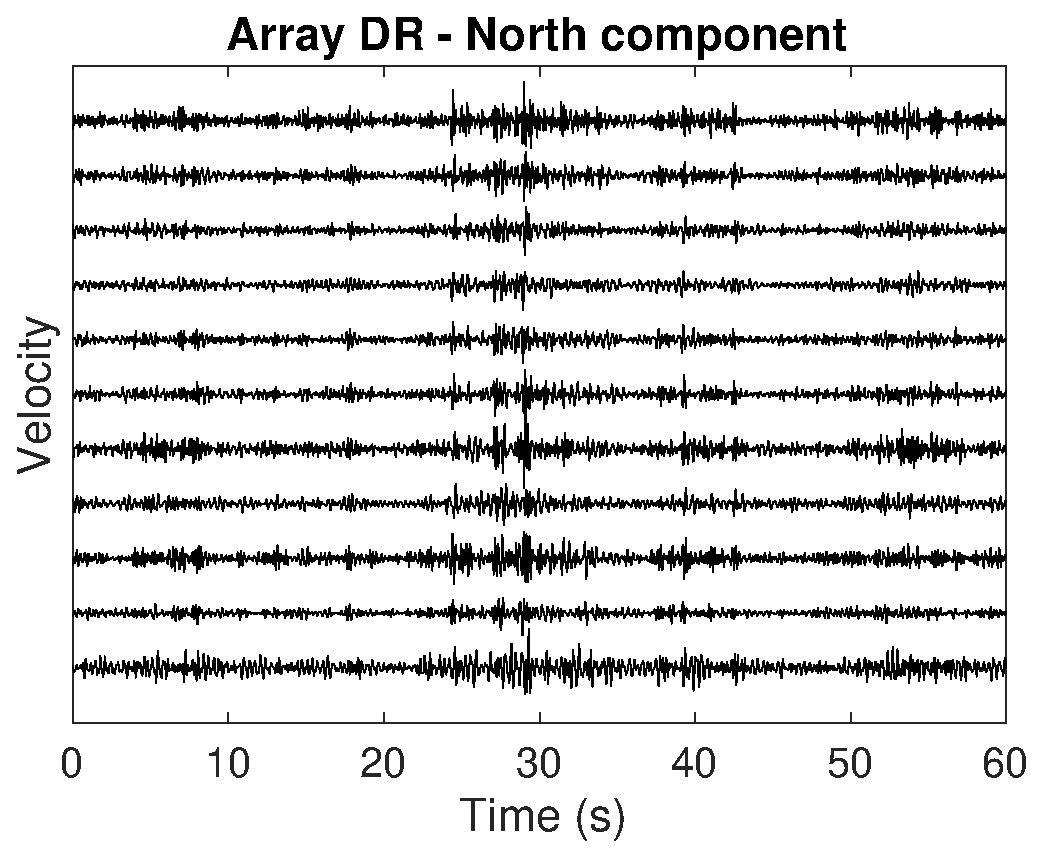
\includegraphics[trim={0cm 0cm 0cm 0cm}, clip, width=8cm]{ETS/LFE_NS.eps}
		\end{center}
	\end{frame}

	%----------------------------------------------------------------------------------------------------------------------------------
	% Episodic Tremor and Slip (ETS)
	%----------------------------------------------------------------------------------------------------------------------------------

	\subsection{Episodic Tremor and Slip (ETS)}

	\begin{frame}
		\frametitle{Episodic Tremor and Slip (ETS)}
		\begin{itemize}
			\item Tectonic tremor observations spatially and temporally correlated with slow slip observations (Nankai, Cascadia)
			\item Only biggest tremor episode associated with slow slip
			\item No spatial or temporal correlation in other regions like New Zealand
		\end{itemize}
	\end{frame}

	%----------------------------------------------------------------------------------------------------------------------------------
	% Research questions
	%----------------------------------------------------------------------------------------------------------------------------------
	
	\subsection{Research questions}

	\begin{frame}
		\frametitle{Depth of the source of the tectonic tremor in the eastern Olympic Peninsula}
		\begin{itemize}
			\item Lack of impulsive phases $\rightarrow$ Difficult to determine the depth of the source of the tremor
			\item Tectonic tremor is at least partly made of a swarm of LFEs
			\item LFEs are located on the plate boundary
		\end{itemize}

		\begin{block}{}
			$\rightarrow$ Research question: Is the source of the tectonic tremor located on the plate boundary? What is the depth extent of the location of the source of the tremor?
		\end{block}
	\end{frame}

	\begin{frame}
		\frametitle{A low-frequency earthquake catalog for southern Cascadia}
		\begin{itemize}
			\item LFE grouped into families of events
			\item All the earthquakes of a given family originate from the same small patch on the plate interface
			\item LFE recur more or less episodically in a bursty manner
			\item Wide range of recurrence behavior between seismic regions, and within the same seismic region
		\end{itemize}
	\end{frame}

	\begin{frame}
		\frametitle{LFE in Washington State}
		\begin{center}
			\includegraphics[trim={1cm 3cm 1cm 14cm}, clip, width=9cm]{LFE_catalogs/cascadia.eps}
		\end{center}
	\end{frame}

	\begin{frame}
		\frametitle{LFE on the San Andreas Fault}
		\begin{center}
			\includegraphics[trim={1cm 3cm 1cm 14cm}, clip, width=9cm]{LFE_catalogs/sanandreas.eps}
		\end{center}
	\end{frame}

	\begin{frame}
		\frametitle{A low-frequency earthquakes catalog for southern Cascadia}
		\begin{itemize}
			\item LFE families in southern Cascadia:
			\begin{itemize}
				\item 34 LFE families on the subduction zone
				\item 3 LFE families on two strike-slip faults from the San Andreas Fault system
			\end{itemize}
			\item Wide range of recurrence behavior between Washington State and the San Andreas Fault, and within the San Andreas Fault zone
		\end{itemize}
		
		\begin{block}{}
			$\rightarrow$ Do low-frequency earthquakes families behave similarly or differently in southern Cascadia, compared to Washington State and the San Andreas Fault?
		\end{block}
	\end{frame}

	\begin{frame}
		\frametitle{Detection of slow slip events in New Zealand}
		\begin{itemize}
			\item Small (M $\sim$ 5) or long (several months) slow slip events are harder to detect
			\item In Cascadia, Mexico, tremor used as a proxy to study slow slip events
			\item Different pattern in northern new Zealand:
			\begin{itemize}
				\item Tremor source located downdip of the slow slip on the plate boundary
				\item Tremor activity does not seem to increase during slow slip events
			\end{itemize}
		\end{itemize}

		\begin{block}{}
			$\rightarrow$ Can we detect smaller and / or longer slow slip events in the absence of spatially and temporally correlated tectonic tremor?
		\end{block}			
	\end{frame}

	%----------------------------------------------------------------------------------------------------------------------------------
	% Depth of the source of the tectonic tremor
	%----------------------------------------------------------------------------------------------------------------------------------
				
	\section{Depth of the source of the tectonic tremor}

	\begin{frame}
		\frametitle{Depth of the source of the tectonic tremor}
		\tableofcontents[currentsection,hideothersubsections]
	\end{frame}

	\subsection{Motivation}

	\begin{frame}
		\frametitle{Tremor and LFEs}
		\begin{itemize}
			\item Tremor can be explained as a swarm of LFEs
			\item LFE occur as shear faulting on the subduction-zone plate interface
		\end{itemize}

		Shelly et al. (2007), Ide et al. (2007)
	\end{frame}

	\begin{frame}
		\frametitle{High pore fluid pressure in the oceanic crust}
		\begin{center}
			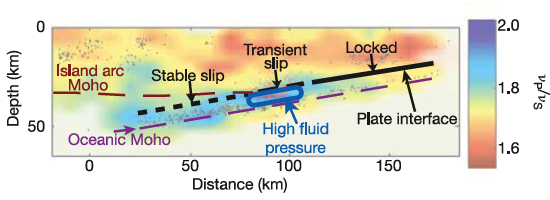
\includegraphics[trim={0cm 0cm 0cm 0cm}, clip, width=11cm]{articles/shelly_al_2006_4d.png}
		\end{center}
	\end{frame}

	\begin{frame}
		\frametitle{High pore fluid pressure in the oceanic crust}
		\begin{center}
			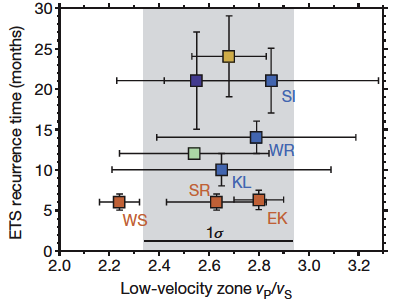
\includegraphics[trim={0cm 0cm 0cm 0cm}, clip, width=9cm]{articles/audet_burgmann_2014_1b.png}
		\end{center}
	\end{frame}

	\begin{frame}
		\frametitle{Fracture network}
		\begin{center}
			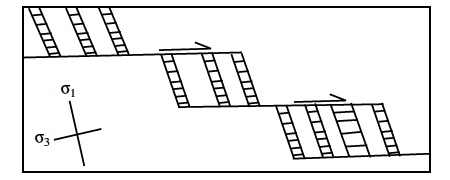
\includegraphics[trim={0cm 0cm 0cm 0cm}, clip, width=10cm]{articles/fagereng_harris_2014_8b.png}
		\end{center}
	\end{frame}

	\begin{frame}
		\frametitle{Low $V_P / V_S$ ratio in subduction zones}
		\begin{center}
			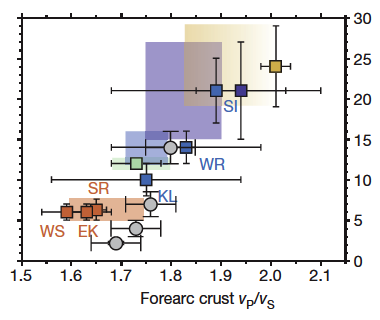
\includegraphics[trim={0cm 0cm 0cm 0cm}, clip, width=9cm]{articles/audet_burgmann_2014_1c.png}
		\end{center}
	\end{frame}

	\begin{frame}
		\frametitle{Low $V_P / V_S$ ratio in the overriding plate}
		\begin{center}
			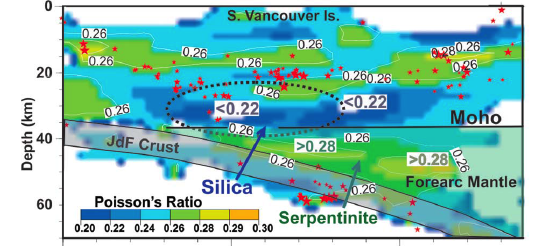
\includegraphics[trim={0cm 0cm 0cm 0cm}, clip, width=11cm]{articles/hyndmann_al_2015_8a.png}
		\end{center}
	\end{frame}

	\begin{frame}
		\frametitle{Inferred location of the source of the tremor}
		\begin{center}
			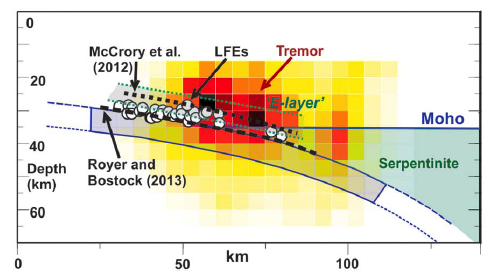
\includegraphics[trim={0cm 0cm 0cm 0cm}, clip, width=11cm]{articles/hyndmann_al_2015_8b.png}
		\end{center}
	\end{frame}

	\begin{frame}
		\frametitle{Where is the source of the tremor located?}
		\begin{itemize}
			\item Same location as LFEs $\rightarrow$ Very thin layer at the plate boundary
			\item Same location as quartz $\rightarrow$ Thick layer above the plate boundary, in the continental crust
		\end{itemize}

		\begin{block}{}
			$\rightarrow$ How to constrain better the location of the source of the tremor?
		\end{block}
	\end{frame}

	\subsection{Data}

	\begin{frame}
		\frametitle{Cascadia Array of Arrays}
		\begin{columns}[c]
			\begin{column}{5cm}
				\begin{itemize}
					\item Cascadia Array of Arrays experiment (2009-2010)

					%\vspace{1em}

					\item Eight arrays of seismic stations in the Olympic Peninsula

					%\vspace{1em}

					\item Recorded the main ETS event in August 2010, and the 2011 ETS event

					%\vspace{1em}

					\item Tremor located just under the arrays
				\end{itemize}
			\end{column}
			\begin{column}{7cm}
				\begin{center}
					\includegraphics[trim={0cm 1cm 0cm 9.5cm}, clip, width=7cm]{AoA/arrays_location.eps}
				\end{center}
			\end{column}
		\end{columns}
	\end{frame}

	\begin{frame}
		\frametitle{Tremor catalog}
		\begin{itemize}
			\vspace{1em}

			\item 28902 one-minute-long time windows where tectonic tremor is recorded

			\vspace{1em}

			\item For each tremor window: Beginning time, latitude, longitude, and depth of the tremor source

			\vspace{1em}

			\item Start date: June 20\textsuperscript{th} 2009

			\vspace{1em}

			\item End date: September 30\textsuperscript{th} 2010
		\end{itemize}
		\btVFill
		\tiny{Ghosh A., Vidale J.E., Creager K.C. (2012). \textit{JGR}, \textbf{117}, B10301.}
	\end{frame}

	\subsection{Method}

	\begin{frame}
		\frametitle{Stacking of tremor recordings}
		\begin{itemize}
			\item Tectonic tremor recorded at the Big Skidder array and which source is located in a 5x5 km cell just under the array
			\item 70 one-minute-second-long time windows
			\item For each time window:
			\begin{itemize}
				\item For each station, cross-correlate the horizontal component with the vertical component
				\item Stack (linearly) the cross-correlation over all the stations of the array
			\end{itemize}
			\item Plot all the 70 stacked cross-correlation
			\item Stack the 70 signals with a linear, power, or phase-weighted stack
		\end{itemize}
	\end{frame}

	\begin{frame}
		\frametitle{Stacking of tremor recordings}
		\begin{center}
			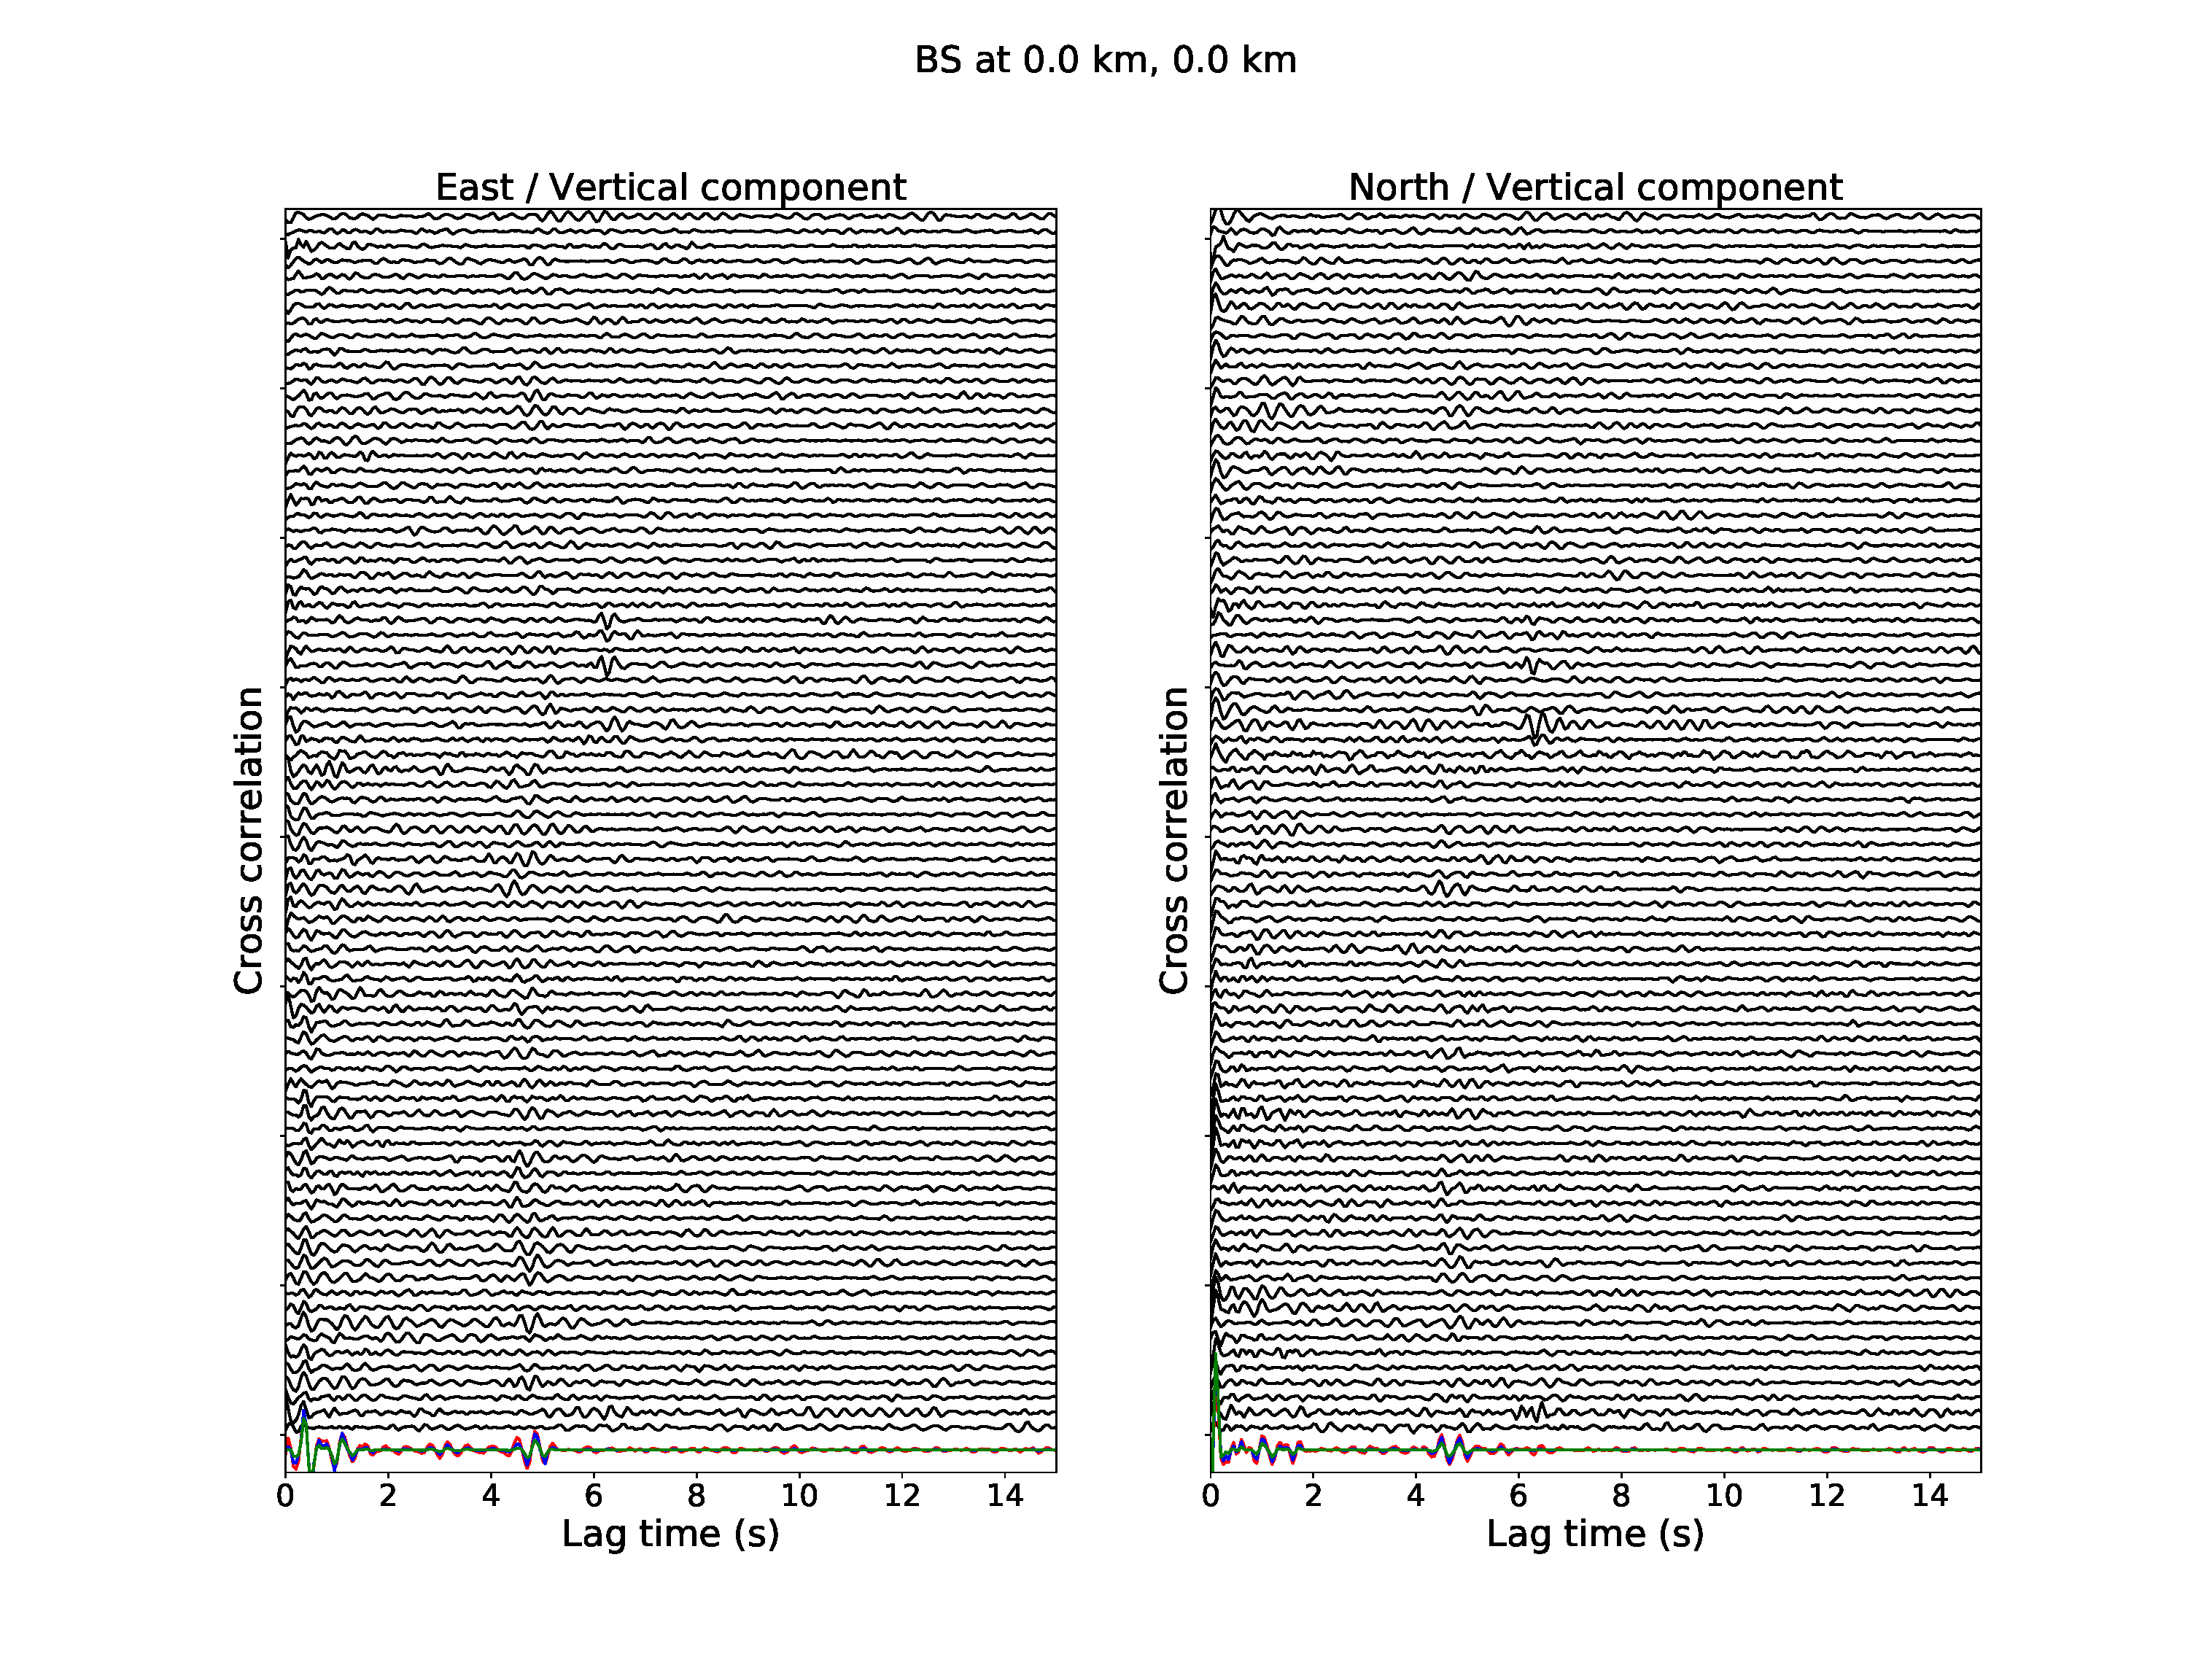
\includegraphics[width=8cm, trim={5cm 2cm 5cm 3.5cm}, clip]{BS_000_000/BS_000_000_lin.eps}
		\end{center}
	\end{frame}
		
	\begin{frame}
		\frametitle{Clustering of cross correlation functions} 
		Does the cross-correlation for a given one-minute-long time windows look like the stack over all time windows?

		\begin{itemize}
			\item Ratio RMS between 4 and 6 s / RMS between 12 and 14 s
			\item Cross-correlation between one cross-correlation and the stack:
			\begin{itemize}
				\item Maximum cross-correlation value
				\item Cross-correlation at time lag 0
				\item Time lag corresponding to the maximum cross-correlation value
			\end{itemize}
		\end{itemize}

		$\rightarrow$ K-means clustering $\rightarrow$ Two clusters (good time windows / bad time windows)
	\end{frame}

	\begin{frame}
		\frametitle{Clustering of cross correlation functions}
		\begin{center}
			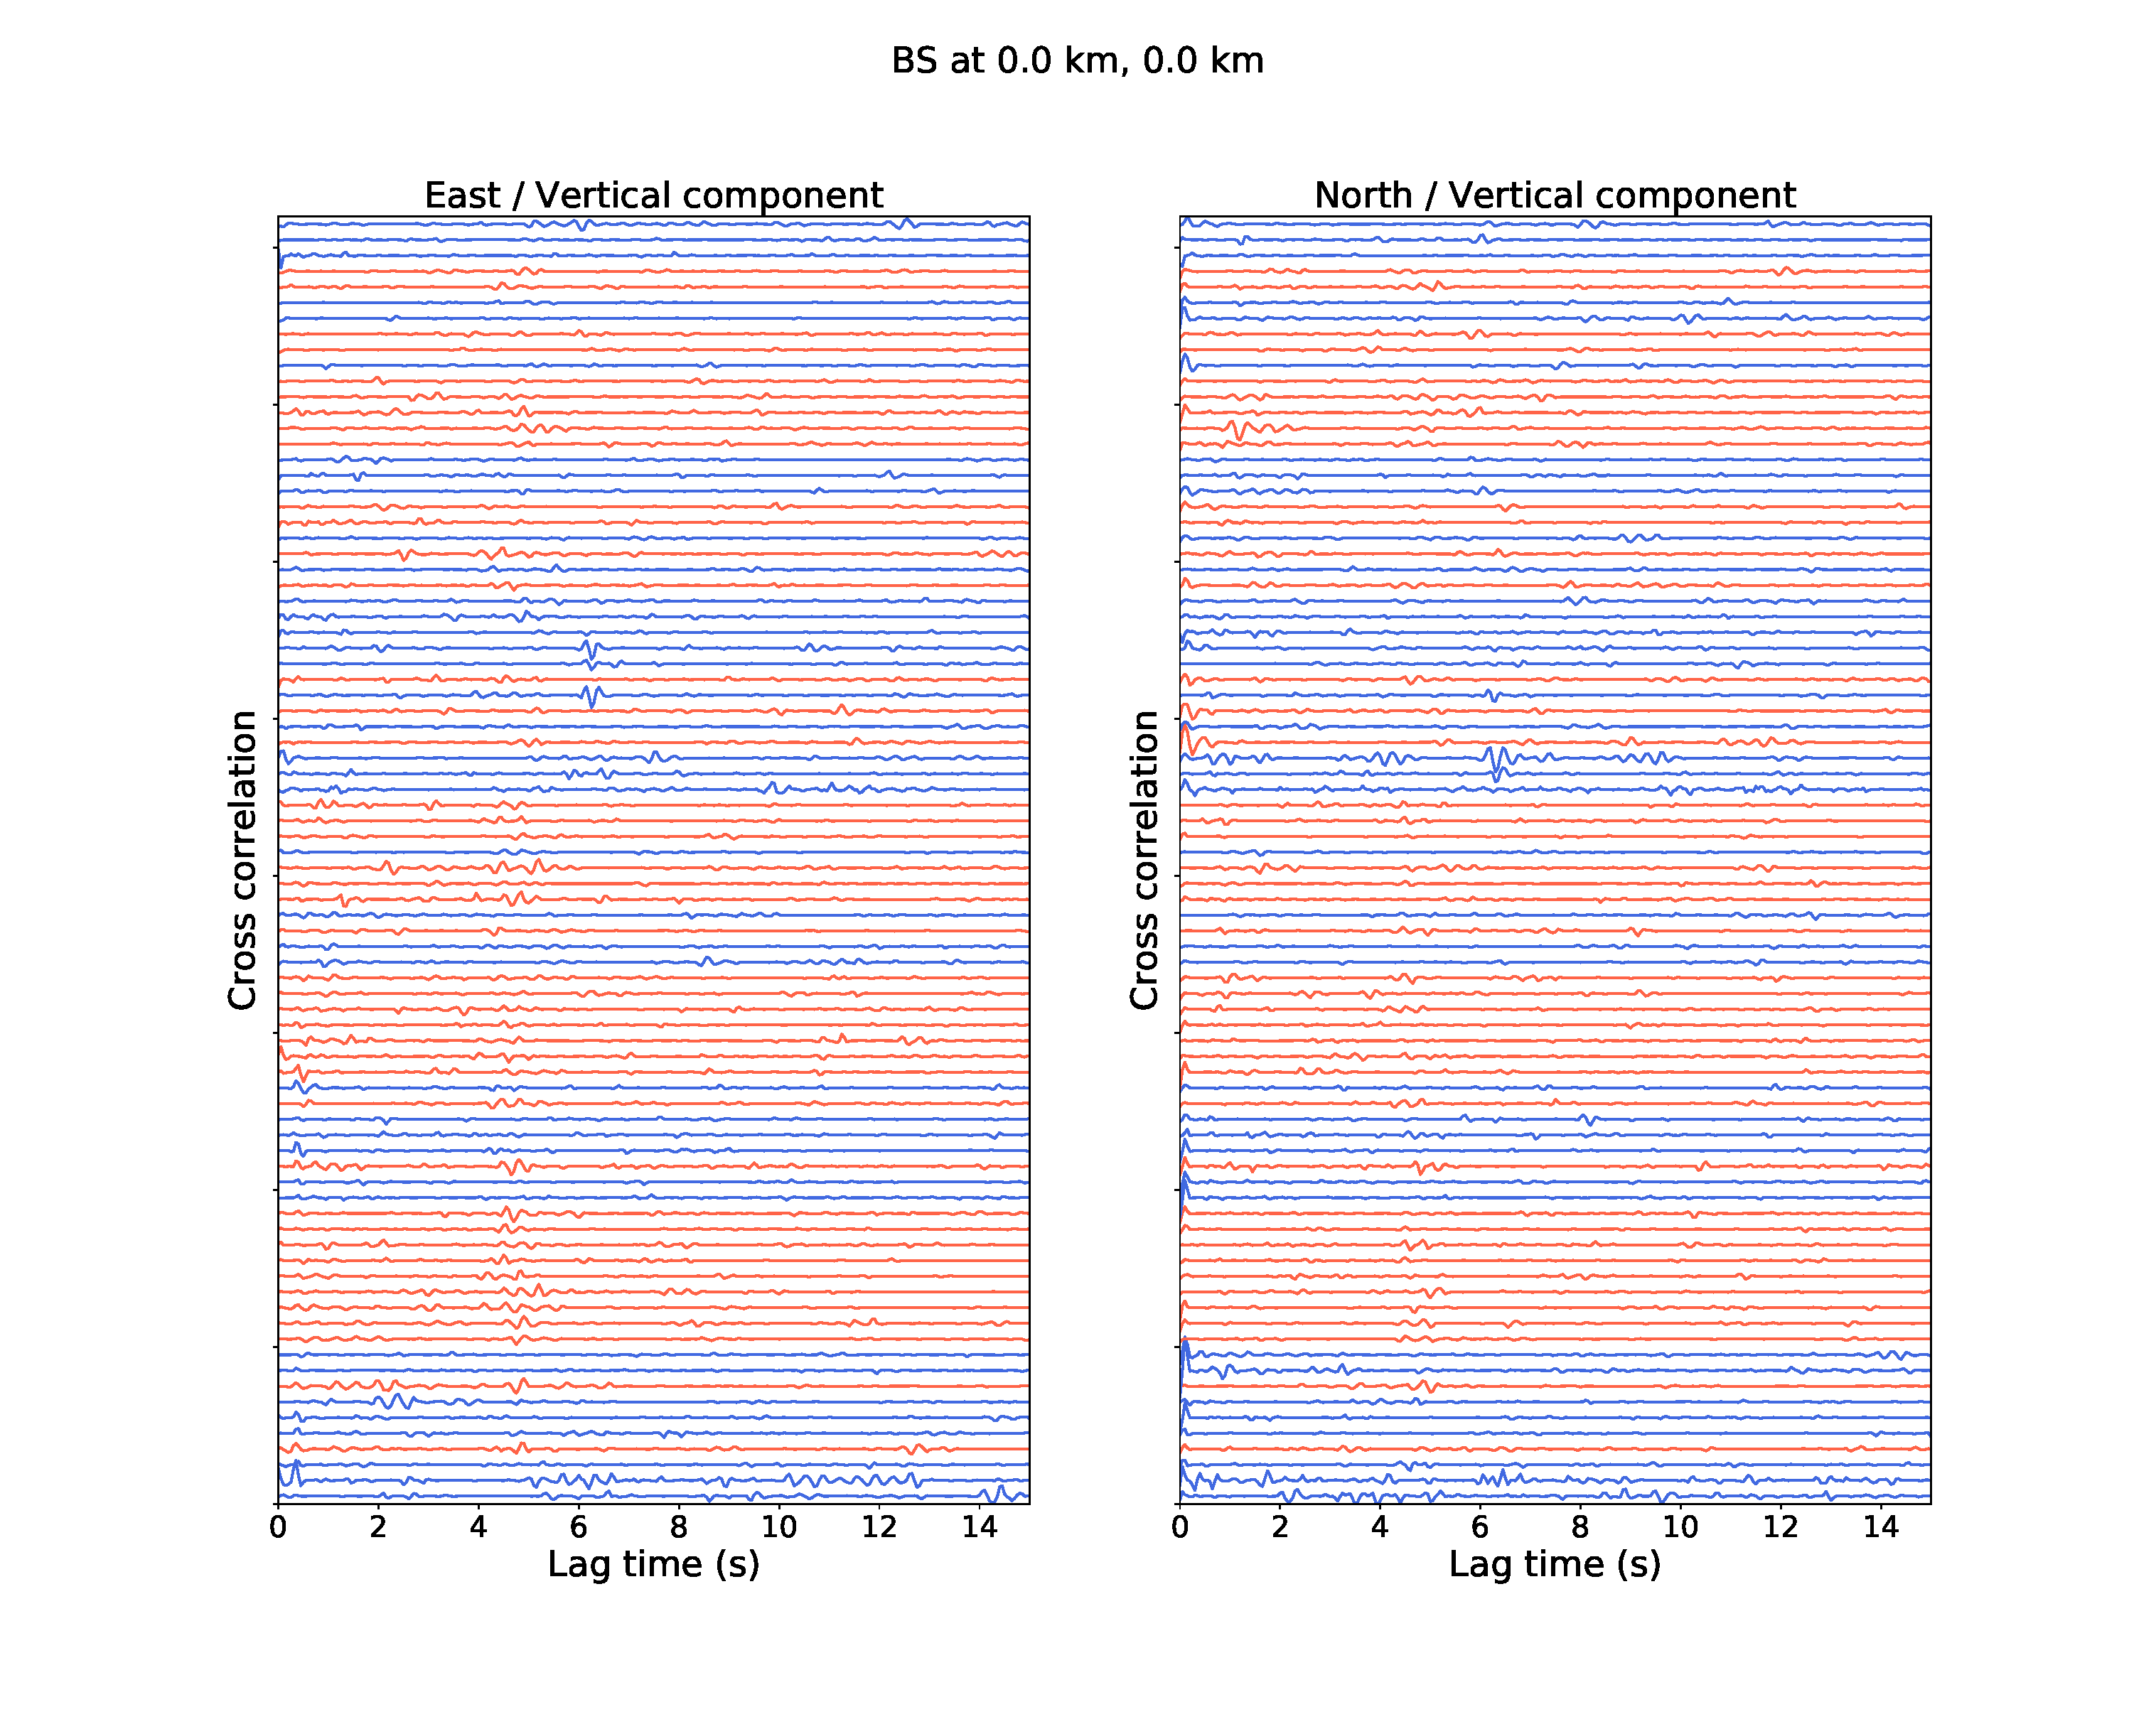
\includegraphics[width=7.5cm, trim={5cm 2.5cm 5cm 4cm}, clip]{BS_000_000/BS_000_000_PWS_PWS_cluster_ccwin.eps}
		\end{center}
	\end{frame}

	\begin{frame}
		\frametitle{Stacked cross correlation}
		\begin{center}
			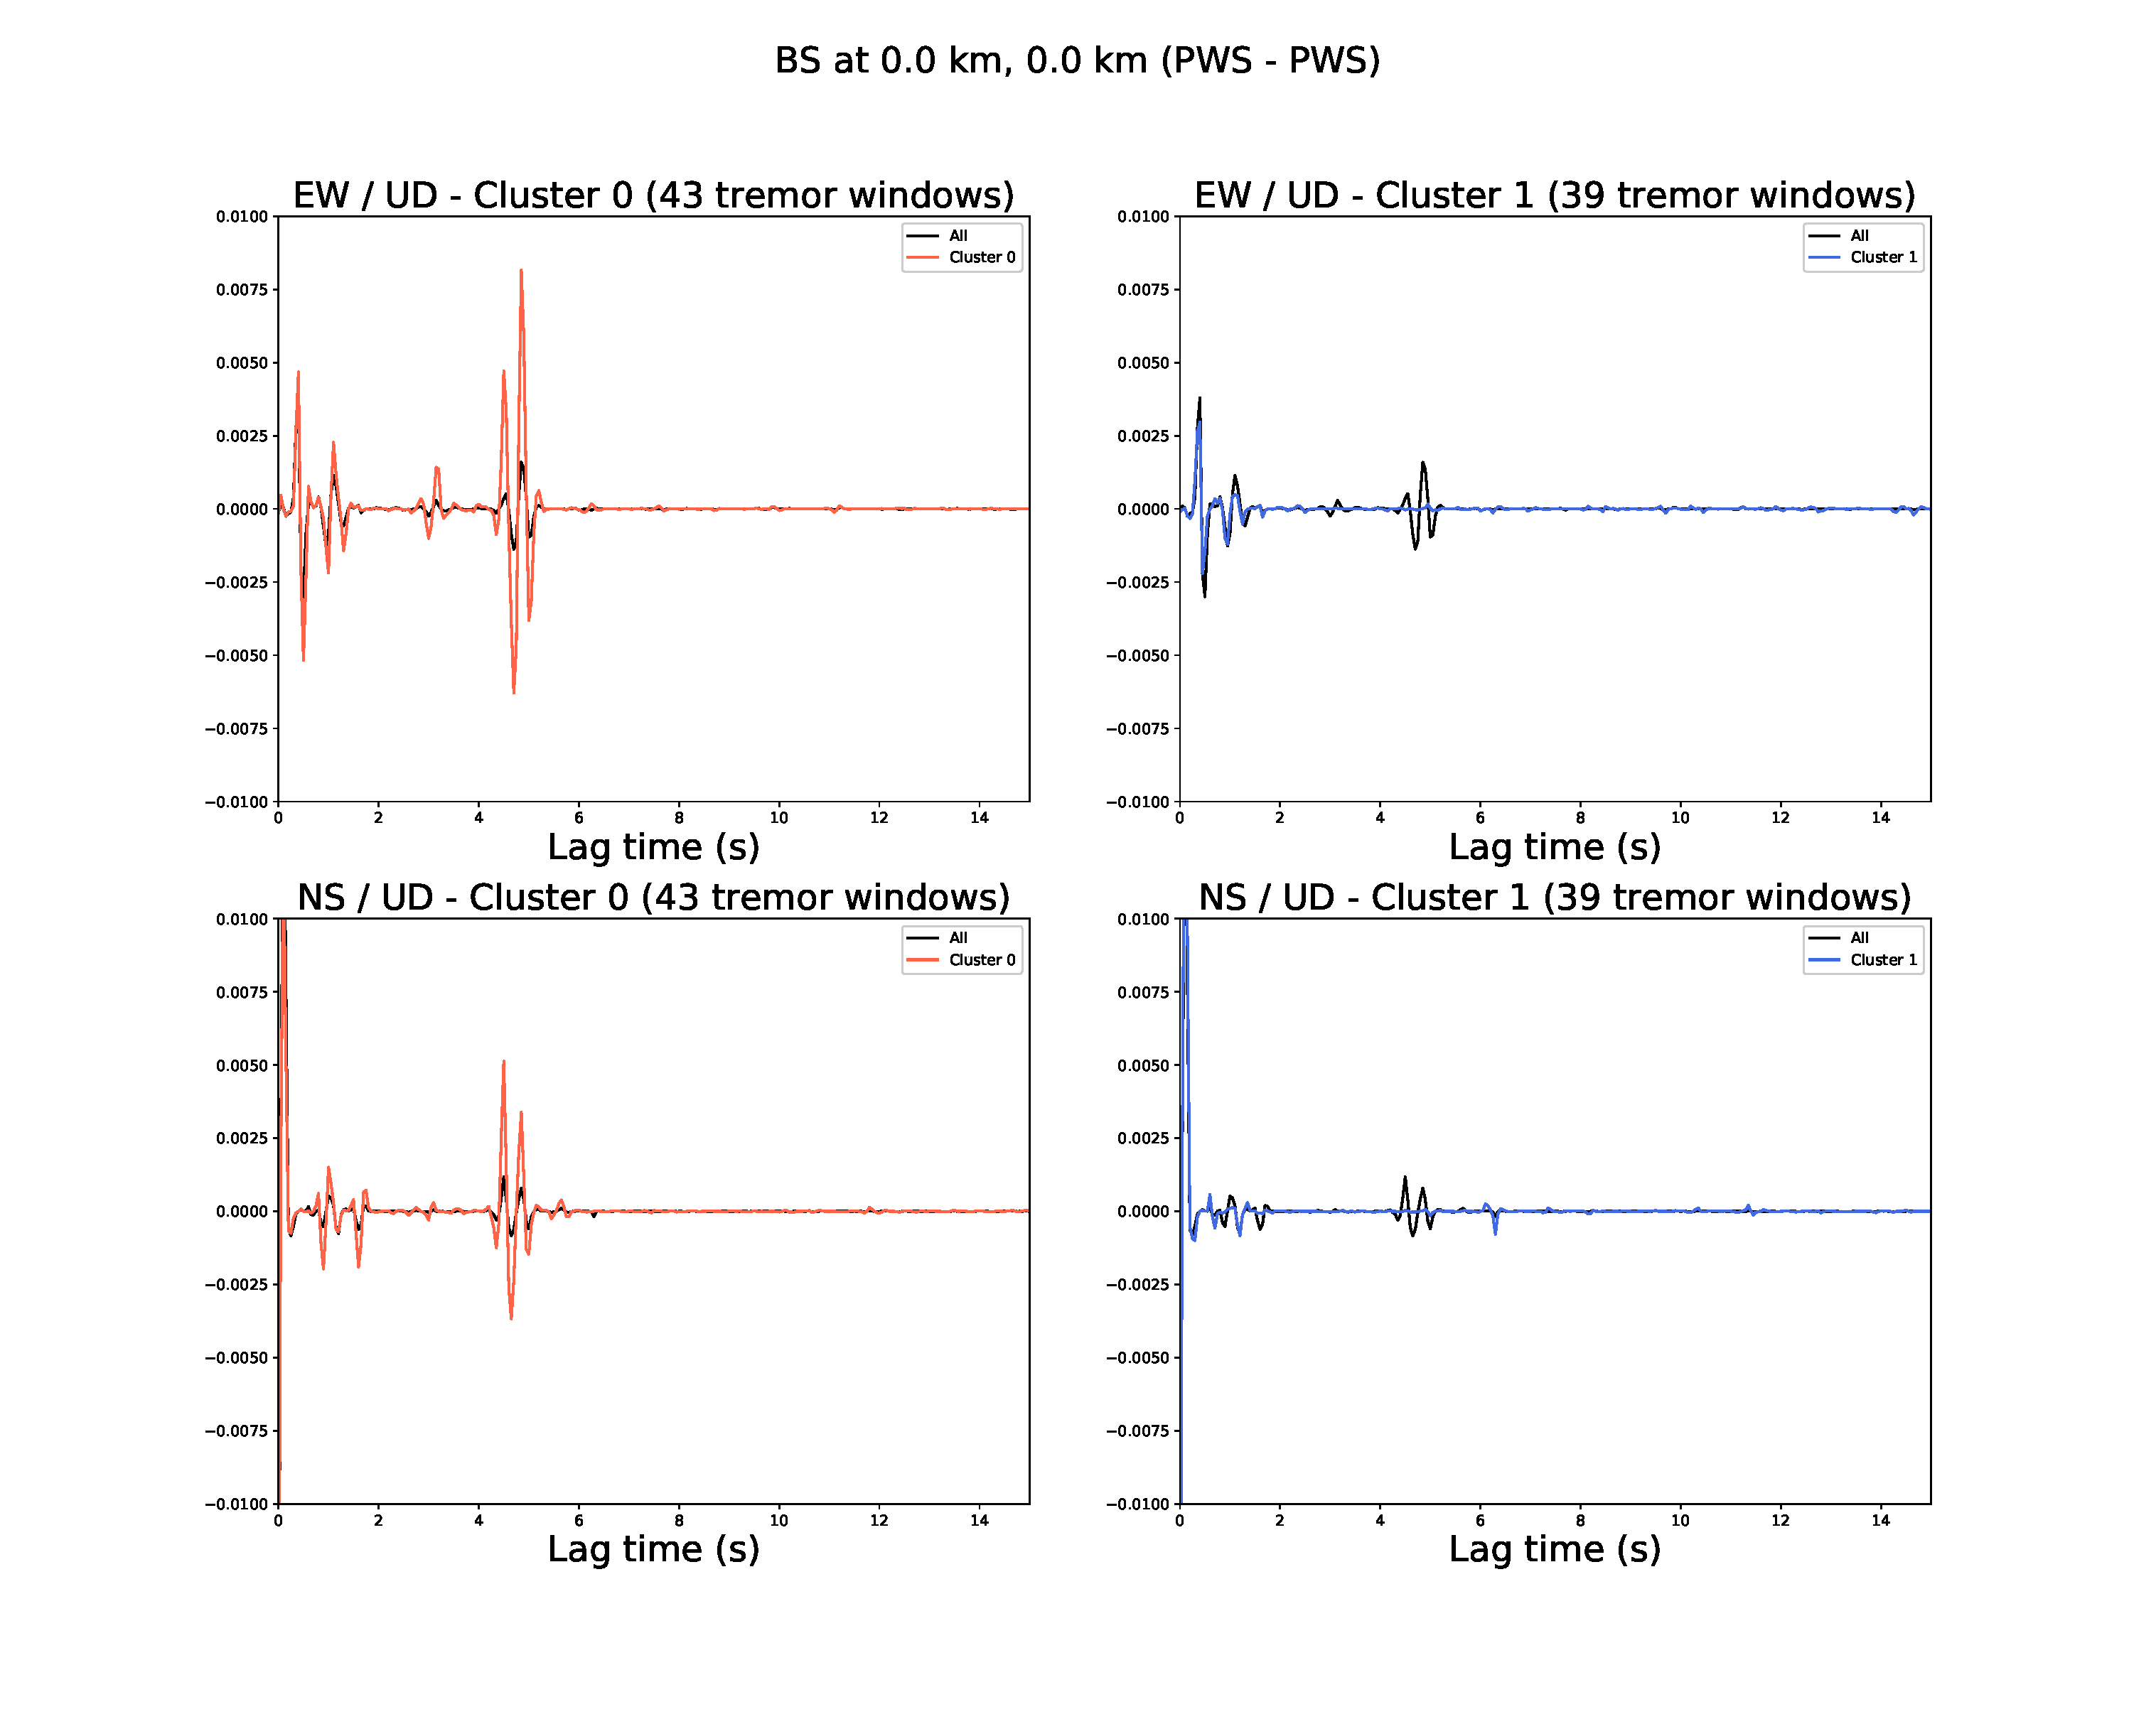
\includegraphics[width=8cm, trim={4.5cm 2.5cm 5cm 4cm}, clip]{BS_000_000/BS_000_000_PWS_PWS_cluster_stackcc.eps}
		\end{center}
	\end{frame}

	\subsection{Results}

	\begin{frame}
		\frametitle{Distance to plate boundary}
		\begin{center}
			\includegraphics[width=6cm, trim={1cm 3cm 2cm 6cm}, clip]{other/d_to_pb_PWS_PWS.eps}
		\end{center}
	\end{frame}

	\begin{frame}
		\frametitle{Interpolation}
		\begin{itemize}
			\item Number of tremor
			\item ratio peak cc / RMS
			\item Distance to array (strike / dip)
		\end{itemize}

		$\rightarrow$ Weights for interpolation of results from 8 arrays
	\end{frame}

	\begin{frame}
		\frametitle{Distance to plate boundary}
		% here map with all the arrays
	\end{frame}

	\subsection{Discussion and Conclusion}

	\begin{frame}
		\frametitle{Distribution of time lags}
		% Here histograms
	\end{frame}

	\begin{frame}
		\frametitle{Width of the distribution}
	\end{frame}

	\begin{frame}
		\frametitle{Thickness of the tremor zone}
		\begin{center}
			\includegraphics[width=6cm, trim={1cm 3cm 2cm 6cm}, clip]{other/thickness_PWS_PWS.eps}
		\end{center}
	\end{frame}

	\begin{frame}
		\frametitle{Conclusion}
		% ???
	\end{frame}

	%----------------------------------------------------------------------------------------------------------------------------------
	% A low-frequency earthquakes catalog for southern Cascadia
	%----------------------------------------------------------------------------------------------------------------------------------

	\section{A low-frequency earthquakes catalog for southern Cascadia}

	\begin{frame}
		\frametitle{A low-frequency earthquakes catalog for southern Cascadia}
		\tableofcontents[currentsection,hideothersubsections]
	\end{frame}

	%----------------------------------------------------------------------------------------------------------------------------------
	% Extension of an LFE catalog for southern Cascadia
	%----------------------------------------------------------------------------------------------------------------------------------

	\subsection{Extension of an LFE catalog for southern Cascadia}
	
	\begin{frame}
		\frametitle{Current catalog}
		\begin{center}
			\includegraphics[trim={1cm 3cm 1cm 8cm}, clip, width=7cm]{catalog_SC/families_map.eps}
		\end{center}
	\end{frame}

	\begin{frame}
		\frametitle{Current catalog}
		\begin{itemize}
			\item Subduction zone families
			\begin{itemize}
				\item 34 families
				\item Period covered: April 2008
				\item One burst of LFE lasting a few days and propagating from south to north
			\end{itemize}
			\item Strike-slip fault families
			\begin{itemize}
				\item 3 families
				\item Period covered: March and April 2008
				\item Active all the time, several bursts of LFE
			\end{itemize}
		\end{itemize}
	\end{frame}

	\begin{frame}
		\frametitle{Creating templates}
		% here procedure
	\end{frame}

	\begin{frame}
		\frametitle{Templates for permanent station KRMB}
		\begin{center}
			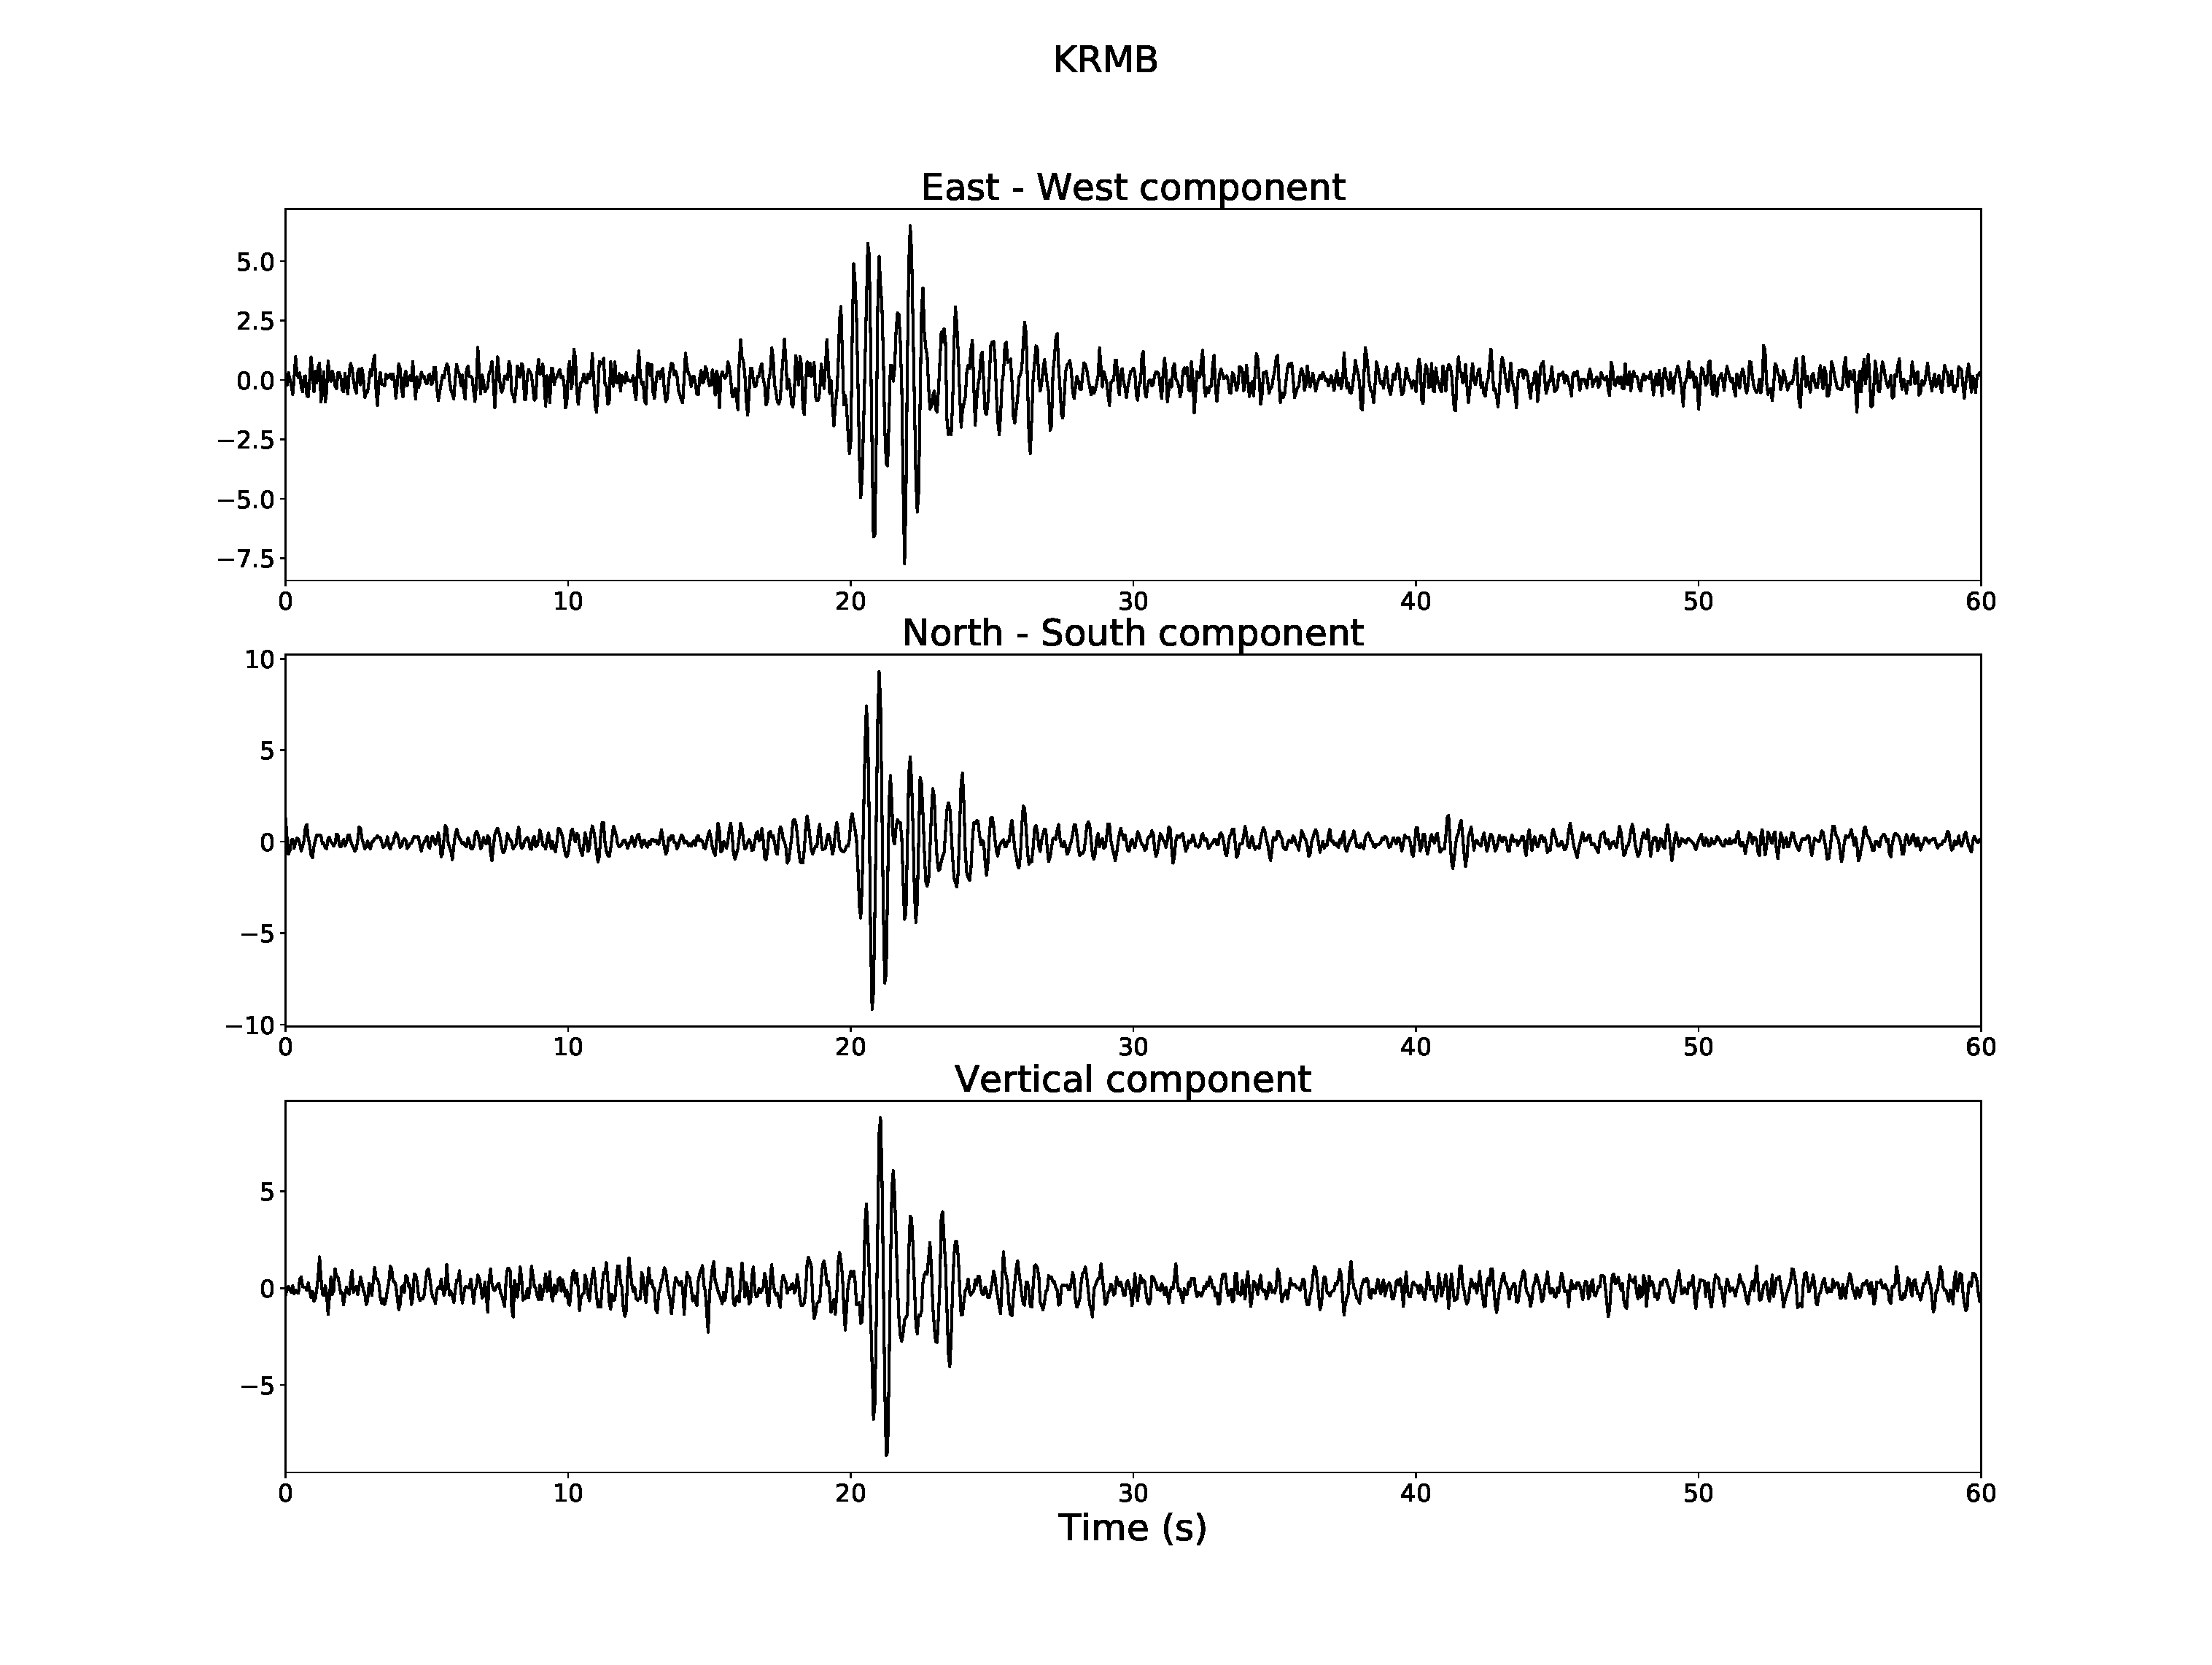
\includegraphics[width=8cm, trim={4cm 2cm 4cm 3cm}, clip]{catalog_SC/08042114048_KRMB.eps}
		\end{center}
	\end{frame}

	\begin{frame}
		\frametitle{Finding new LFE}
		% here metod
	\end{frame}

	\begin{frame}
		\frametitle{Analysis of one hour of seismic data}
		\begin{center}
			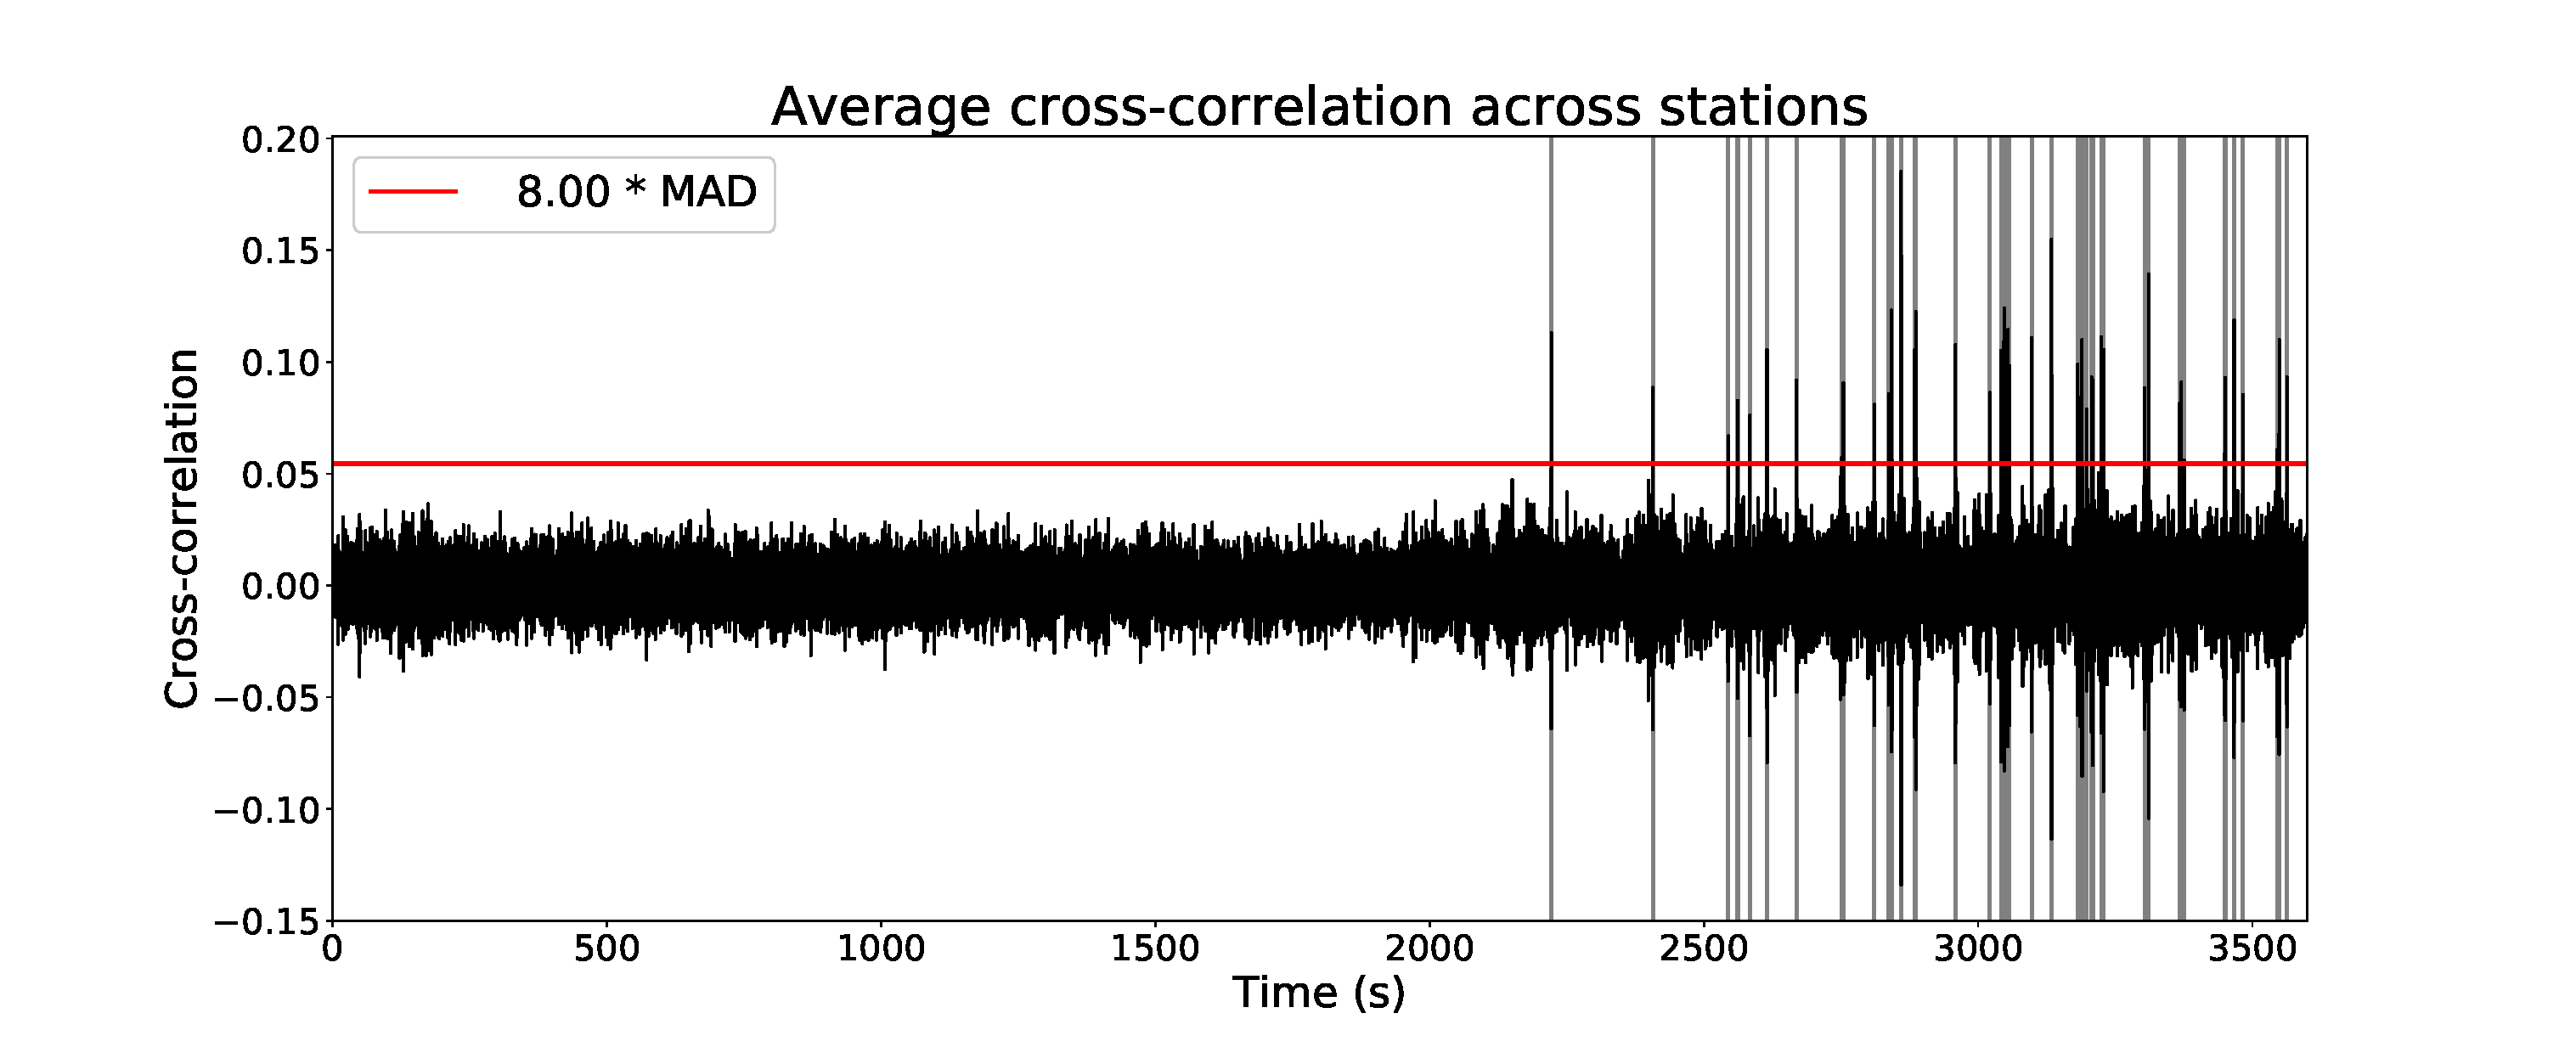
\includegraphics[width=11cm, trim={0cm 0cm 0cm 0cm}, clip]{catalog_SC/20080421_130000.eps}
		\end{center}
	\end{frame}

	\begin{frame}
		\frametitle{Comparison with existing catalog}
		\begin{center}
		Family 080421.14.048

		\vspace{2em}

		\begin{tabular}{| l | c |}
			\hline
			Number of LFE in my catalog & 236 \\
			\hline
			Number of LFE in the catalog by Plourde \textit{et al.} & 225 \\
			\hline
			Number of LFE added in my catalog & 13 \\
			\hline
			Number of LFE missing in my catalog & 2 \\
			\hline
			Number of LFE present in both catalogs & 223 \\
			\hline
		\end{tabular}
		\end{center}
	\end{frame}

	\begin{frame}
		\frametitle{Extension of the catalog}
		\begin{center}
			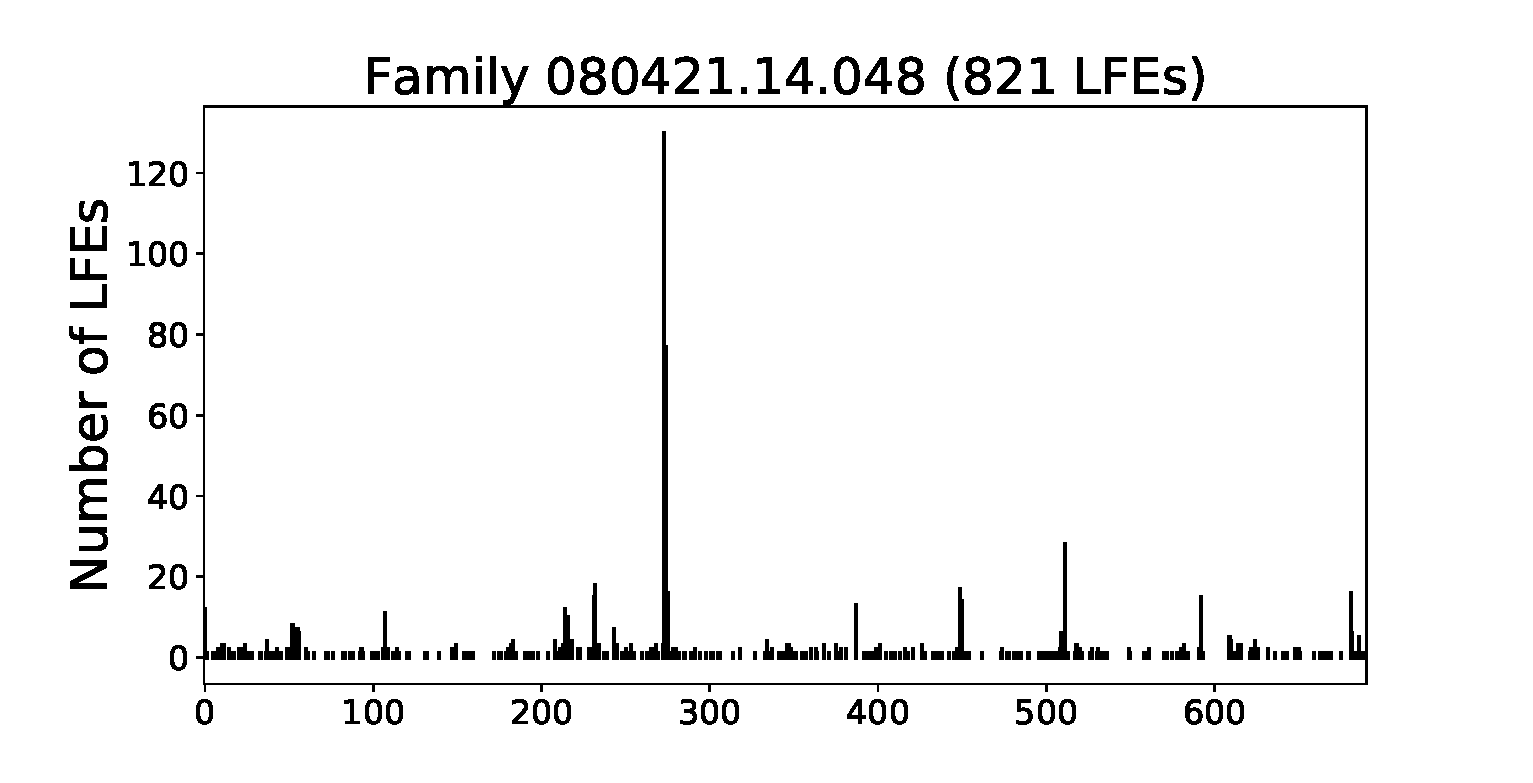
\includegraphics[width=11cm, trim={0cm 0cm 0cm 0cm}, clip]{catalog_SC/08042114048_FAME.eps}
		\end{center}
	\end{frame}
	
	\begin{frame}
		\frametitle{Extension of the catalog}
		\begin{center}
			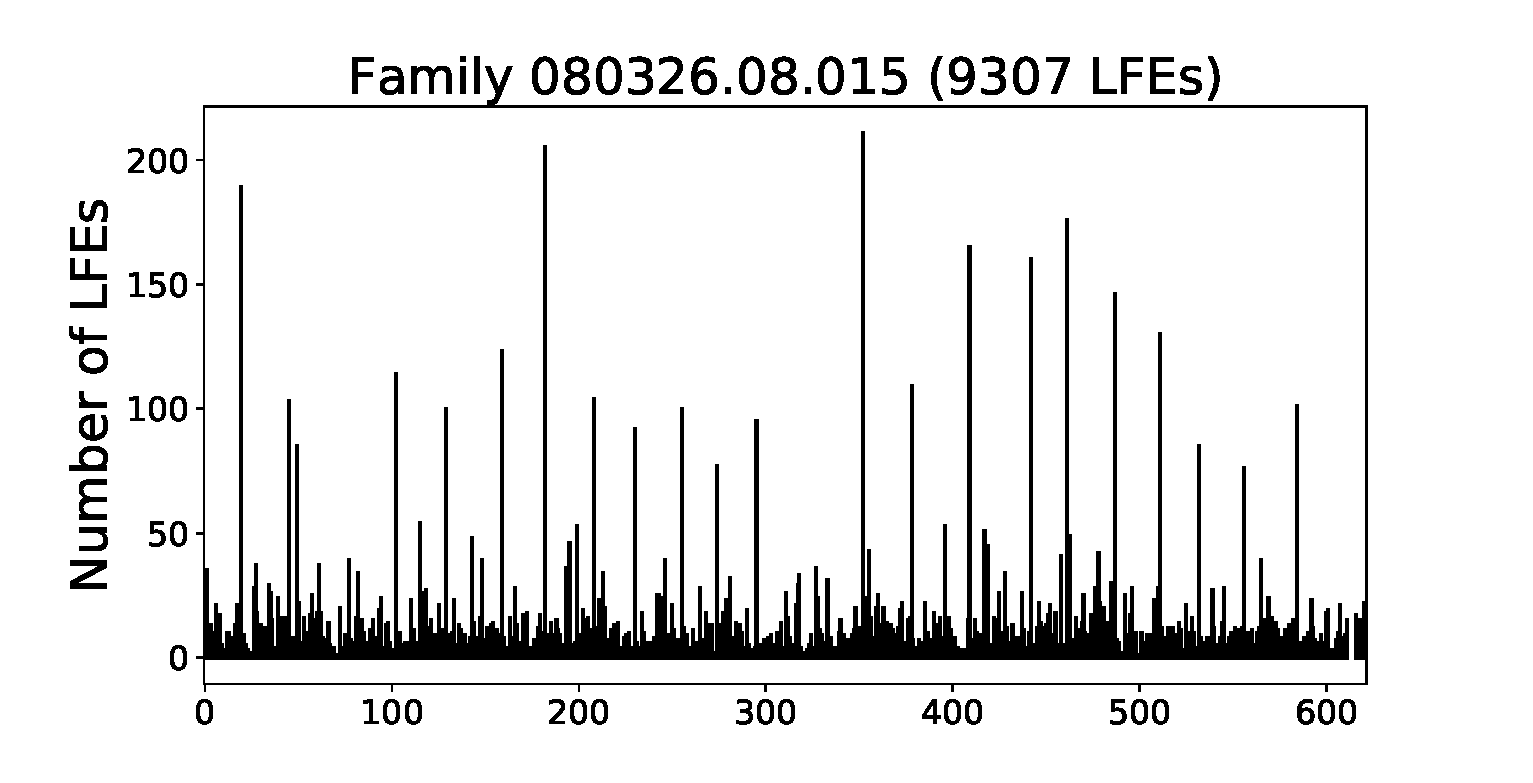
\includegraphics[width=11cm, trim={0cm 0cm 0cm 0cm}, clip]{catalog_SC/08032608015_FAME.eps}
		\end{center}
	\end{frame}

	\begin{frame}
		\frametitle{Detection of LFE with permanent networks}
		\begin{center}
			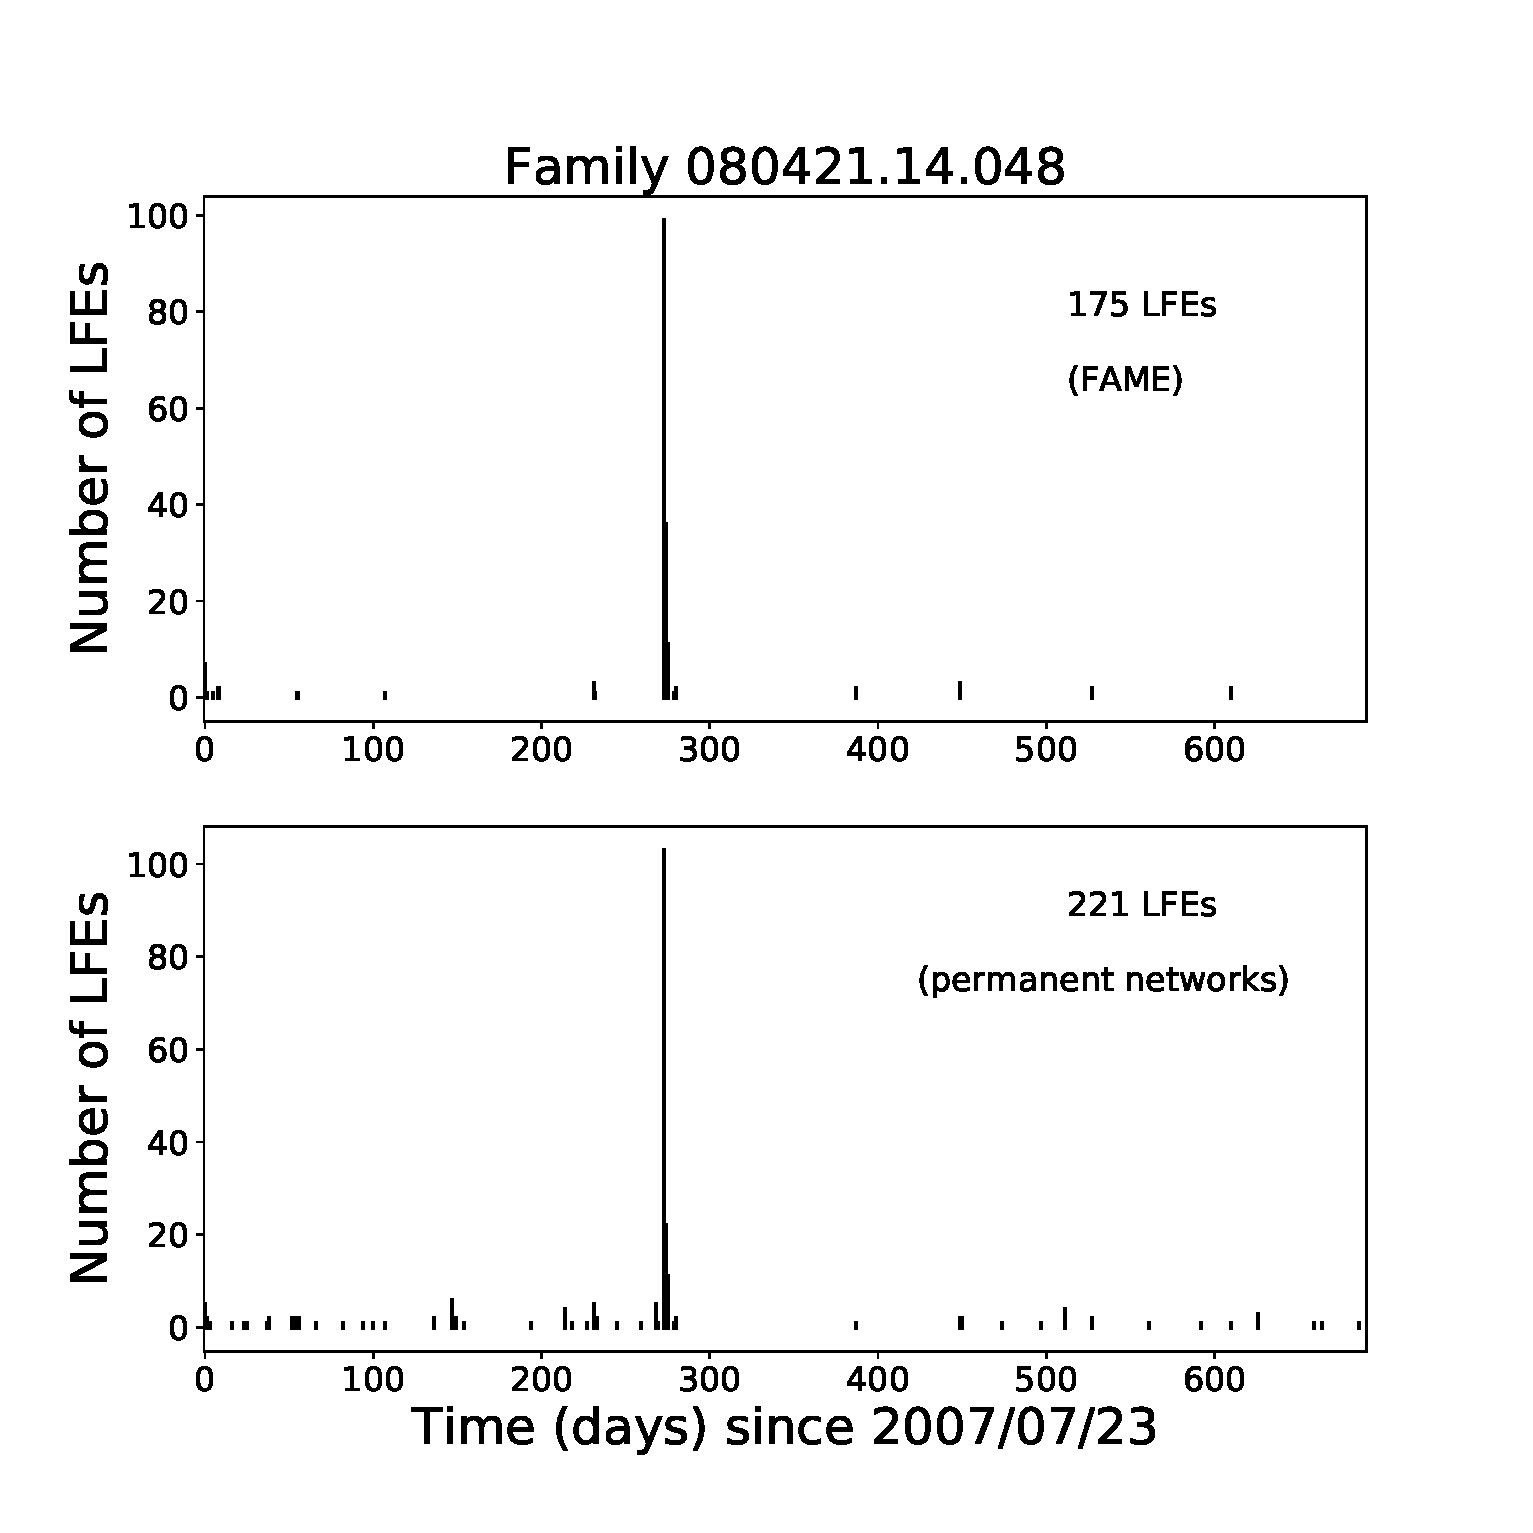
\includegraphics[width=7cm, trim={0cm 0cm 0cm 2cm}, clip]{catalog_SC/08042114048_permanent.eps}
		\end{center}
	\end{frame}

	\begin{frame}
		\frametitle{Detection of LFE with permanent networks}
		\begin{center}
			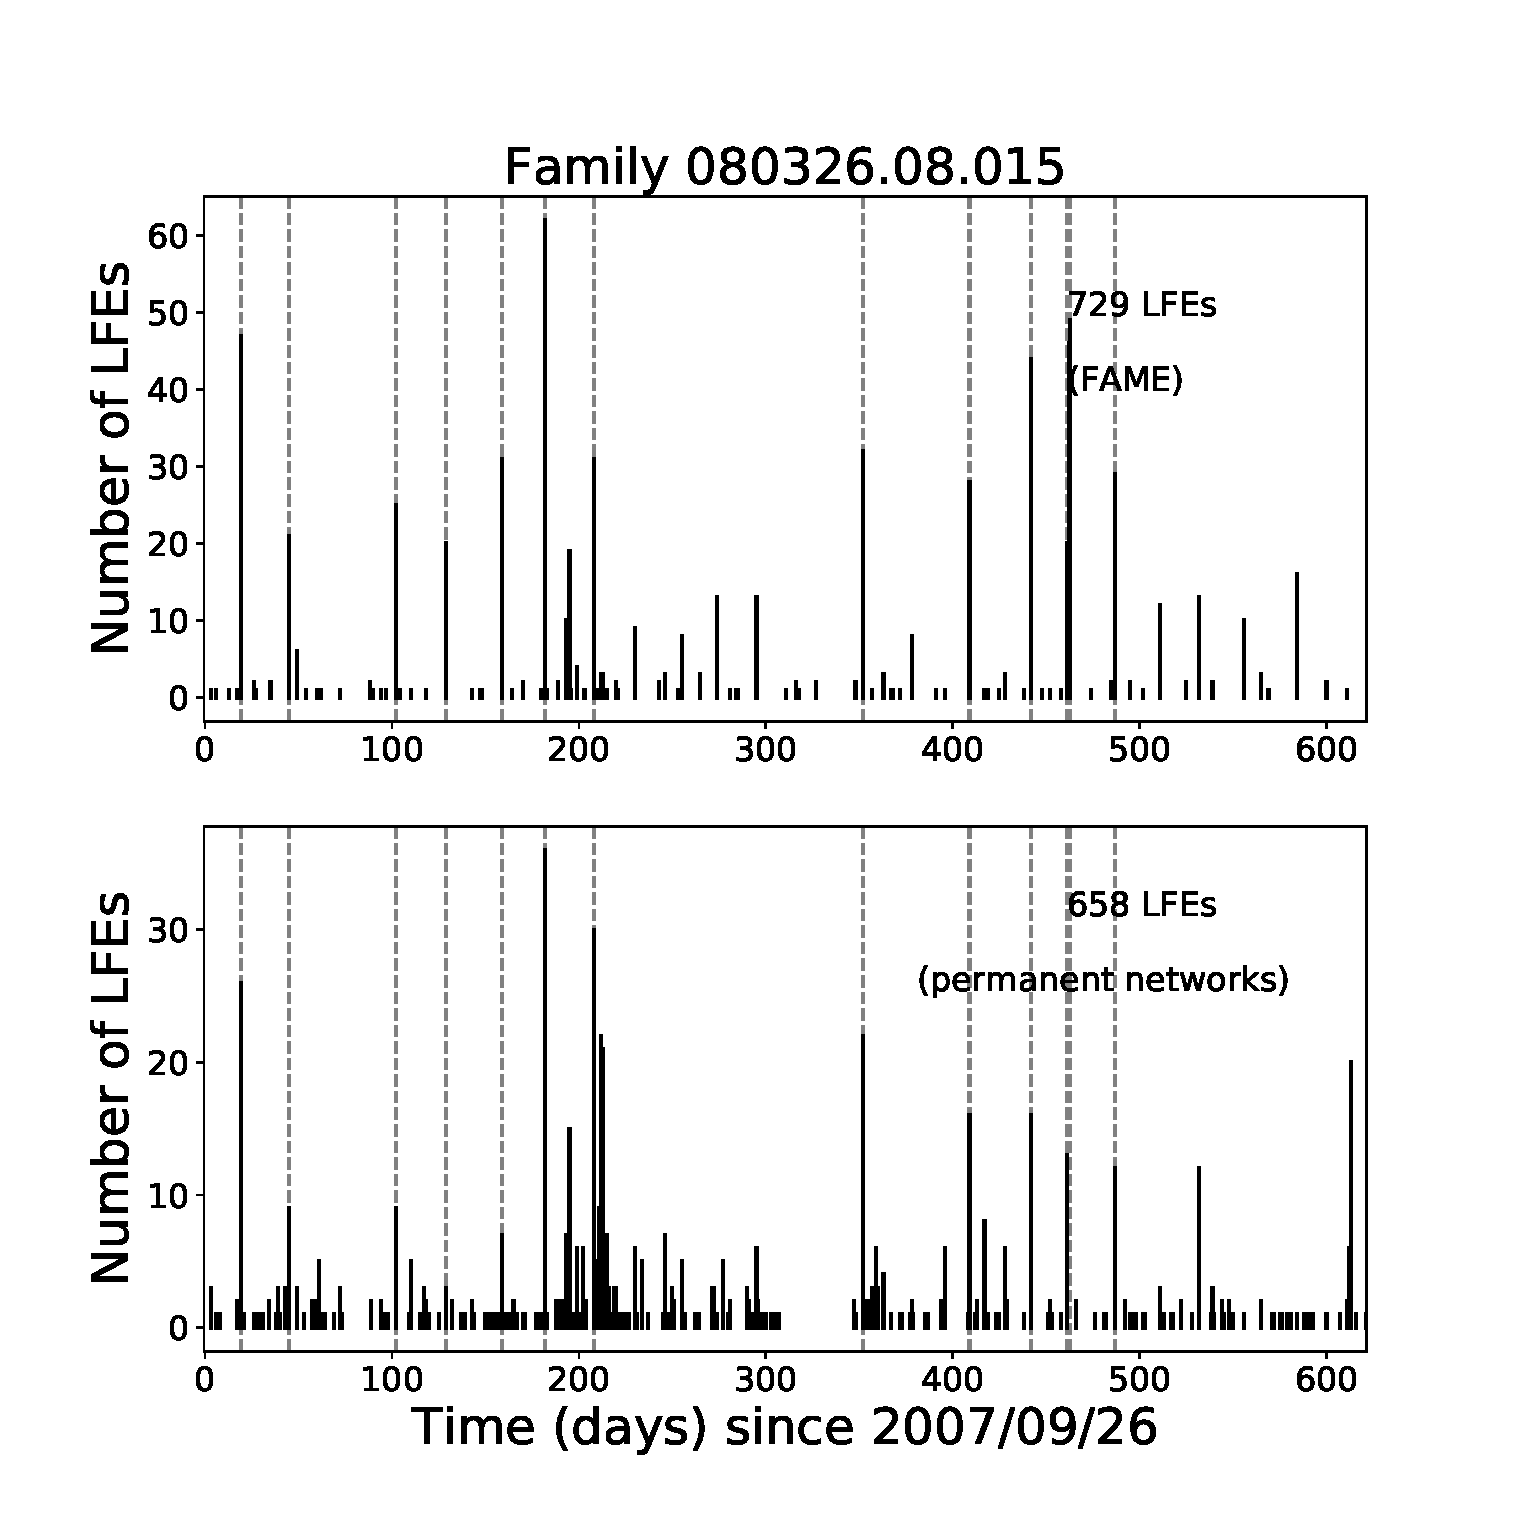
\includegraphics[width=7cm, trim={0cm 0cm 0cm 2cm}, clip]{catalog_SC/08032608015_permanent.eps}
		\end{center}
	\end{frame}

	\begin{frame}
		\frametitle{Comparison FAME - permanent networks}
		\begin{center}
			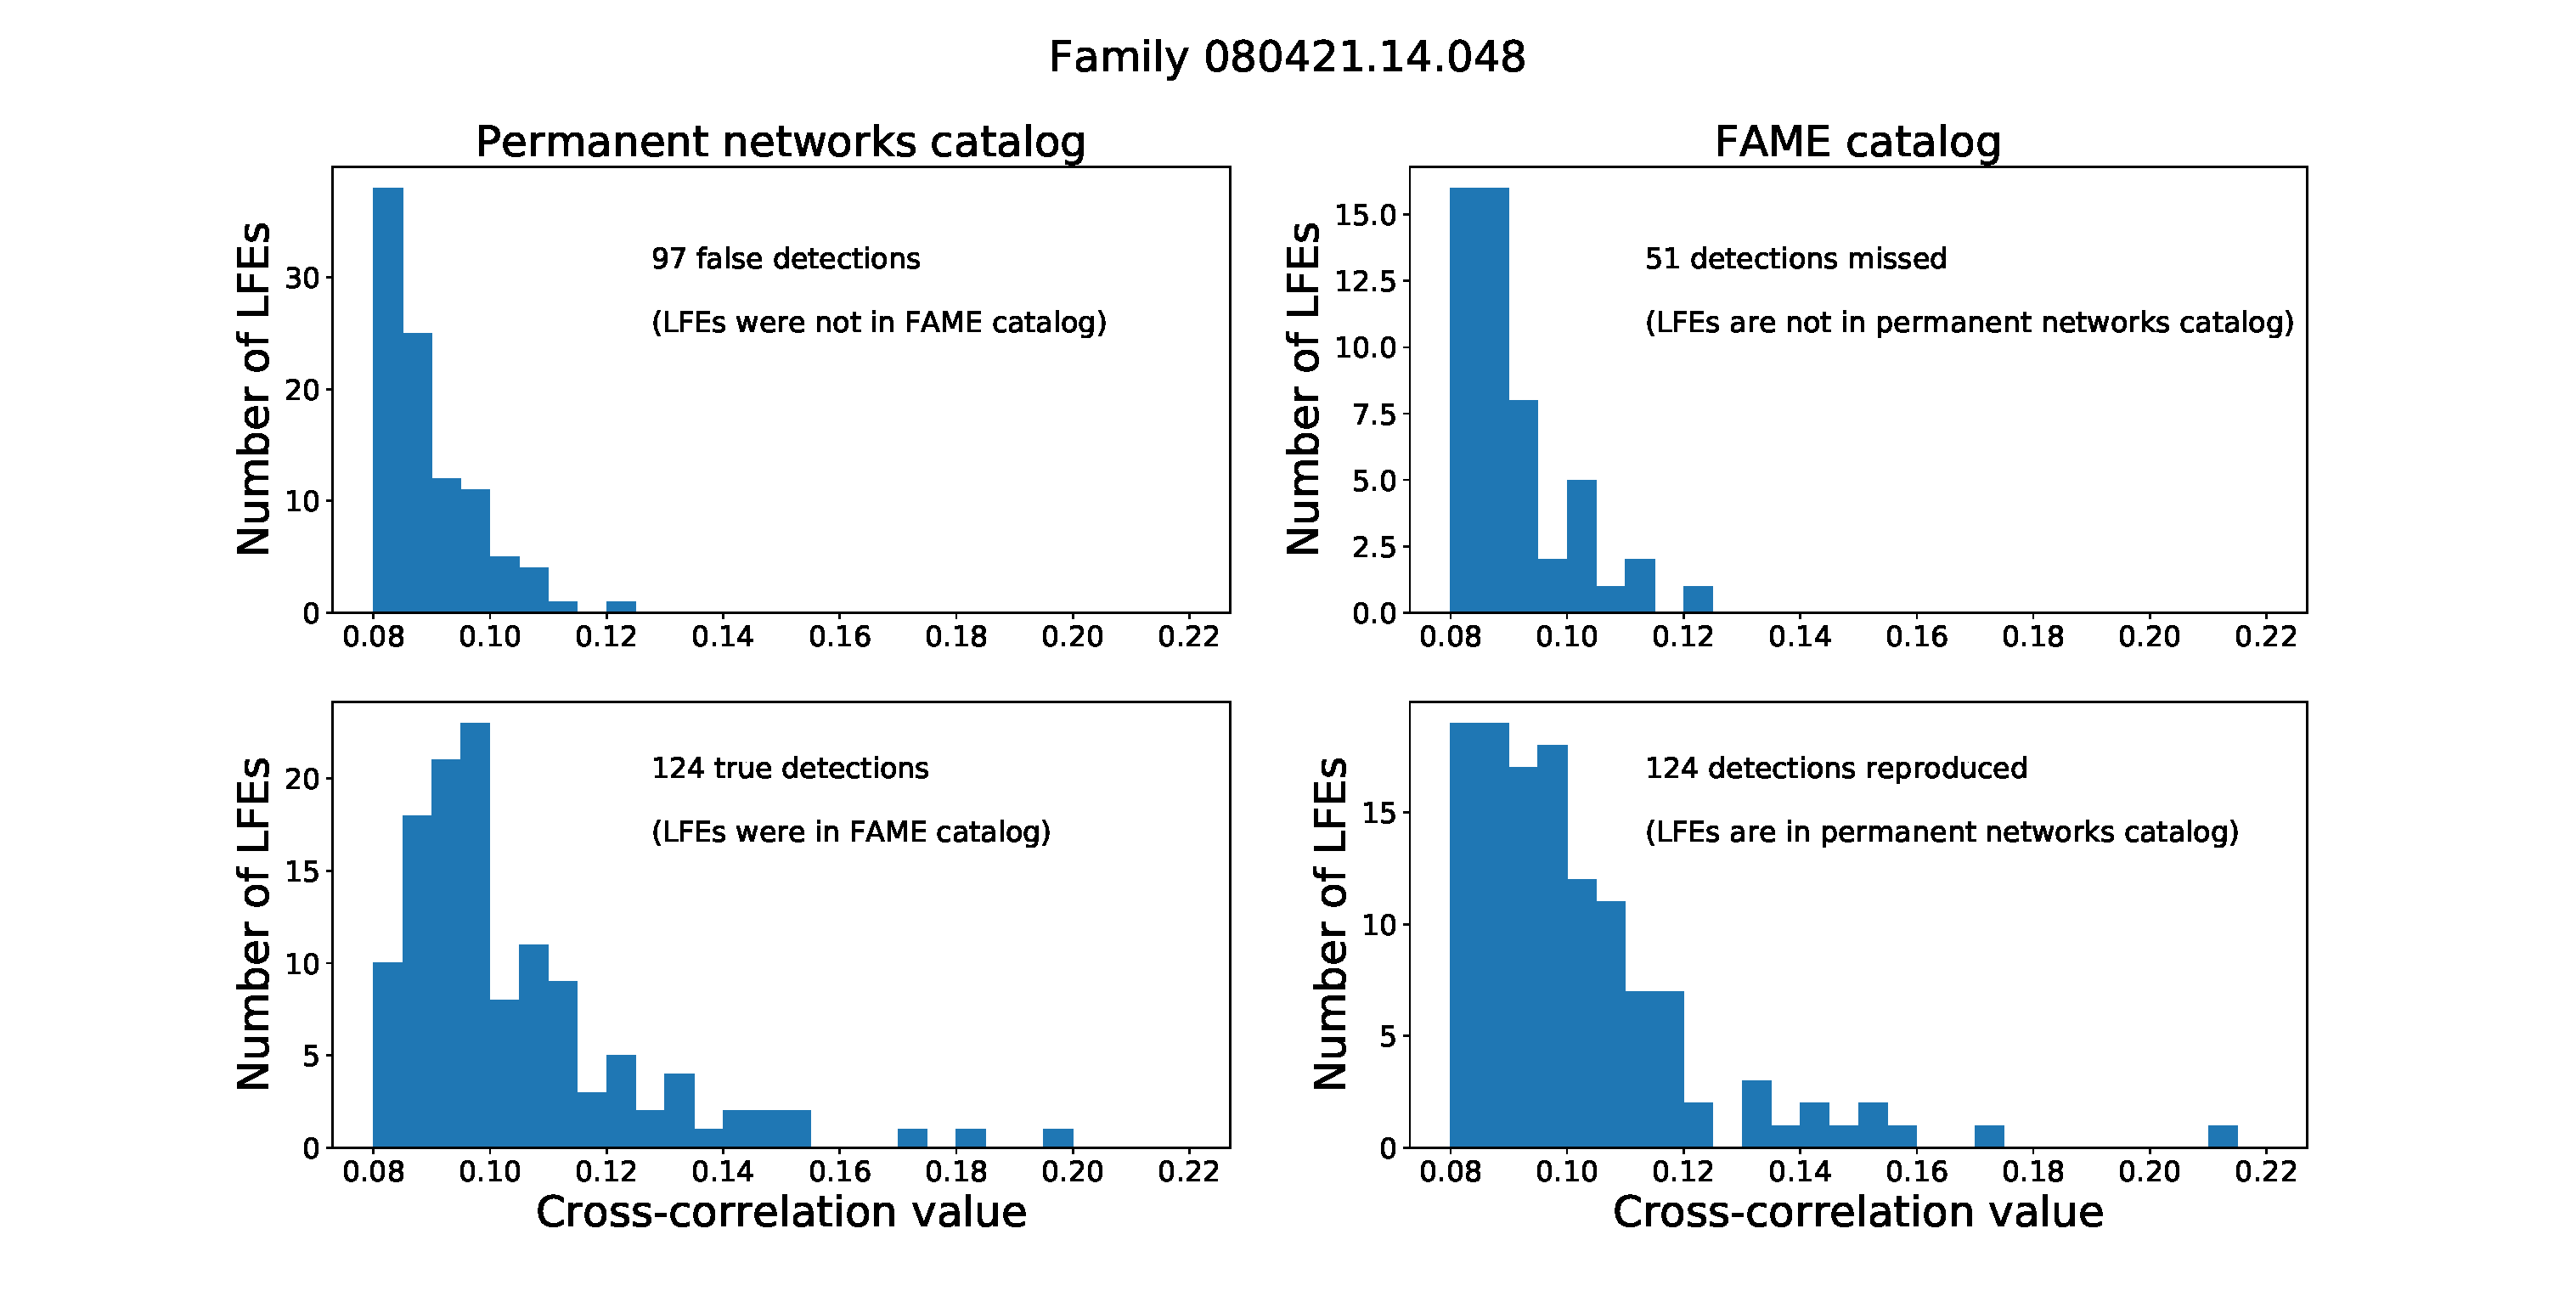
\includegraphics[width=11cm, trim={0cm 0cm 0cm 0cm}, clip]{catalog_SC/08042114048_comparison.eps}
		\end{center}
	\end{frame}

	\begin{frame}
		\frametitle{Comparison FAME - permanent networks}
		\begin{center}
			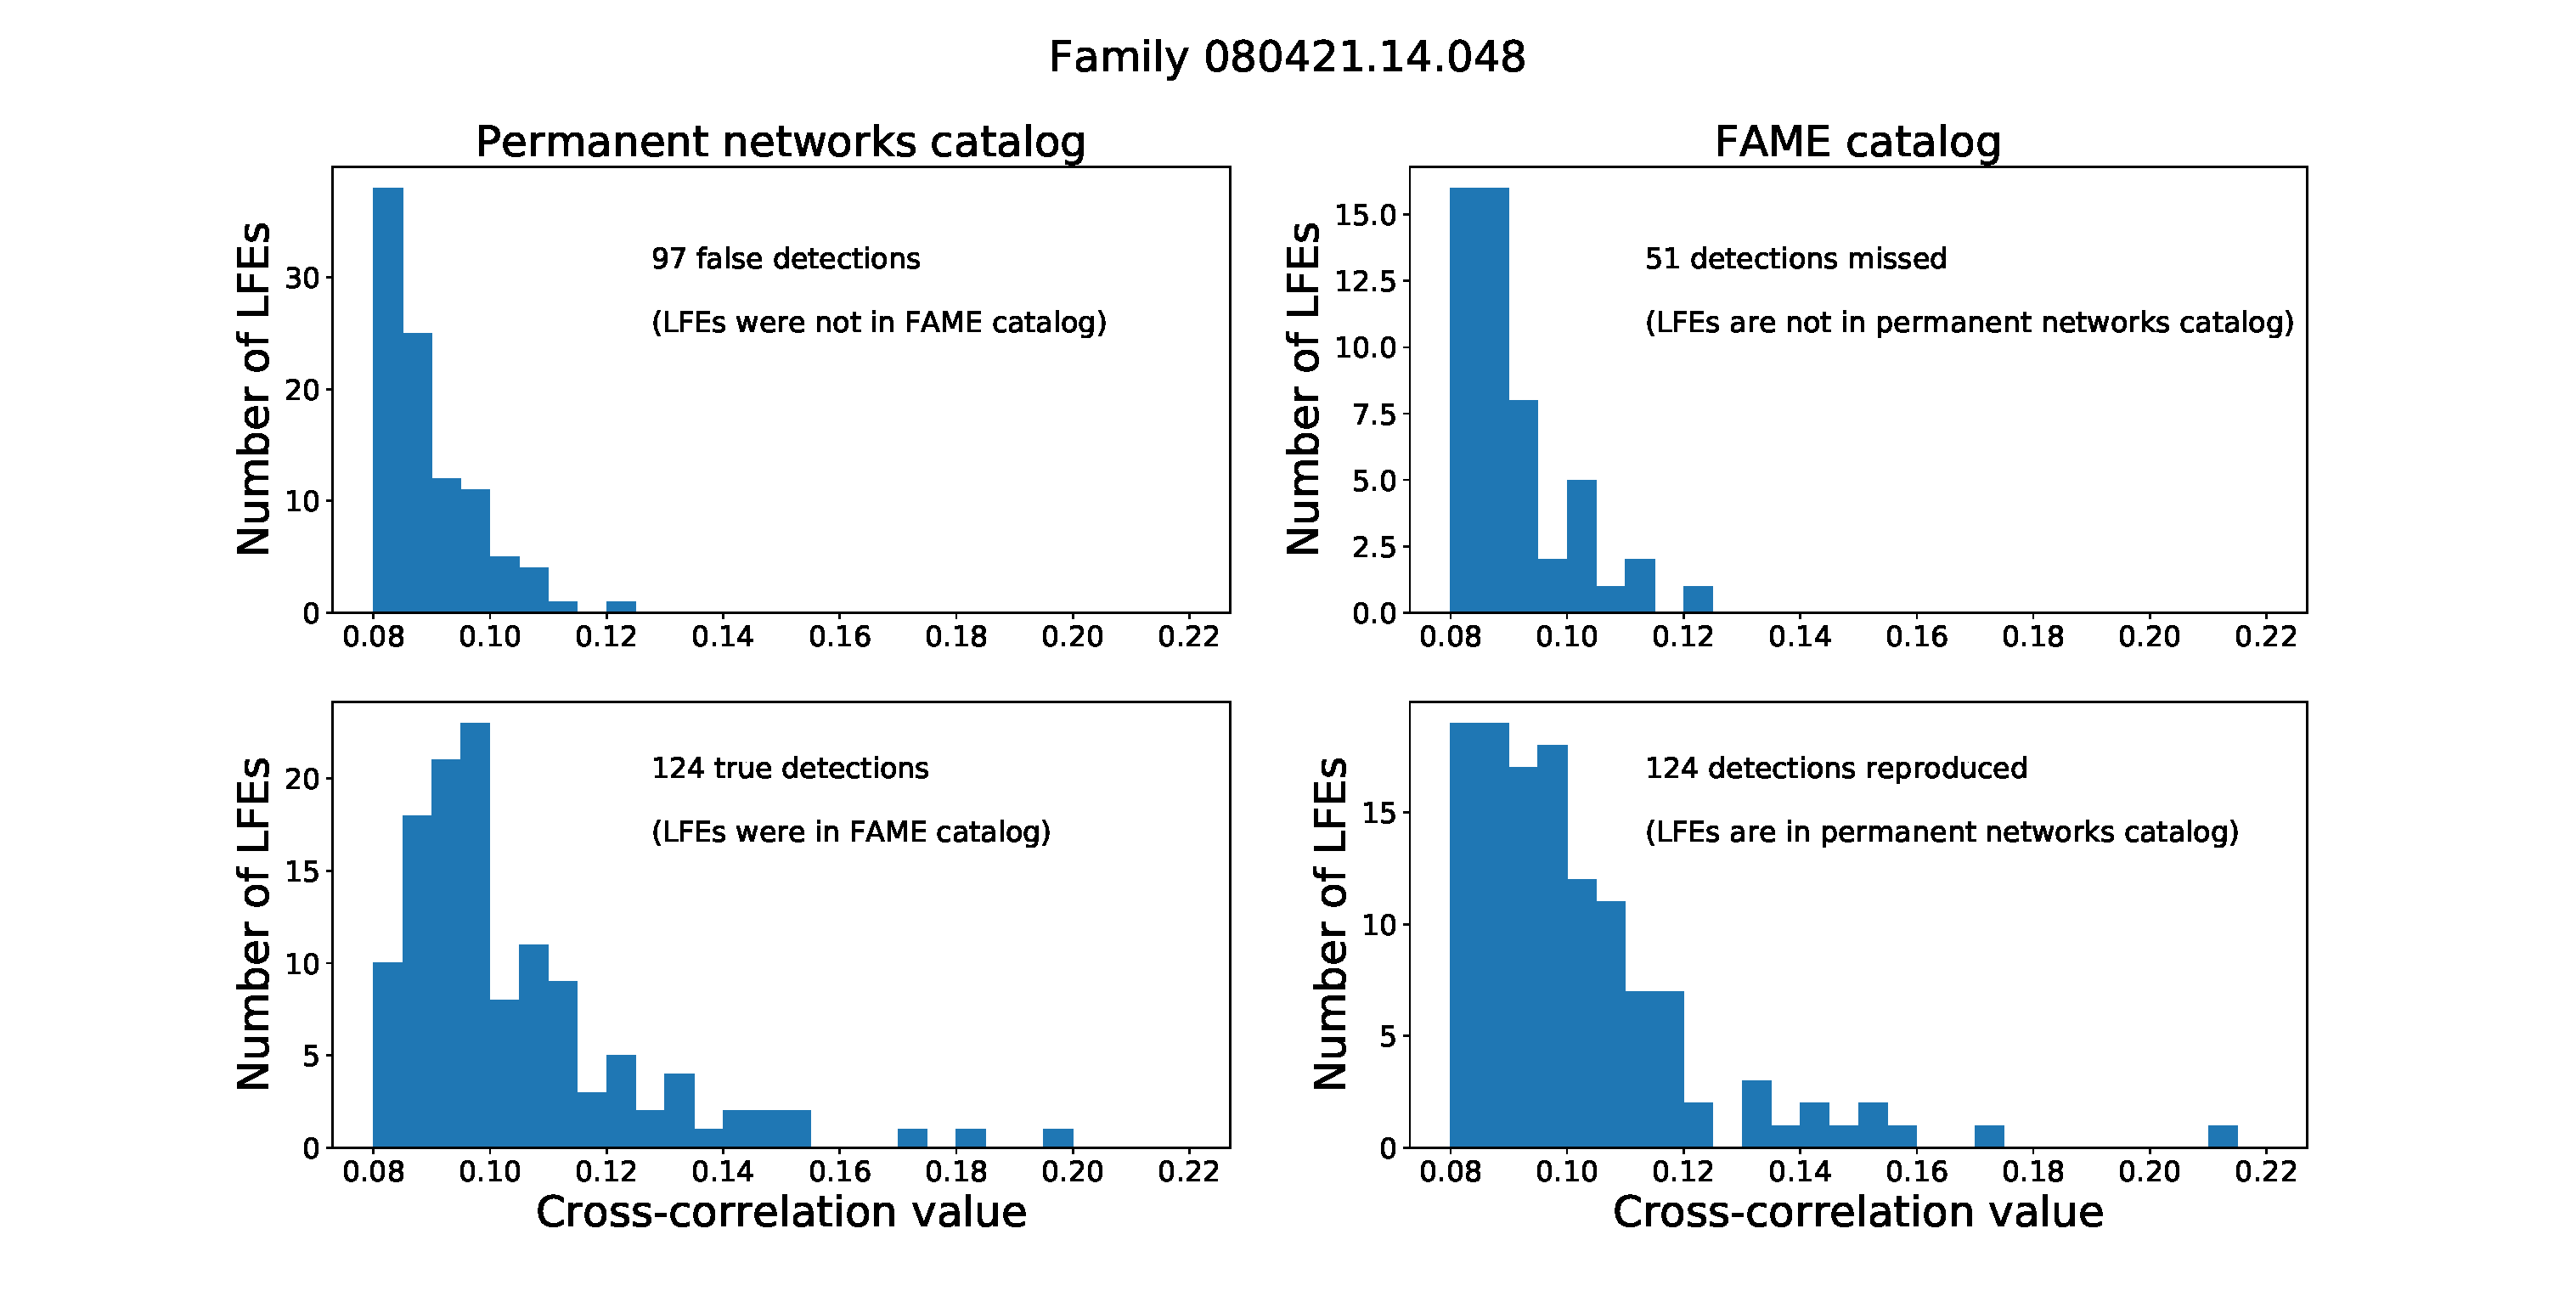
\includegraphics[width=11cm, trim={0cm 0cm 0cm 0cm}, clip]{catalog_SC/08042114048_comparison.eps}
		\end{center}
	\end{frame}

	\begin{frame}
		\frametitle{Future work}
		\begin{itemize}
			\item Two-year-long catalog for all LFE families
			\item Computation of new templates for the permanent networks
			\item Whenever possible, extension of the LFE catalog to 2009-2019
		\end{itemize}
	\end{frame}

	%----------------------------------------------------------------------------------------------------------------------------------
	% Effect of nearby earthquakes on LFE activity
	%----------------------------------------------------------------------------------------------------------------------------------

	\subsection{Effect of nearby earthquakes on LFE activity}

	\begin{frame}
		\frametitle{Effect of the 28 September 2004 M6.0 Parkfield earthquake}
		\begin{center}
			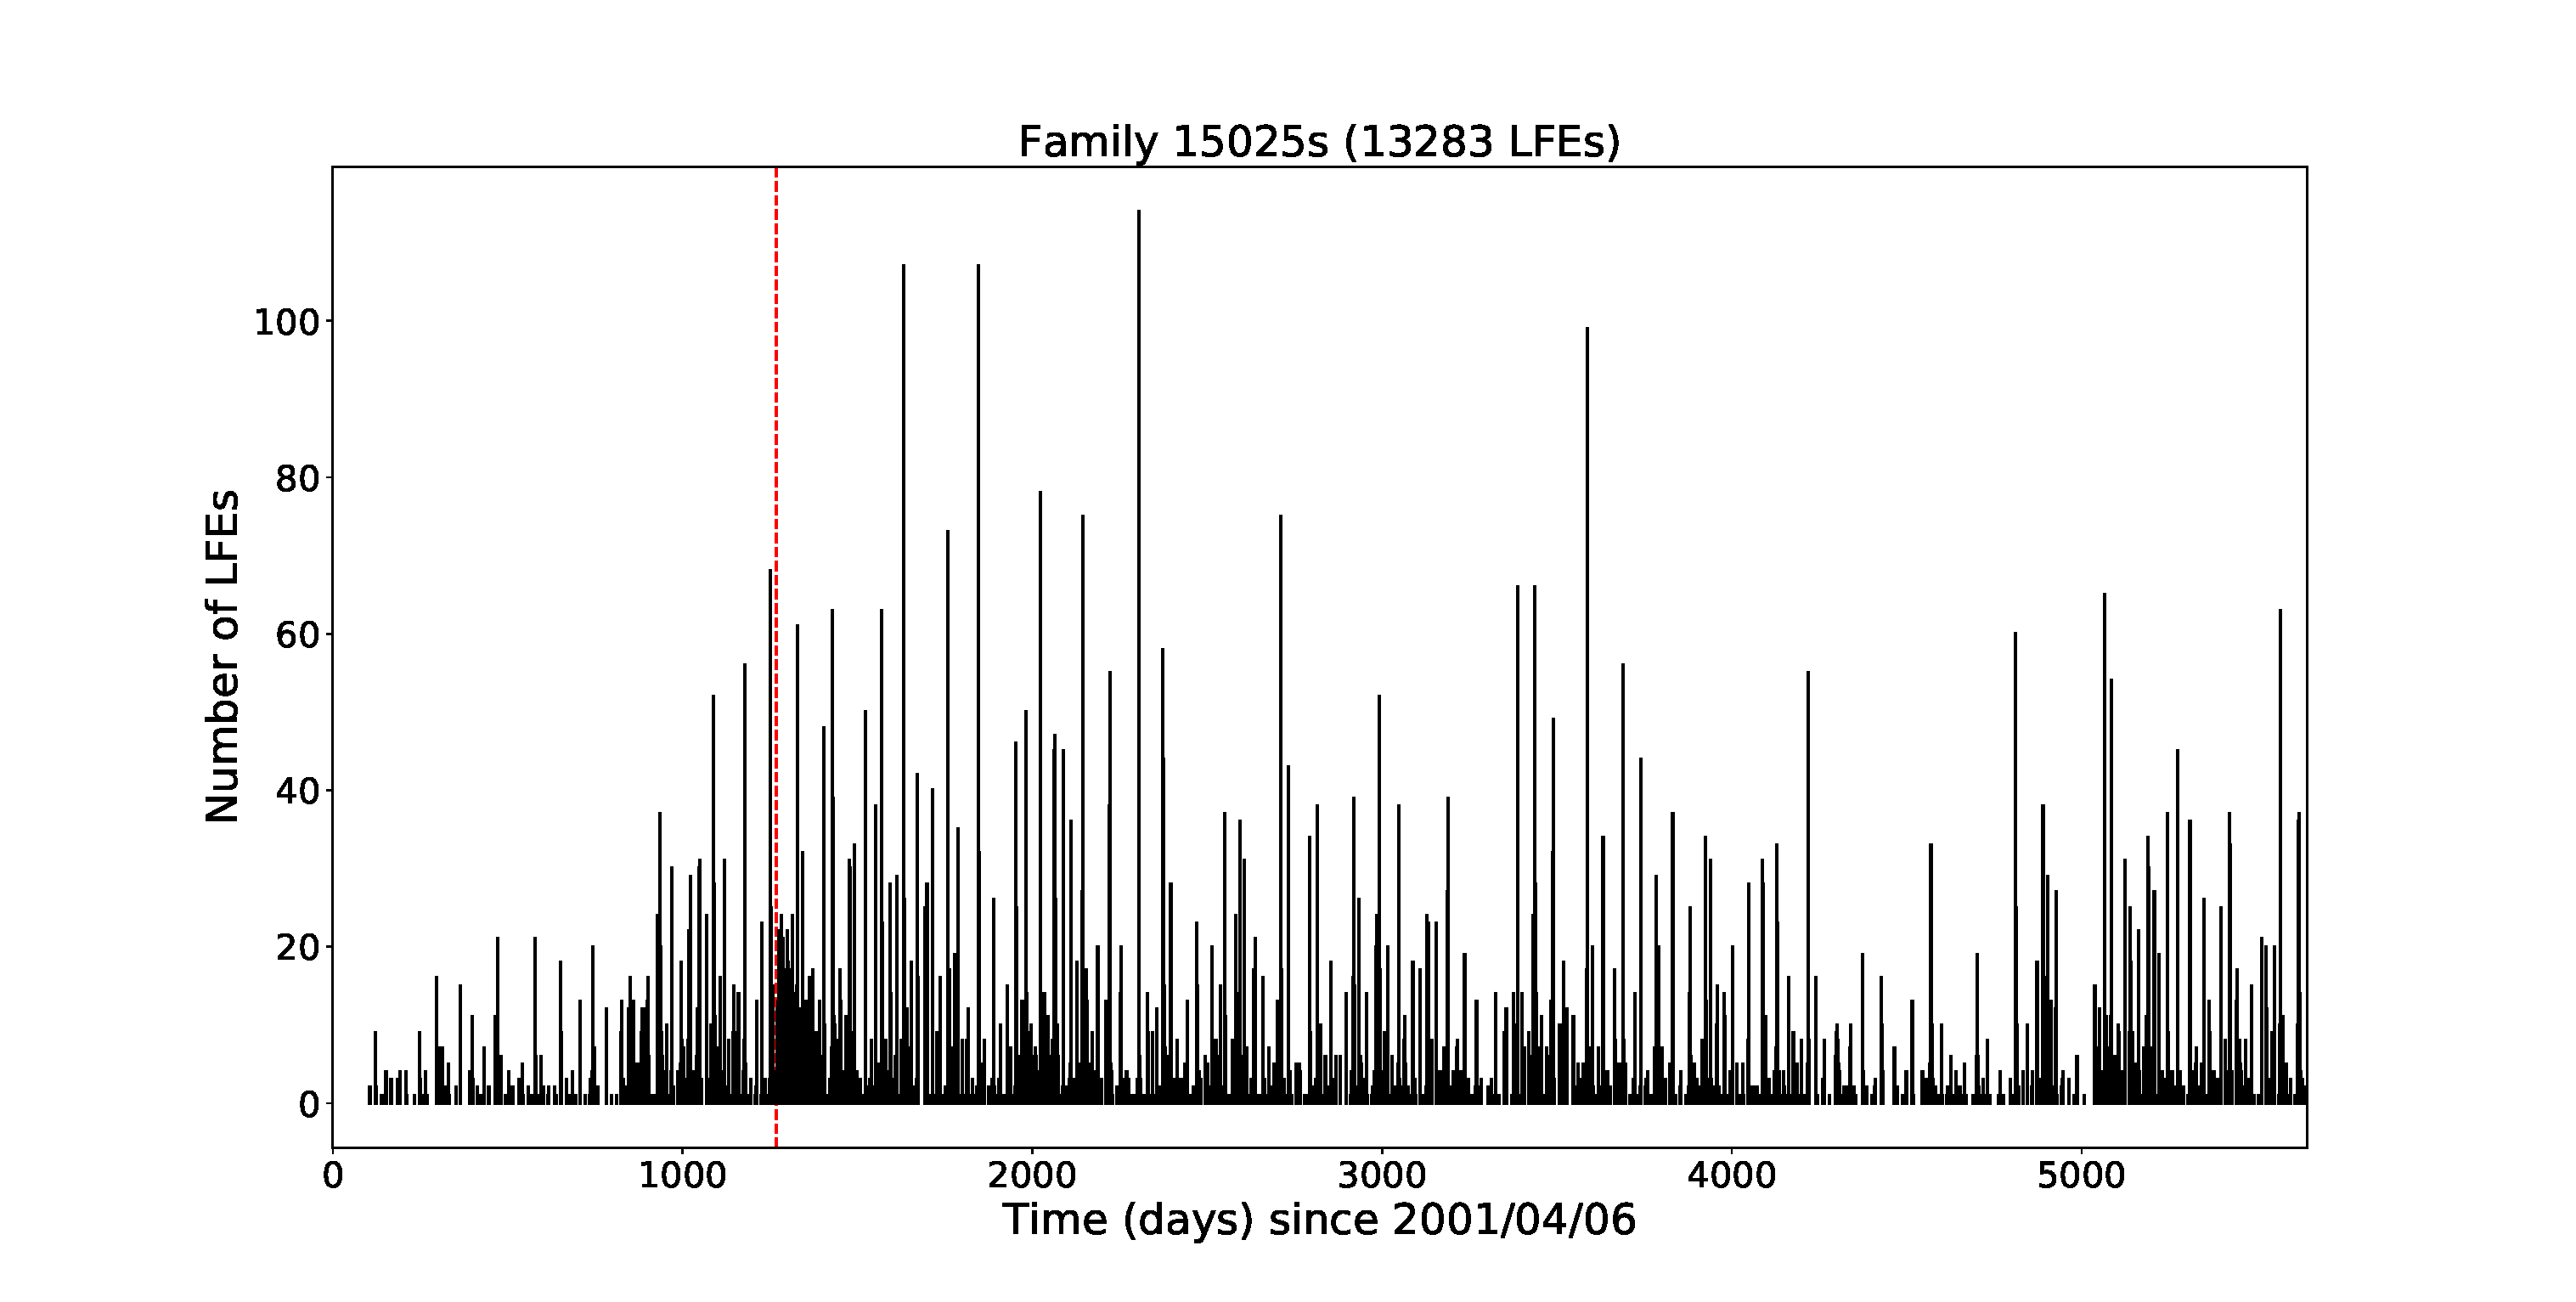
\includegraphics[width=11cm, trim={0cm 0cm 0cm 0cm}, clip]{LFE_catalogs/15025s_Parkfield.eps}
		\end{center}
	\end{frame}

	\begin{frame}
		\frametitle{Effect of the 28 September 2004 M6.0 Parkfield earthquake}
		\begin{center}
			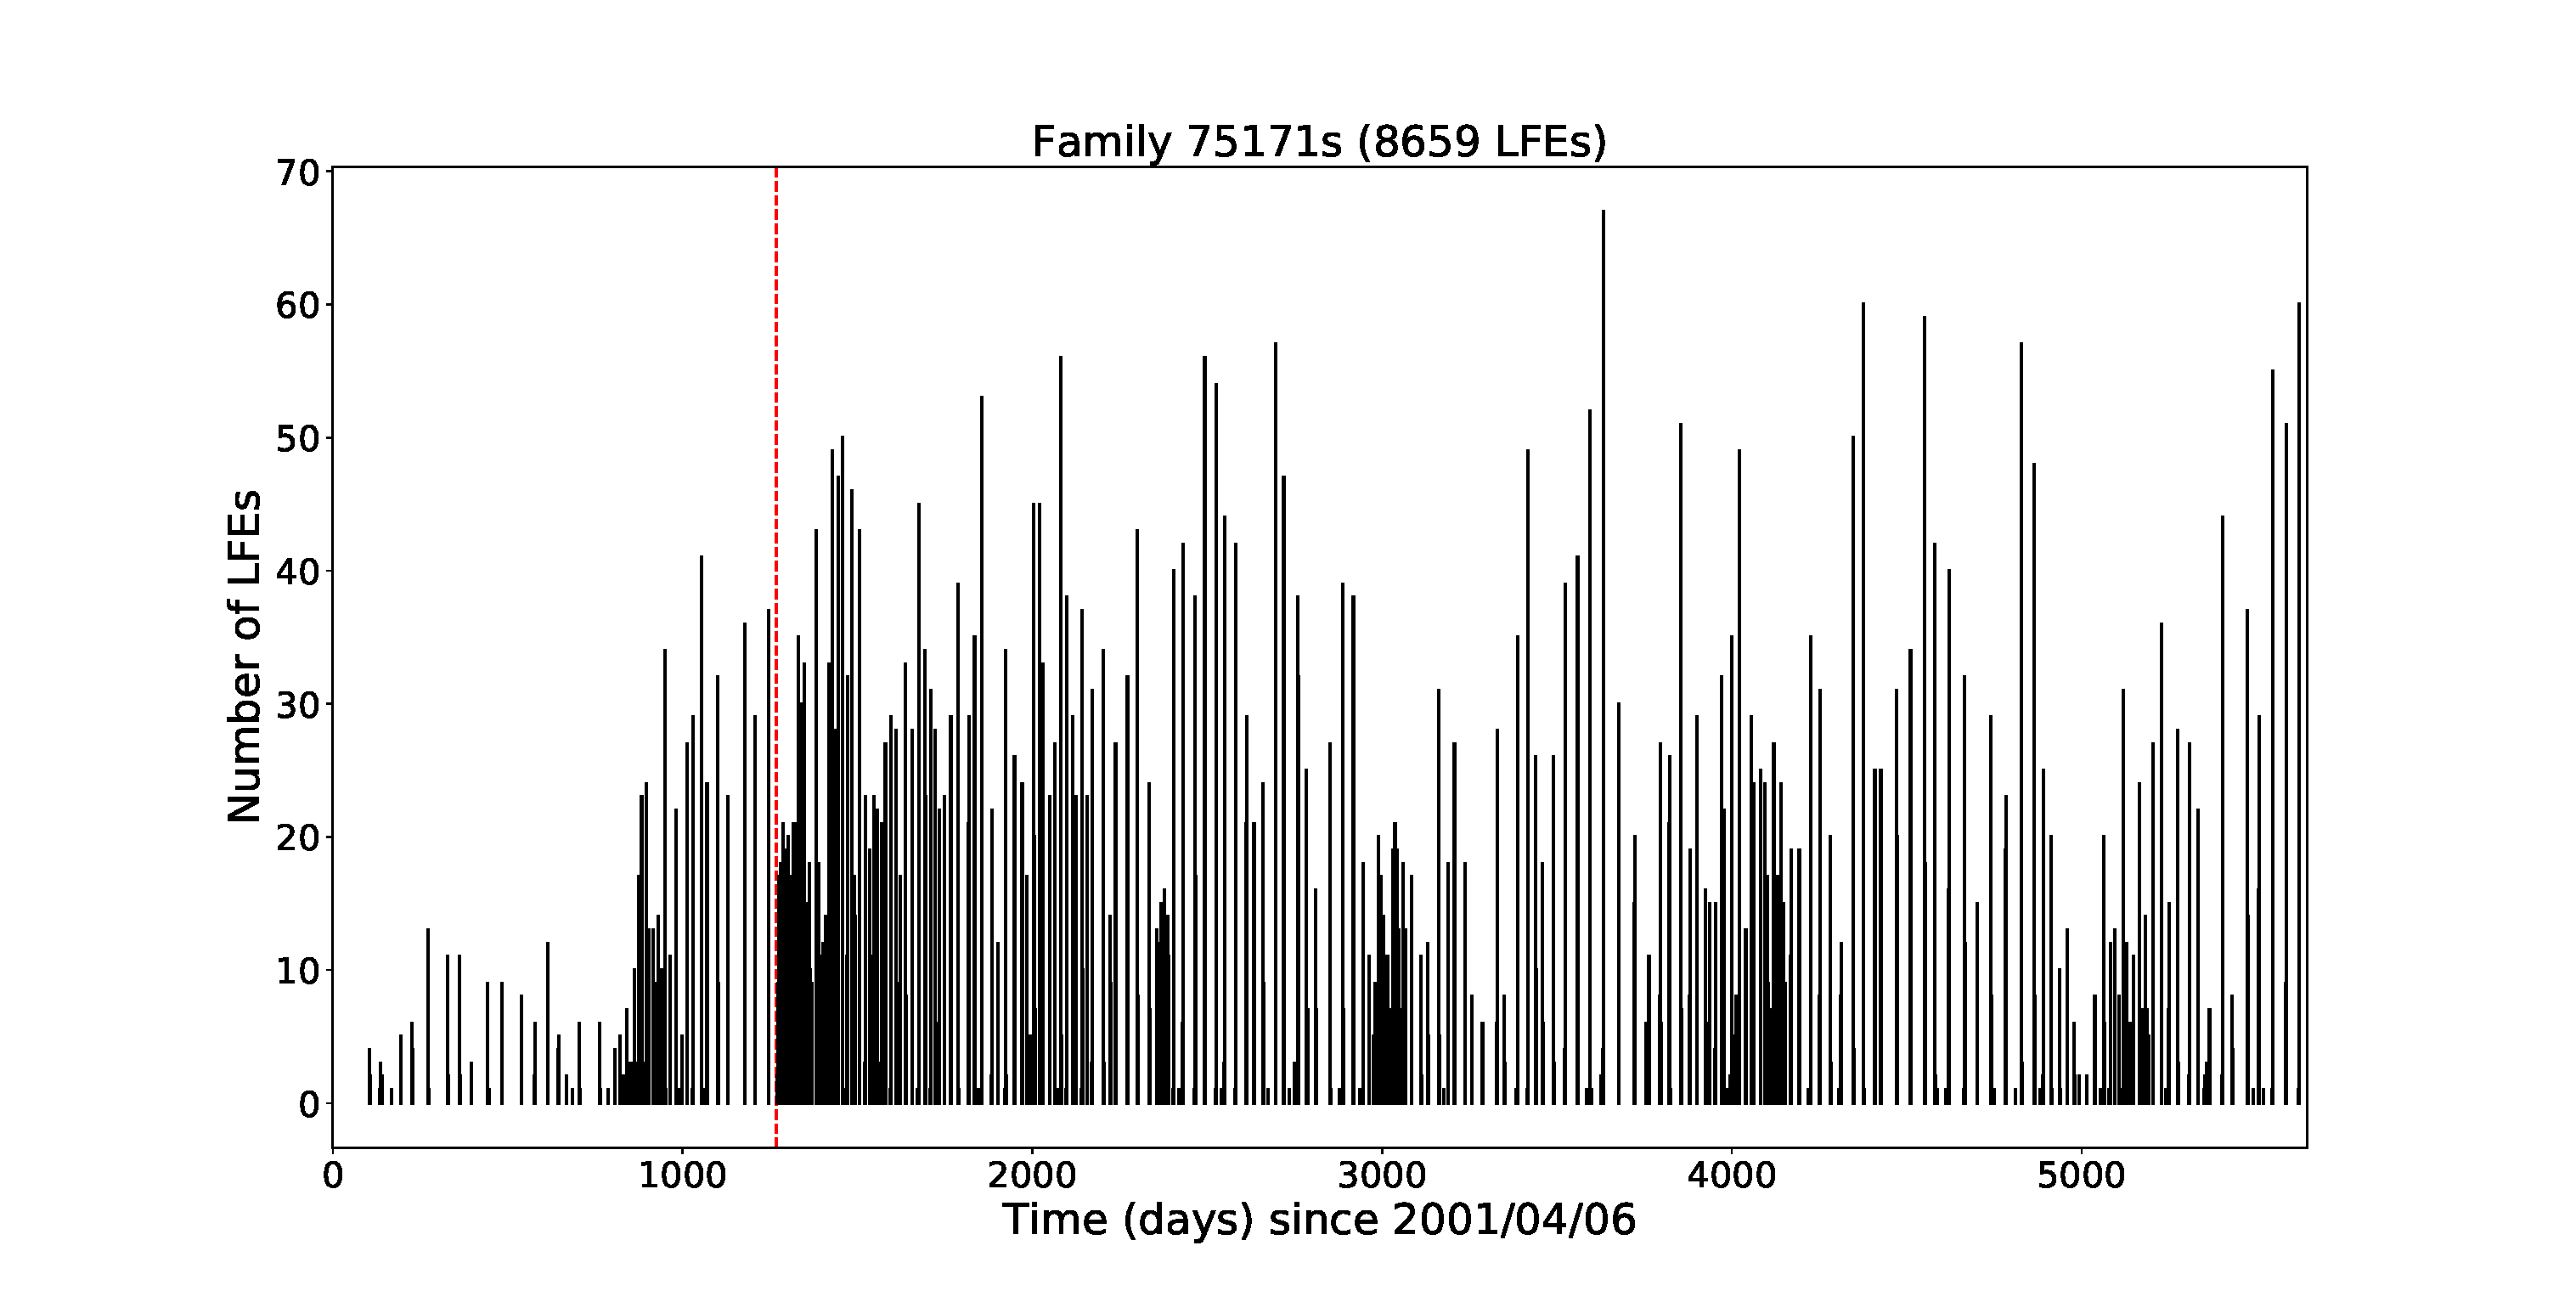
\includegraphics[width=11cm, trim={0cm 0cm 0cm 0cm}, clip]{LFE_catalogs/75171s_Parkfield.eps}
		\end{center}
	\end{frame}

	\begin{frame}
		\frametitle{Moderate earthquakes in southern Cascadia}
		\begin{center}
			\includegraphics[trim={1cm 4cm 1cm 10cm}, clip, width=8cm]{catalog_SC/earthquakes_map.eps}
		\end{center}
	\end{frame}

	\begin{frame}
		\frametitle{Future work}
		\begin{itemize}
			\item Event rate before the earthquake
			\item Event rate after the earthquake
			\item Comparison between two event rates: Computation of likelihood ratio
		\end{itemize}
	\end{frame}

	%----------------------------------------------------------------------------------------------------------------------------------
	% Characterization of LFE clustering
	%----------------------------------------------------------------------------------------------------------------------------------

	\subsection{Characterization of LFE clustering}

	\begin{frame}
		\frametitle{Long-range dependence}
		\begin{itemize}
			\item Relates to the slow rate of decay of the statistical dependence between two points with increasing time interval between the points
			\item The fractional index $d$ represents how fast the variance in the number of LFEs in a time window of a given length increases with the length of the time window considered
			\item $0 < d < 0.5$ is characteristic of long-range dependence
		\end{itemize}
	\end{frame}

	\begin{frame}
		\frametitle{Homogeneous Poisson process}
		\begin{center}
			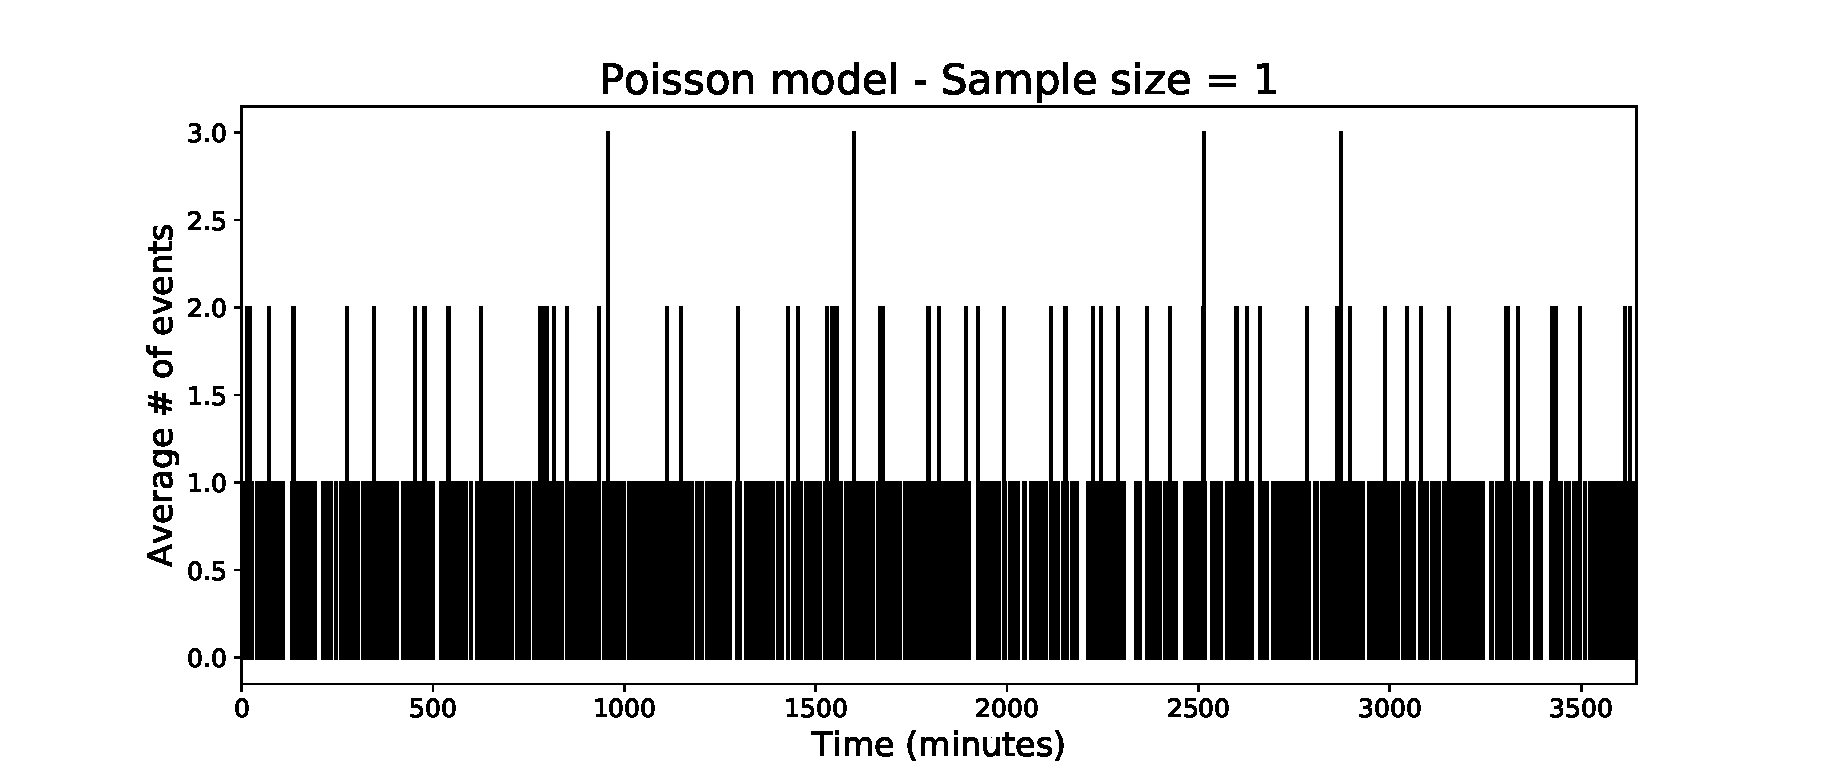
\includegraphics[width=9cm, trim={1cm 0cm 3cm 0cm}, clip]{longrange/Poisson_1.eps}
		\end{center}
		Number of events recorded during one day

		$\rightarrow$ Variance over 3645 values = $0.206$
	\end{frame}

	\begin{frame}
		\frametitle{Homogeneous Poisson process}
		\begin{center}
			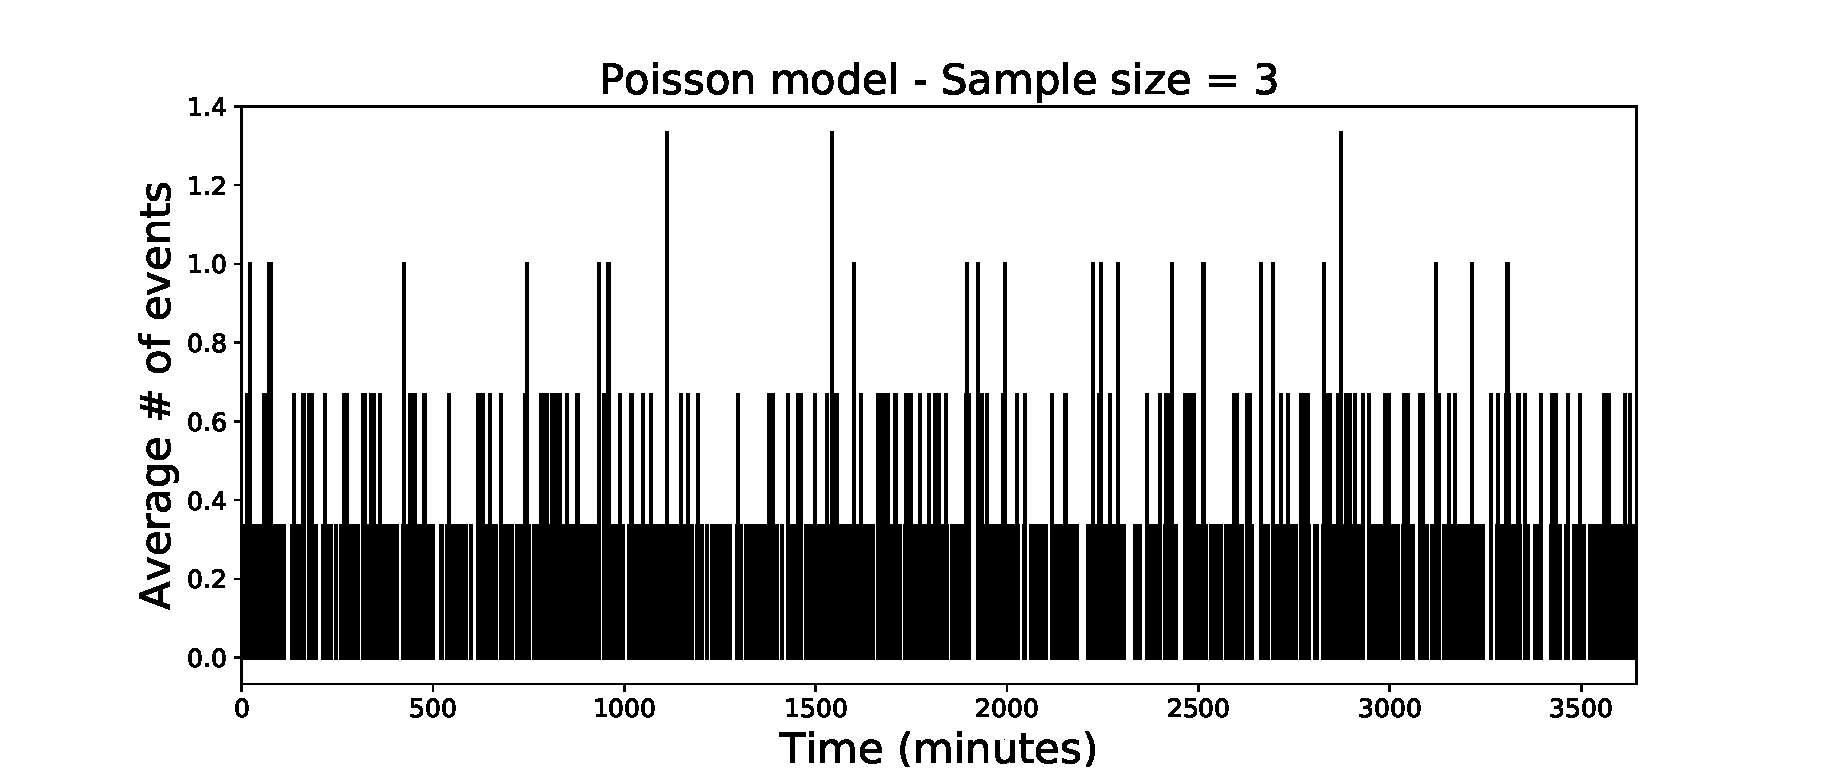
\includegraphics[width=9cm, trim={1cm 0cm 3cm 0cm}, clip]{longrange/Poisson_2.eps}
		\end{center}
		Number of events recorded during 3 days

		$\rightarrow$ Variance over 1215 values = $6.62 10^{-2}$
	\end{frame}

	\begin{frame}
		\frametitle{Homogeneous Poisson process}
		\begin{center}
			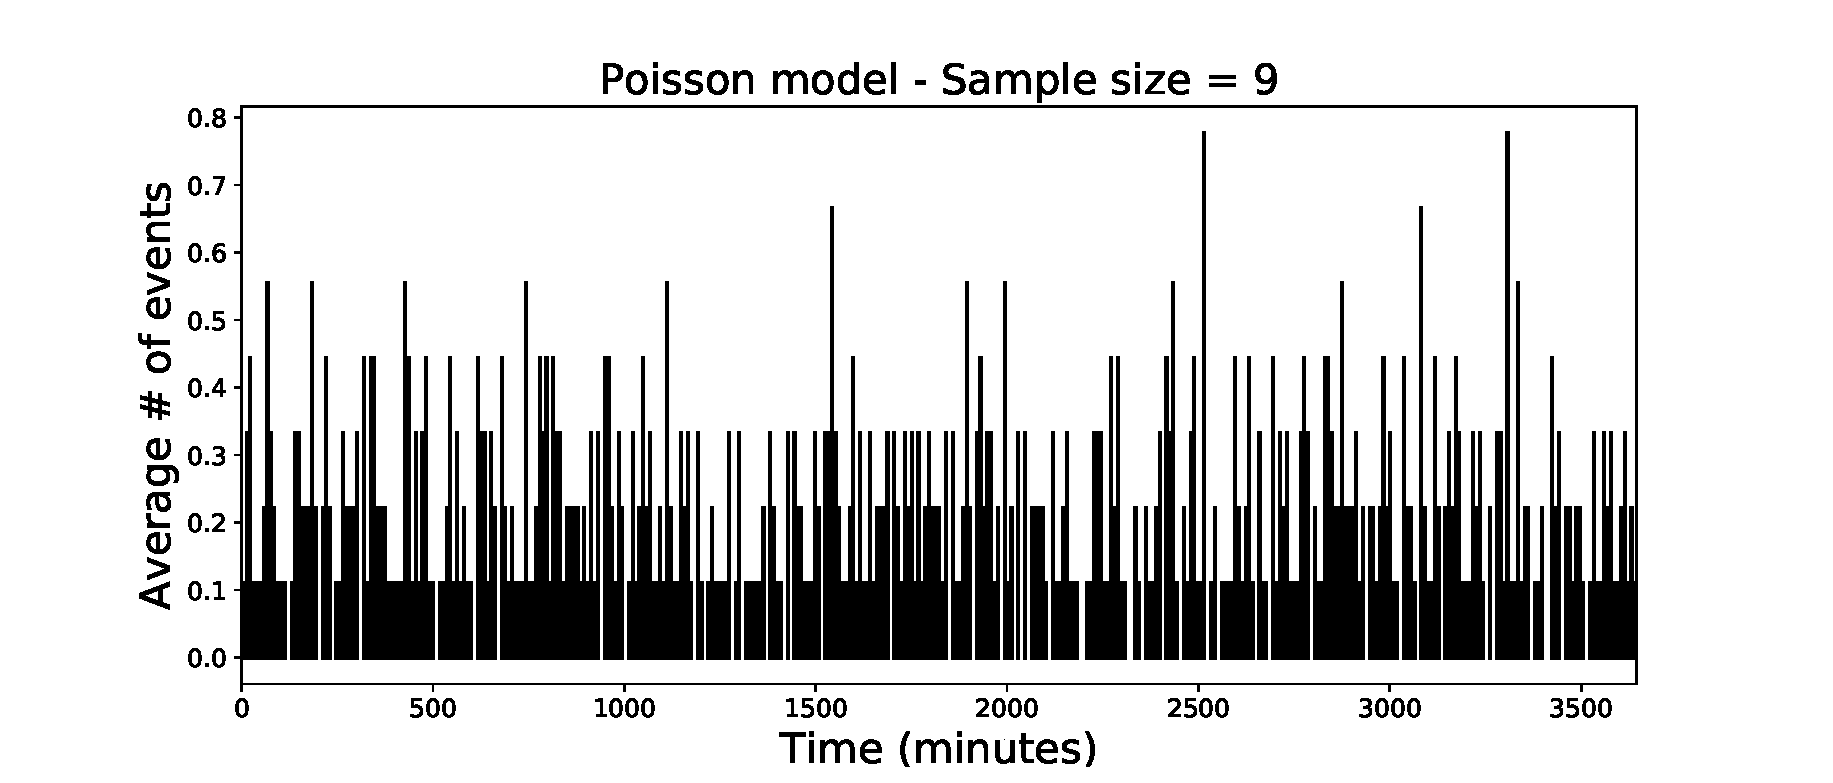
\includegraphics[width=9cm, trim={1cm 0cm 3cm 0cm}, clip]{longrange/Poisson_3.eps}
		\end{center}
		Number of events recorded during 9 days

		$\rightarrow$ Variance over 405 values = $2.14 10^{-2}$
	\end{frame}

	\begin{frame}
		\frametitle{Homogeneous Poisson process}
		\begin{center}
			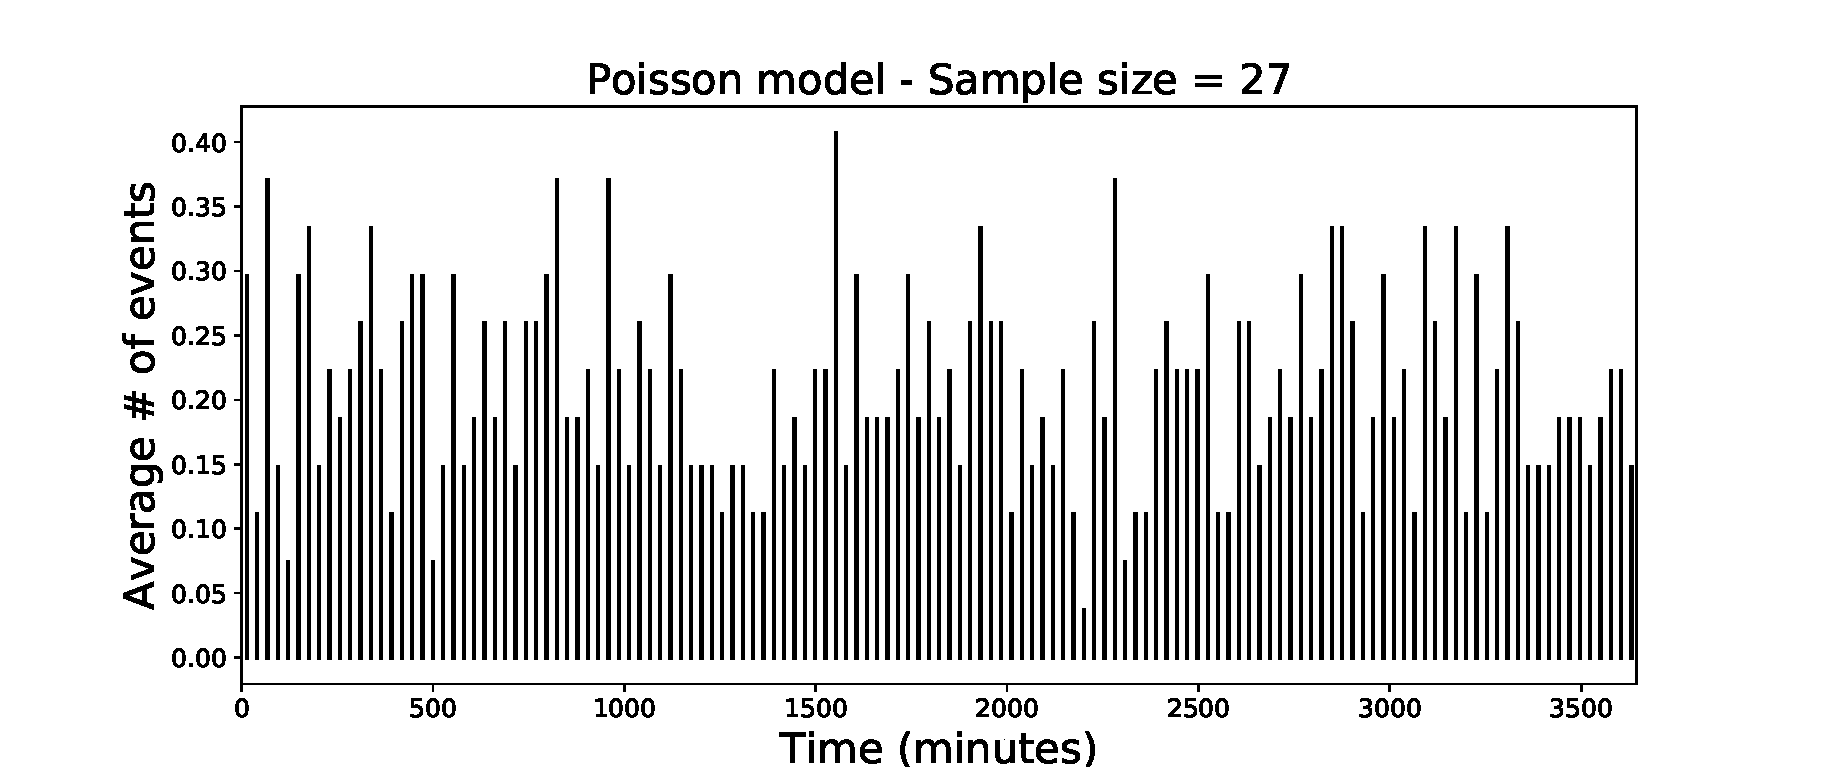
\includegraphics[width=9cm, trim={1cm 0cm 3cm 0cm}, clip]{longrange/Poisson_4.eps}
		\end{center}
		Number of events recorded during 27 days

		$\rightarrow$ Variance over 135 values = $5.56 10^{-3}$
	\end{frame}

	\begin{frame}
		\frametitle{Homogeneous Poisson process}
		\begin{center}
			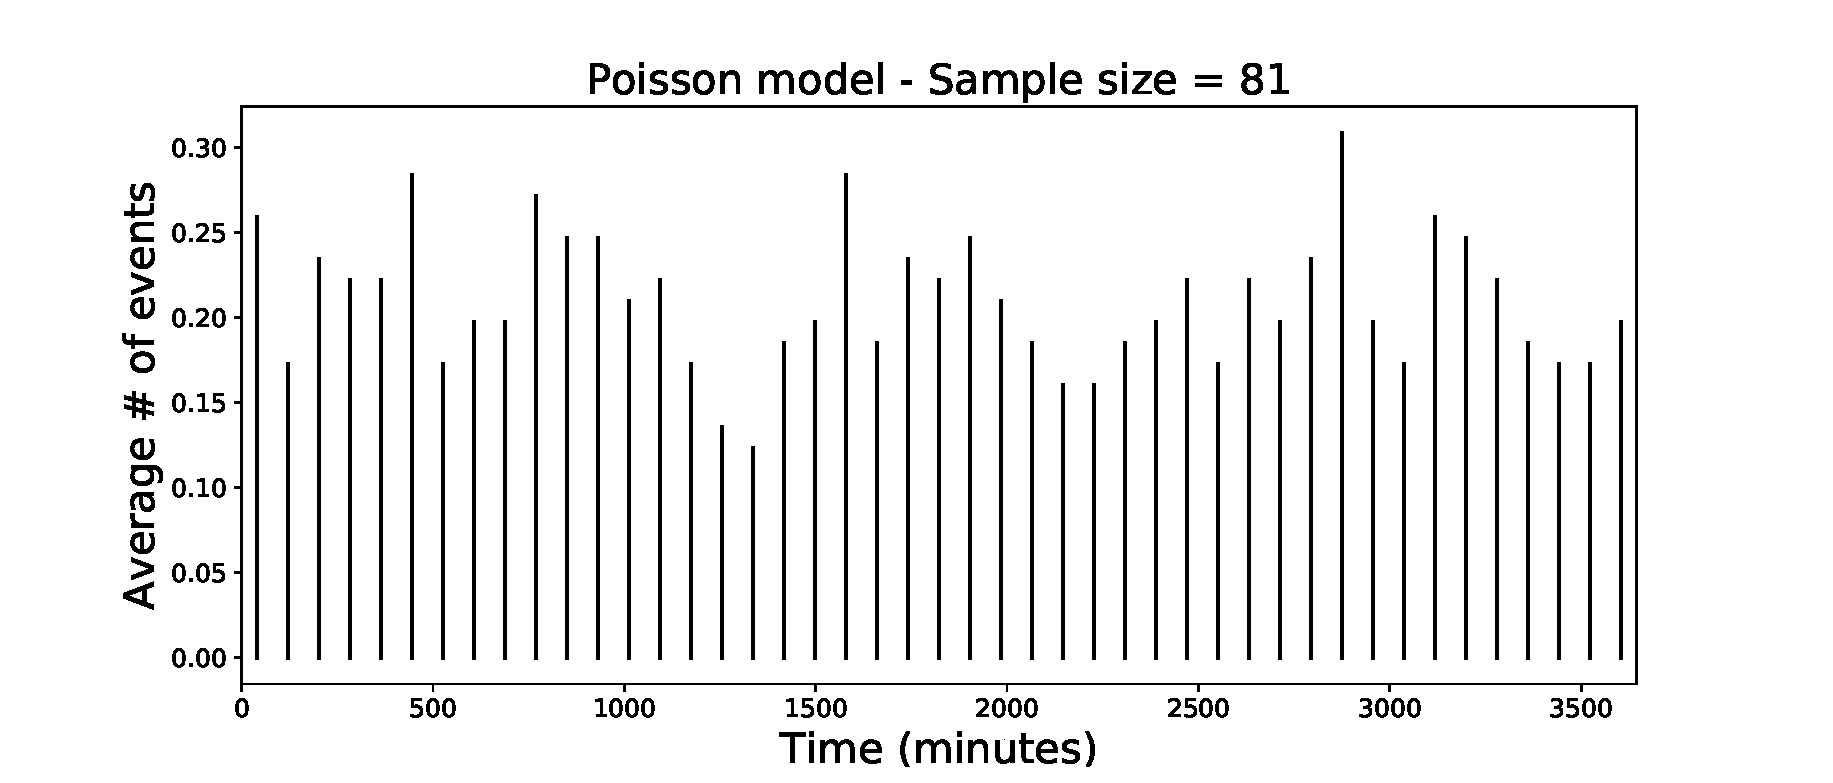
\includegraphics[width=9cm, trim={1cm 0cm 3cm 0cm}, clip]{longrange/Poisson_5.eps}
		\end{center}
		Number of events recorded during 81 days

		$\rightarrow$ Variance over 45 values = $1.54 10^{-3}$
	\end{frame}

	\begin{frame}
		\frametitle{Homogeneous Poisson process}
		\begin{center}
			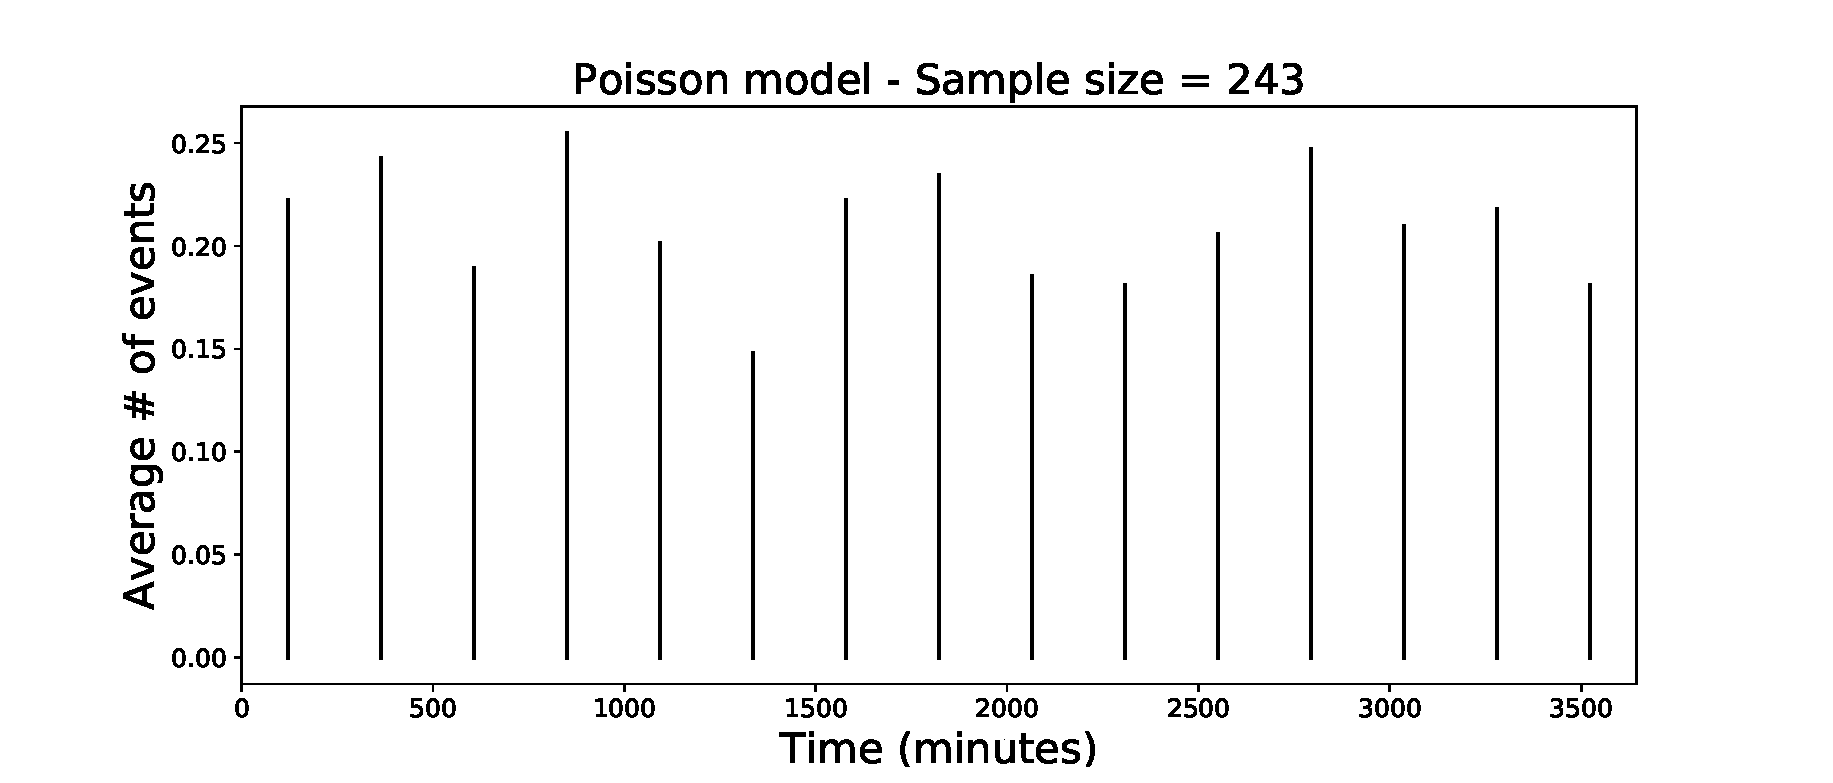
\includegraphics[width=9cm, trim={1cm 0cm 3cm 0cm}, clip]{longrange/Poisson_6.eps}
		\end{center}
		Number of events recorded during 243 days

		$\rightarrow$ Variance over 15 values = $8.05 10^{-4}$
	\end{frame}

	\begin{frame}
		\frametitle{Variance vs Length of time window}
		\begin{columns}[c]
			\begin{column}{4cm}
				$V$ = Variance

				\vspace{1em}

				$m$ = Sample size

				\vspace{1em}

				$V$ behaves as $m^{2 d - 1}$

				\vspace{1em}

				$\rightarrow$ $d =  0$
			\end{column}
			\begin{column}{7cm}
				\begin{center}
					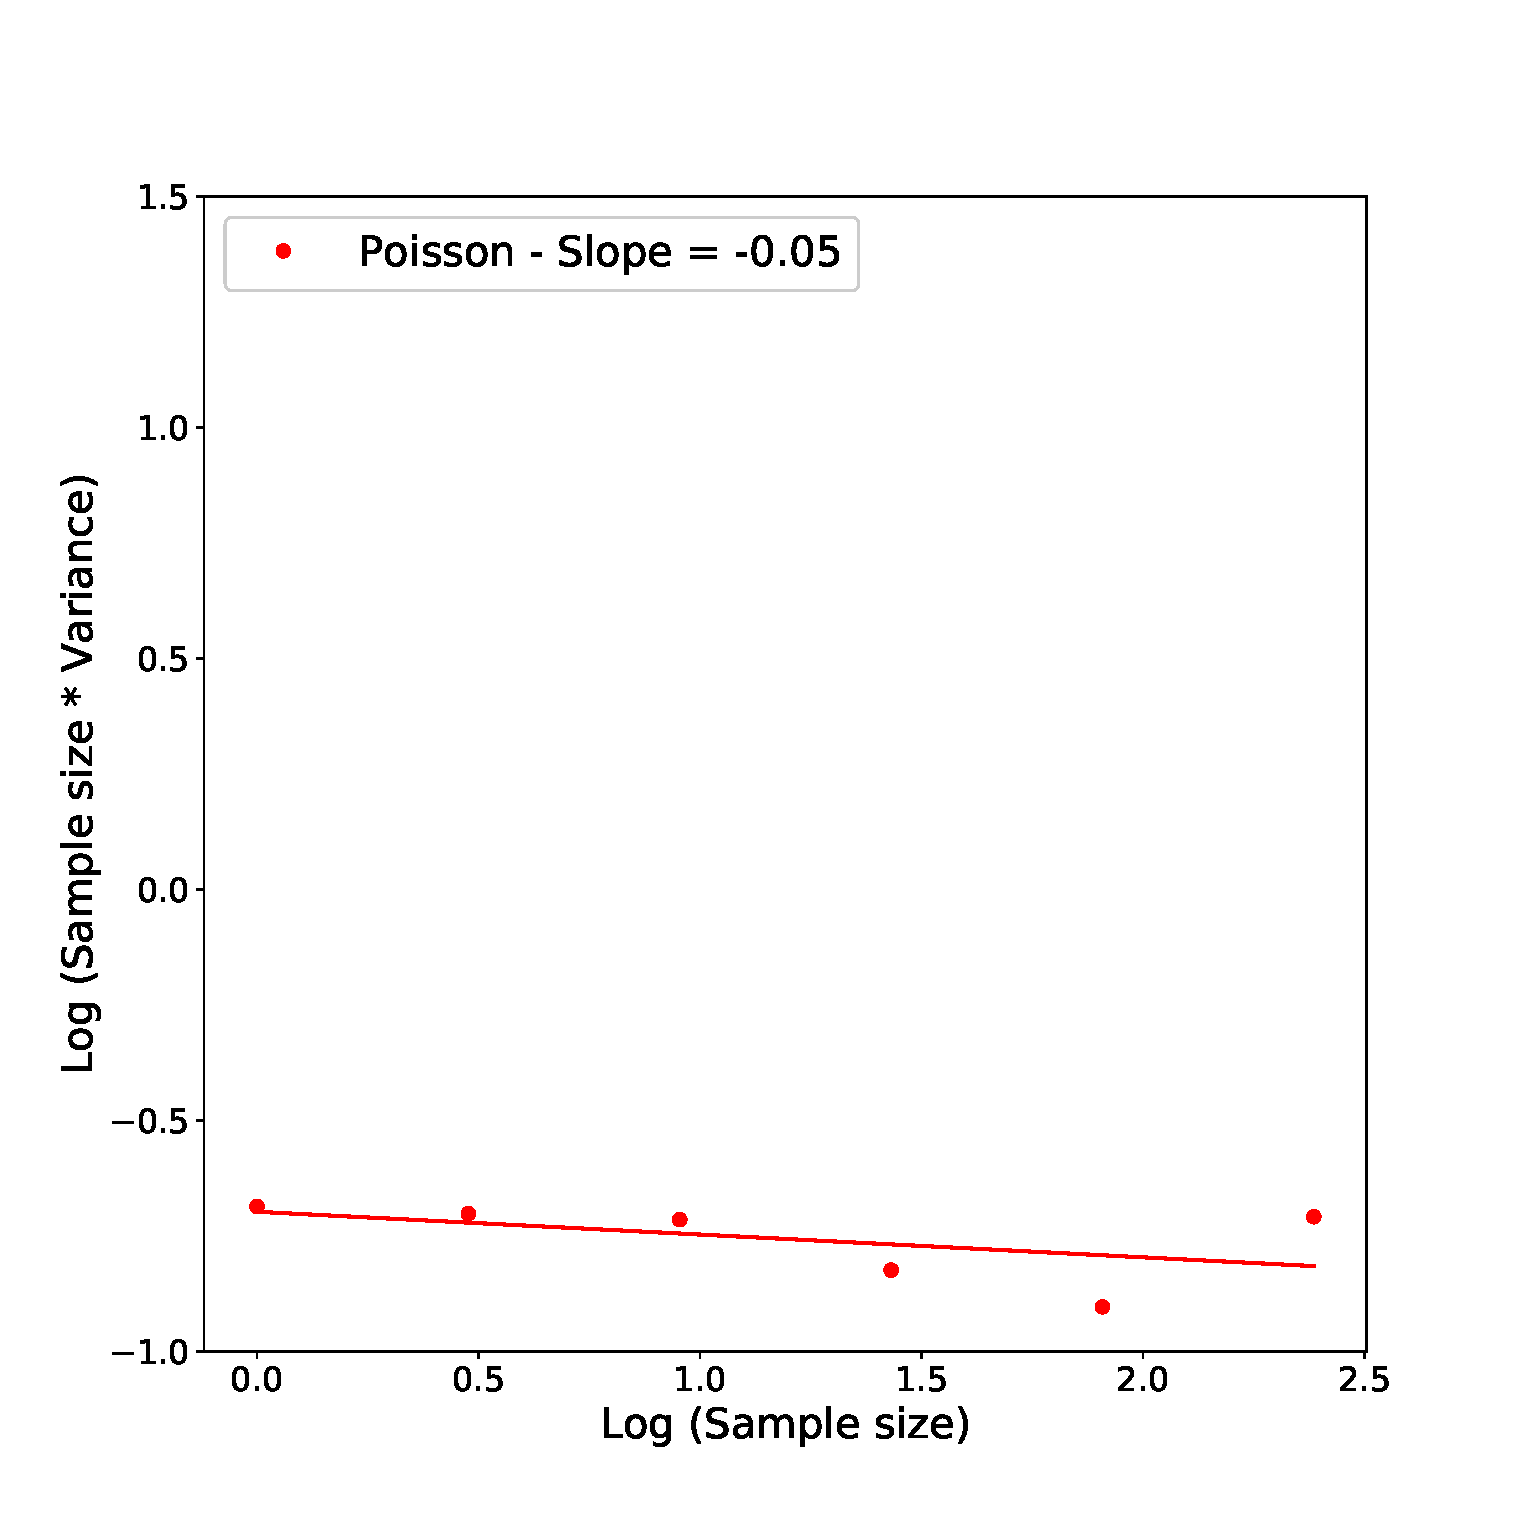
\includegraphics[width=7cm, trim={0cm 1cm 2cm 2cm}, clip]{longrange/comparison_1.eps}
				\end{center}
			\end{column}
		\end{columns}
	\end{frame}

	\begin{frame}
		\frametitle{ETAS model}
		Epidemic-Type Aftershock Sequence (ETAS) model:
		\begin{itemize}
			\item Magnitude frequency distribution law of Gutemberg and Richter
			\item Omori-Utsu law of aftershock decay
			\item Each event, irrespective of whether it is a small or a big event, can trigger its own offspring
		\end{itemize}
		\begin{equation}
		\lambda = \mu + A \sum_{t_i < t} e^{\alpha \left( M_i - M_0 \right)} \left( 1 + \frac{t - t_i}{c} \right) ^{-p}
		\end{equation}
	\end{frame}

	\begin{frame}
		\frametitle{ETAS model}
		\begin{center}
			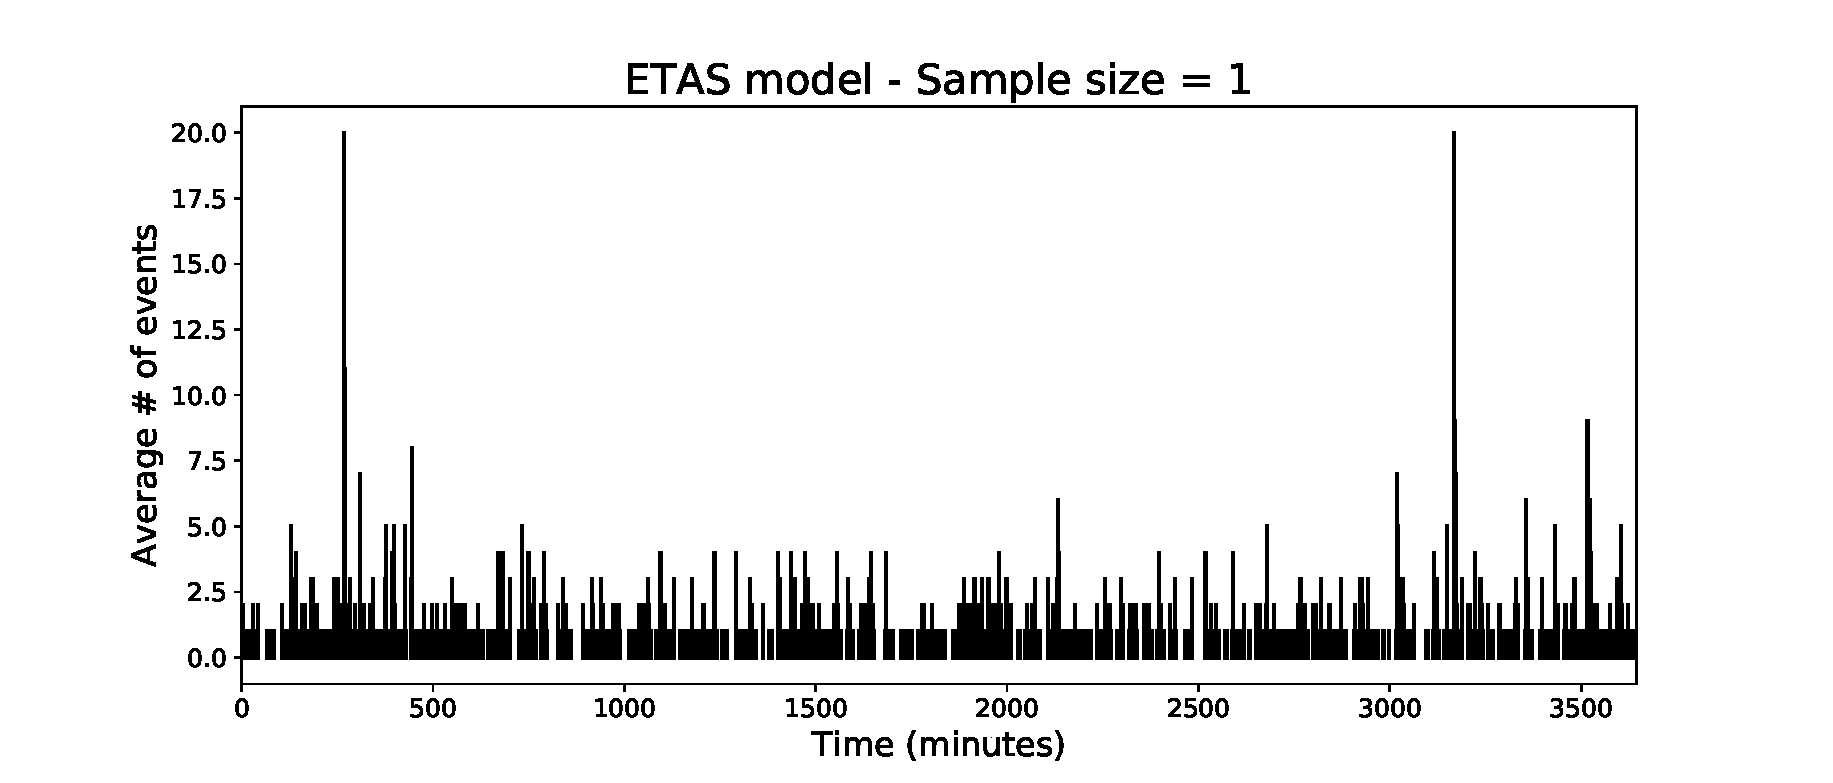
\includegraphics[width=9cm, trim={1cm 0cm 3cm 0cm}, clip]{longrange/ETAS_1.eps}
		\end{center}
		Number of events recorded during one day

		$\rightarrow$ Variance over 3645 values = $0.9636$
	\end{frame}

	\begin{frame}
		\frametitle{ETAS model}
		\begin{center}
			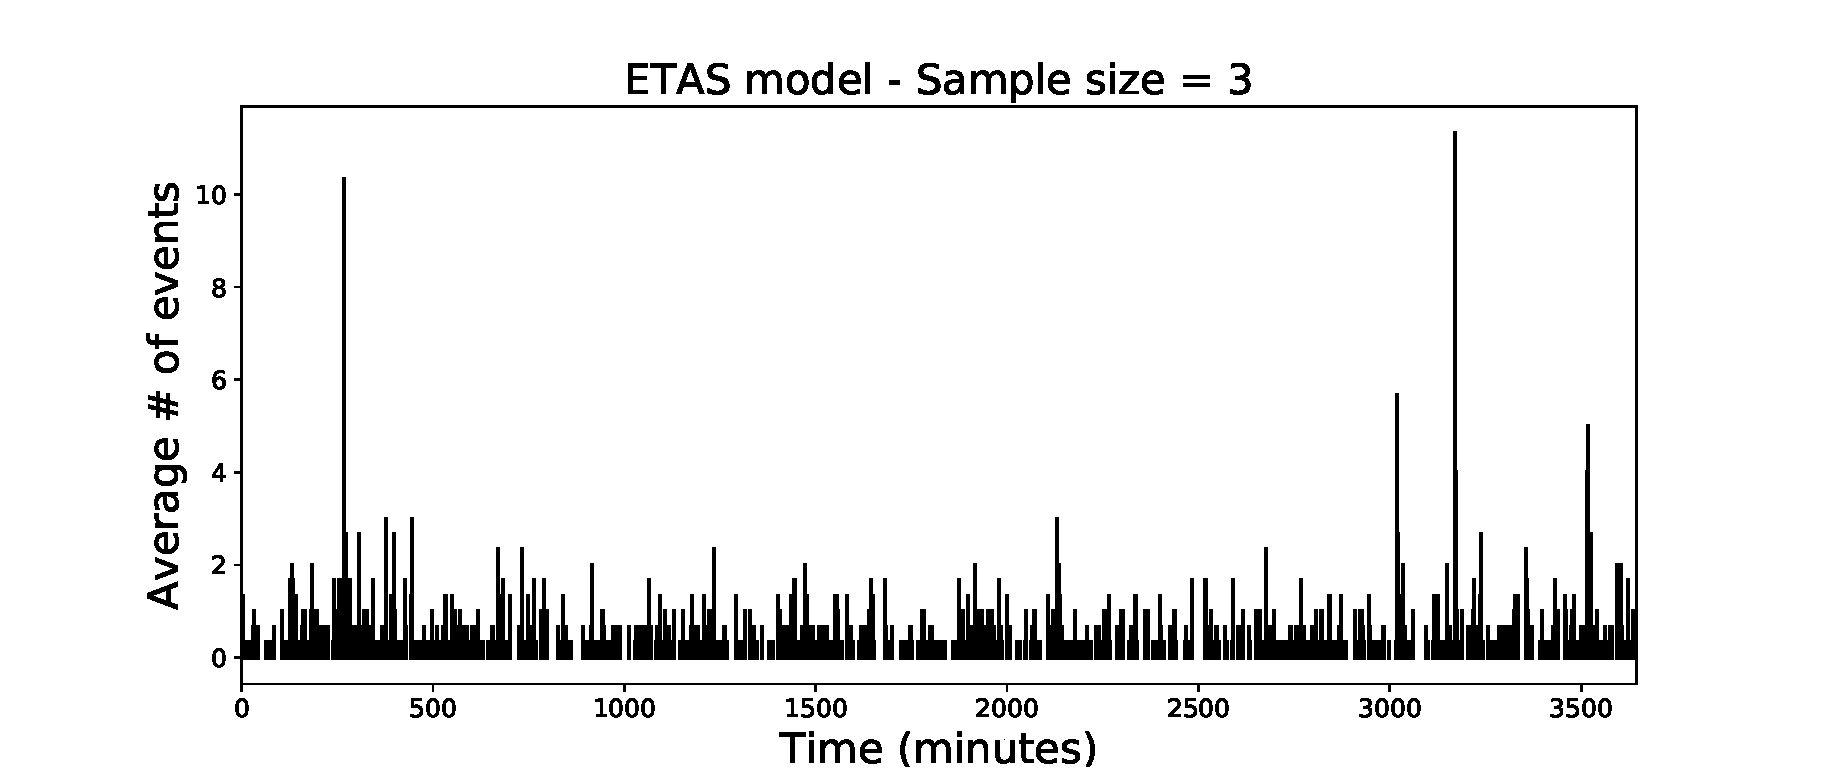
\includegraphics[width=9cm, trim={1cm 0cm 3cm 0cm}, clip]{longrange/ETAS_2.eps}
		\end{center}
		Number of events recorded during 3 days

		$\rightarrow$ Variance over 1215 values = $0.494$
	\end{frame}

	\begin{frame}
		\frametitle{ETAS model}
		\begin{center}
			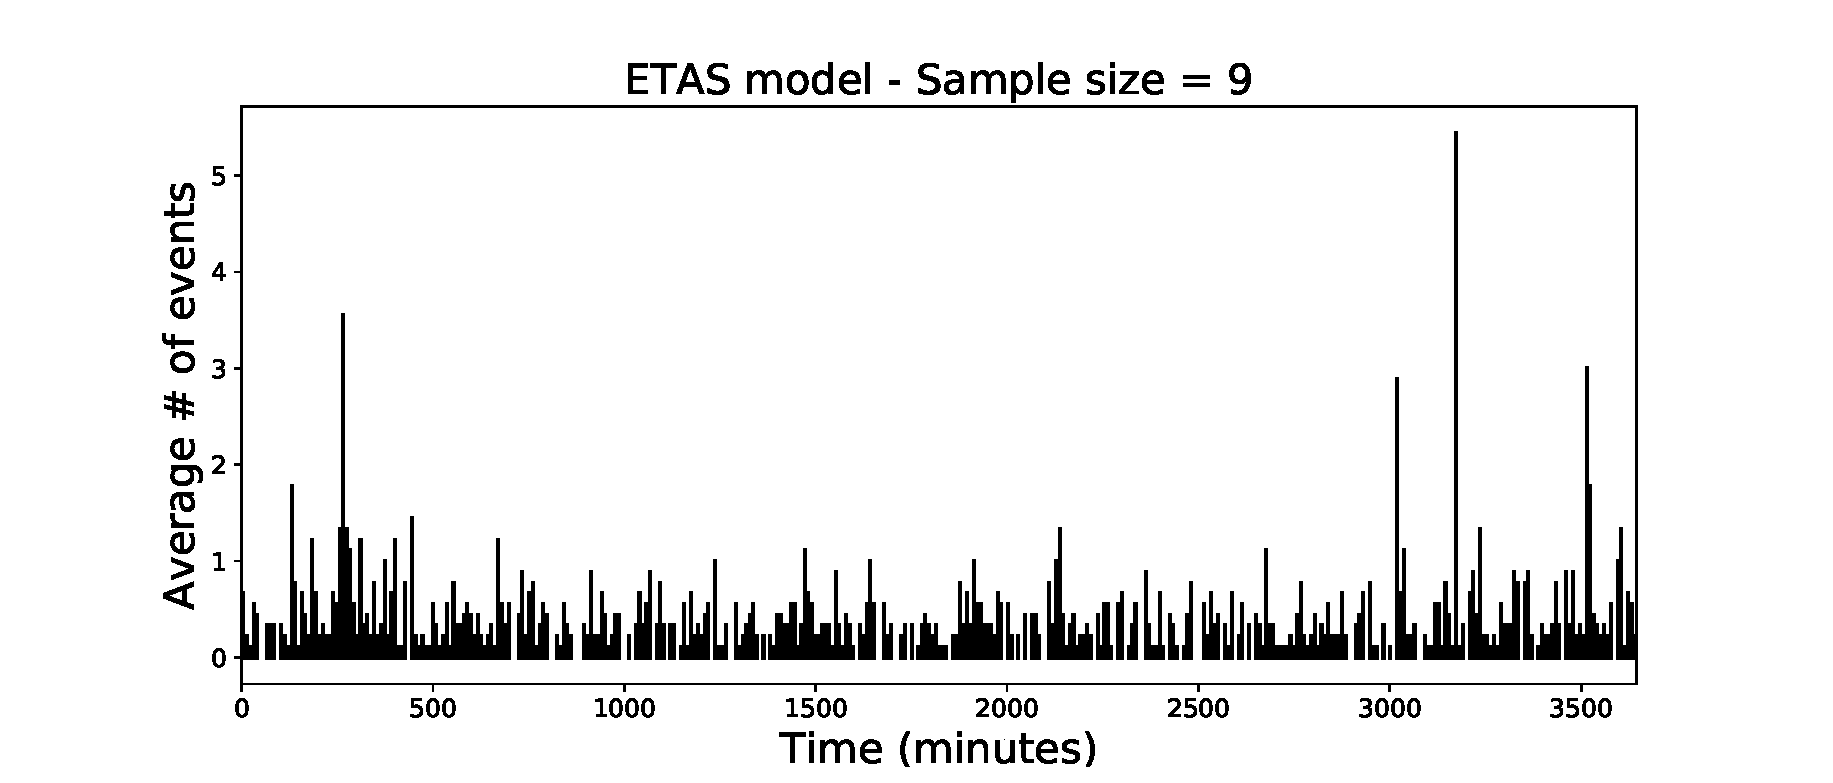
\includegraphics[width=9cm, trim={1cm 0cm 3cm 0cm}, clip]{longrange/ETAS_3.eps}
		\end{center}
		Number of events recorded during 9 days

		$\rightarrow$ Variance over 405 values = $0.220$
	\end{frame}

	\begin{frame}
		\frametitle{ETAS model}
		\begin{center}
			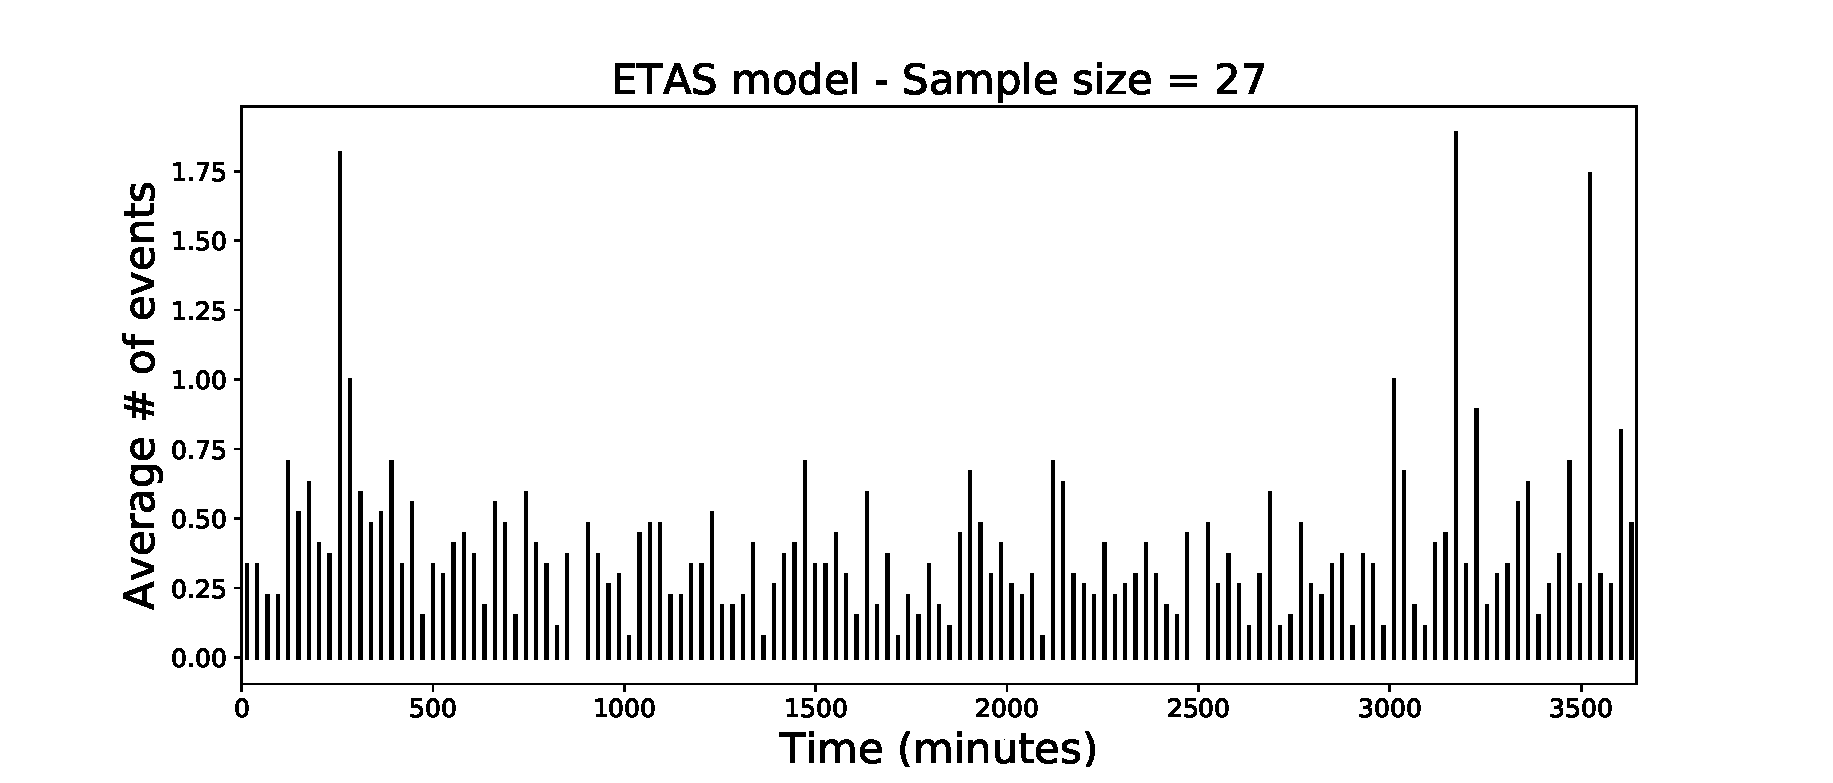
\includegraphics[width=9cm, trim={1cm 0cm 3cm 0cm}, clip]{longrange/ETAS_4.eps}
		\end{center}
		Number of events recorded during 27 days

		$\rightarrow$ Variance over 135 values = $0.0822$
	\end{frame}

	\begin{frame}
		\frametitle{ETAS model}
		\begin{center}
			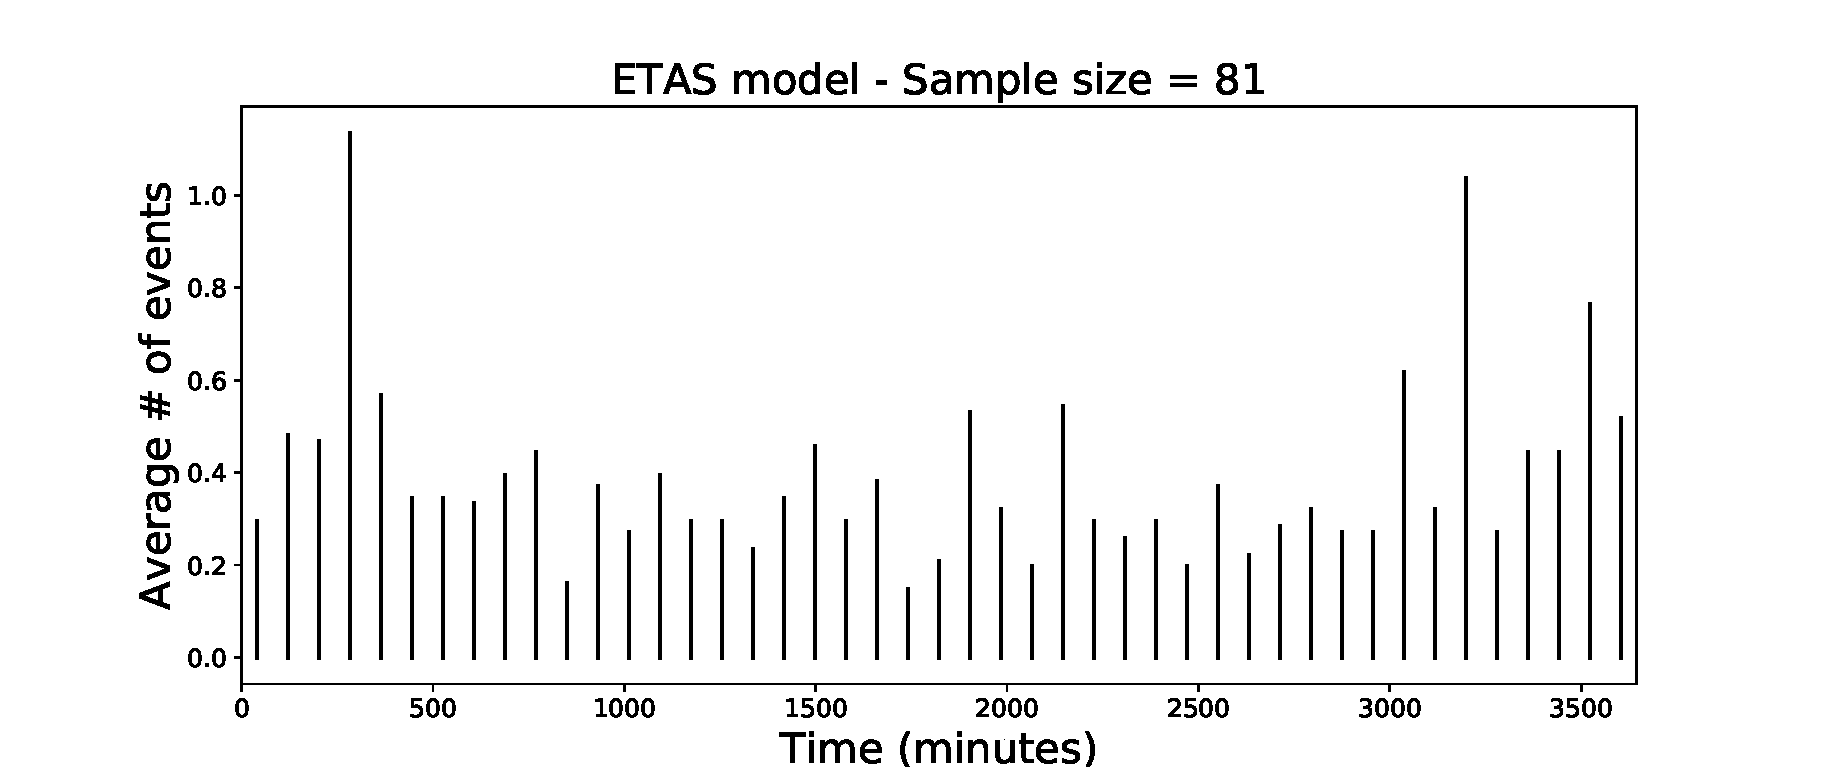
\includegraphics[width=9cm, trim={1cm 0cm 3cm 0cm}, clip]{longrange/ETAS_5.eps}
		\end{center}
		Number of events recorded during 81 days

		$\rightarrow$ Variance over 45 values = $0.0381$
	\end{frame}

	\begin{frame}
		\frametitle{ETAS model}
		\begin{center}
			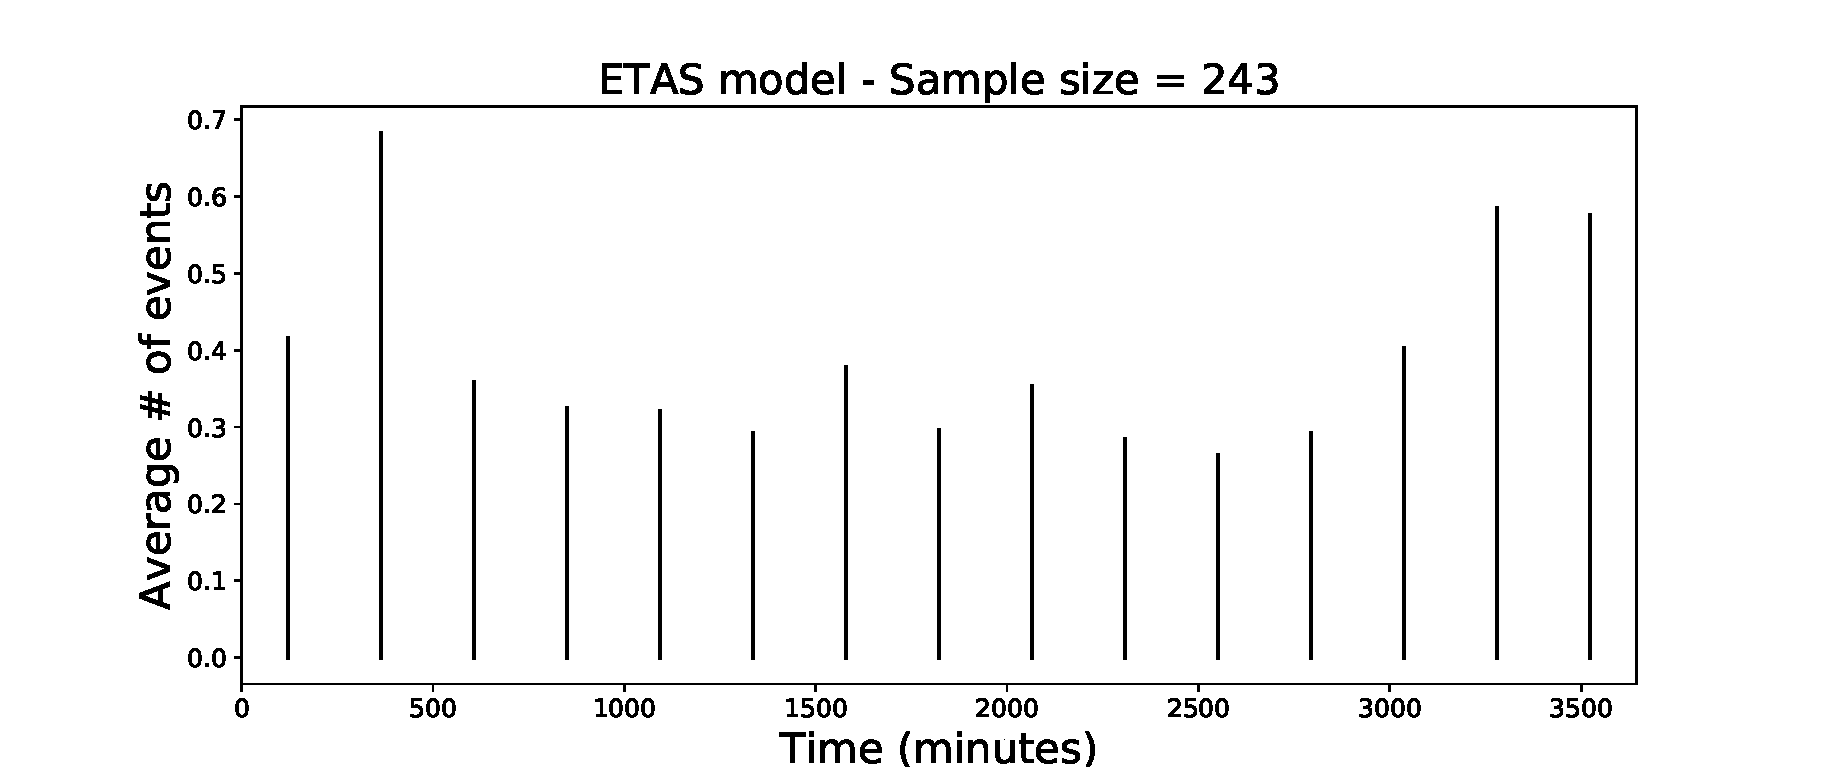
\includegraphics[width=9cm, trim={1cm 0cm 3cm 0cm}, clip]{longrange/ETAS_6.eps}
		\end{center}
		Number of events recorded during 243 days

		$\rightarrow$ Variance over 15 values = $0.0151$
	\end{frame}

	\begin{frame}
		\frametitle{Variance vs Length of time window}
		\begin{columns}[c]
			\begin{column}{4cm}
				$V$ = Variance

				\vspace{1em}

				$m$ = Sample size

				\vspace{1em}

				$V$ behaves as $m^{2 d - 1}$

				\vspace{1em}

				$\rightarrow$ $d =  0.117$
			\end{column}
			\begin{column}{7cm}
				\begin{center}
					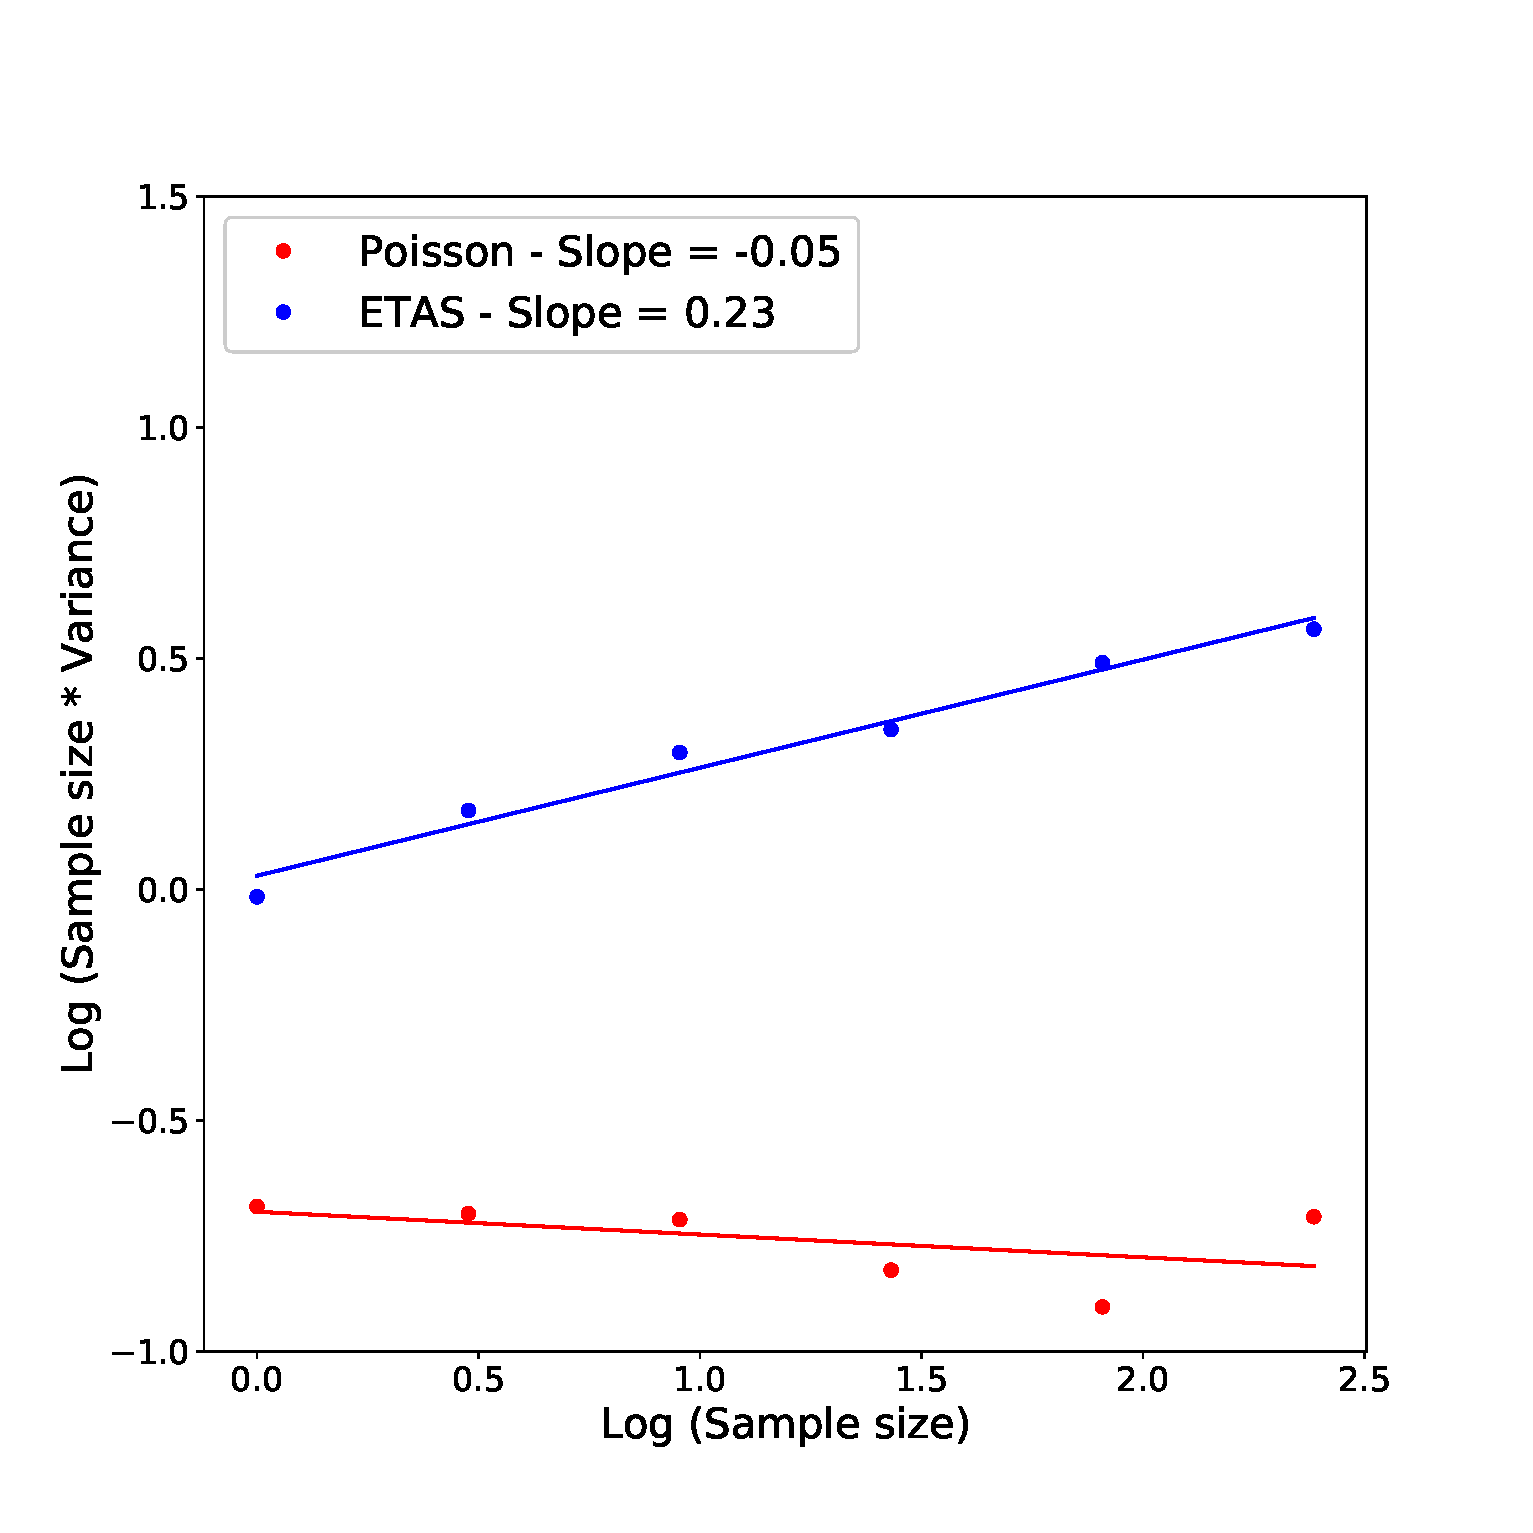
\includegraphics[width=7cm, trim={0cm 1cm 2cm 2cm}, clip]{longrange/comparison_2.eps}
				\end{center}
			\end{column}
		\end{columns}
	\end{frame}

	\begin{frame}
		\frametitle{Northern Cascadia}
		\begin{center}
			\includegraphics[width=5cm, trim={1cm 2cm 2cm 2cm}, clip]{other/cascadia.eps}
		\end{center}
	\end{frame}

	\begin{frame}
		\frametitle{Guerrero, Mexico}
		\begin{center}
			\includegraphics[width=5cm, trim={1cm 2cm 6cm 8cm}, clip]{other/guerrero.eps}
		\end{center}
	\end{frame}

	\begin{frame}
		\frametitle{San Andreas Fault}
		\begin{center}
			\includegraphics[width=5cm, trim={1cm 2cm 1cm 4cm}, clip]{other/sanandreas.eps}
		\end{center}
	\end{frame}

	%----------------------------------------------------------------------------------------------------------------------------------
	% Temporal model of LFE occurrence rate
	%----------------------------------------------------------------------------------------------------------------------------------

	\subsection{Temporal model of LFE occurrence rate}

	\begin{frame}
		\frametitle{Future work}
		\begin{itemize}
			\item Computation of fractional index $d$ for the southern Cascadia catalog
			\item Fit ETAS model on existing LFE families
		\end{itemize}
	\end{frame}
		
	%----------------------------------------------------------------------------------------------------------------------------------
	% Detection of slow slip events in New Zealand
	%----------------------------------------------------------------------------------------------------------------------------------

	\section{Detection of slow slip events in New Zealand}

	\begin{frame}
		\frametitle{Detection of slow slip events in New Zealand}
		\tableofcontents[currentsection,hideothersubsections]
	\end{frame}

	\begin{frame}
		\frametitle{Tremor as proxy for slow slip}
		Episodic Tremor and Slip in Cascadia
		\begin{itemize}
			\item Tremor occurrence rate $\rightarrow$ Moment of slow slip events not detectable in the GPS data (Aguiar, 2009)
			\item Stacking of GPS data when LFEs are detected (Frank, 2016)
		\end{itemize}
		$\rightarrow$ What do we do when tremor is not correlated with slow slip?
	\end{frame}
		
	\begin{frame}
		\frametitle{Northern New Zealand}
		\begin{center}
			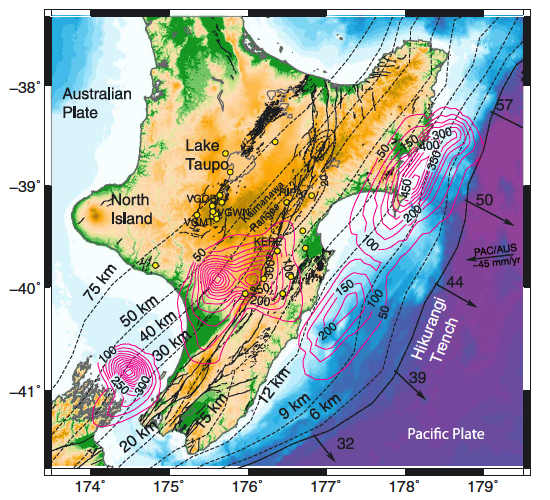
\includegraphics[trim={0cm 0cm 0cm 0cm}, clip, width=7cm]{articles/wallace_eberhart-phillips_2013_1.png}
		\end{center}
	\end{frame}

	\begin{frame}
		\frametitle{Tremor during deep slow slip events}
		\begin{center}
			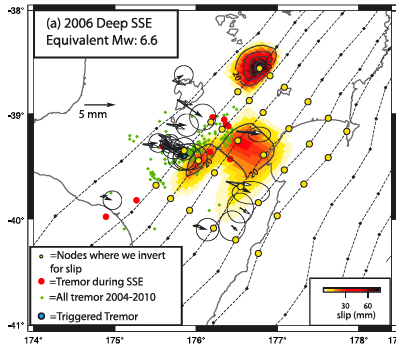
\includegraphics[trim={0cm 0cm 0cm 0cm}, clip, width=7cm]{articles/wallace_eberhart-phillips_2013_3a.png}
		\end{center}
	\end{frame}

	\begin{frame}
		\frametitle{Tremor during deep slow slip events}
		\begin{center}
			\includegraphics[trim={0cm 0cm 0cm 0cm}, clip, width=7cm]{articles/wallace_eberhart-phillips_2013_3b.png}
		\end{center}
	\end{frame}

	\begin{frame}
		\frametitle{Tremor with no detected slow slip event}
		\begin{center}
			\includegraphics[trim={0cm 0cm 0cm 0cm}, clip, width=11cm]{articles/todd_schwartz_2016_6.png}
		\end{center}
	\end{frame}

	\begin{frame}
		\frametitle{Possible questions}
		\begin{itemize}
			\item Detecting smaller, currently undetected slow slip events
			\item Detecting longer term slow slip events
			\item Better measuring of the vertical displacement at the Earth’s surface during slow slip events
		\end{itemize}
	\end{frame}

	\begin{frame}
		\frametitle{Detecting smaller, currently undetected slow slip events}
		\begin{center}
			\includegraphics[trim={0cm 0cm 0cm 0cm}, clip, width=10cm]{articles/wech_creager_2011_3.png}
		\end{center}
	\end{frame}

	\begin{frame}
		\frametitle{Detecting longer term slow slip events}
		\begin{center}
			\includegraphics[trim={0cm 0cm 0cm 0cm}, clip, width=7cm]{articles/wei_al_2012_1.png}
		\end{center}
	\end{frame}

	\begin{frame}
		\frametitle{Better measuring of the vertical displacement at the Earth’s surface during slow slip events}
		\begin{center}
			\includegraphics[trim={0cm 0cm 0cm 0cm}, clip, width=10cm]{slowslip/Prequake_level_changes_shallow_thrust.png}
		\end{center}
	\end{frame}

	\begin{frame}
		\frametitle{Better measuring of the vertical displacement at the Earth’s surface during slow slip events}
		\begin{center}
			\includegraphics[trim={0cm 0cm 0cm 0cm}, clip, width=10cm]{slowslip/Postquake_level_changes_shallow_thrust.png}
		\end{center}
	\end{frame}

	\begin{frame}
		\frametitle{GPS stations in New Zealand}
		\begin{center}
			\includegraphics[trim={1cm 3cm 2cm 6cm}, clip, width=6cm]{Hikurangi/studyarea.eps}
		\end{center}
	\end{frame}

	\begin{frame}
		\frametitle{Denoising of GPS data}
		\begin{center}
			\includegraphics[trim={0cm 0cm 0cm 0cm}, clip, width=11cm]{../slowslip/Figure1.eps}
		\end{center}
	\end{frame}

	\begin{frame}
		\frametitle{Denoising of GPS data}
		\begin{center}
			\includegraphics[trim={0cm 0cm 0cm 0cm}, clip, width=11cm]{../slowslip/Figure2_CKID.eps}
		\end{center}
	\end{frame}

	%----------------------------------------------------------------------------------------------------------------------------------
	% Time line
	%----------------------------------------------------------------------------------------------------------------------------------

	\section{Time line}

	\begin{frame}
		\begin{Huge}
			\begin{center}
				Questions?
			\end{center}
		\end{Huge}
	\end{frame}
			
\end{document}
